\documentclass[a4paper,fontsize=10pt,twoside,DIV15,BCOR12mm,headinclude=true,footinclude=false,pagesize,bibtotoc]{scrbook}

\usepackage[utf8]{inputenc}
\usepackage[T1]{fontenc}

\usepackage{pslatex} % -- times instead of computer modern
\usepackage[scaled=.84]{beramono} % a sane monospace font
\usepackage{microtype}

\usepackage{url}
\usepackage{booktabs}
\usepackage{graphicx}
\usepackage{textcomp}
\usepackage{xspace}
\usepackage[usenames,dvipsnames]{xcolor}
\usepackage{colortbl}
\usepackage{multicol}
\usepackage{rotating}
\usepackage{subfig}
\usepackage{ulem}
\usepackage{enumerate}

% avoid clubs and widows
\clubpenalty=10000
\widowpenalty=10000

% tweak float placement
%% \renewcommand{\textfraction}{.15}
\renewcommand{\topfraction}{.75}
%% \renewcommand{\bottomfraction}{.7}
\renewcommand{\floatpagefraction}{.75}
%% \renewcommand{\dbltopfraction}{.66}
%% \renewcommand{\dblfloatpagefraction}{.66}
\setcounter{topnumber}{4}
%% \setcounter{bottomnumber}{4}
%% \setcounter{totalnumber}{16}
%% \setcounter{dbltopnumber}{4}

\newcommand{\code}[1]{{\texttt{#1}}}
\newcommand{\codefoot}[1]{{\textsf{#1}}}
\def\figref#1{Figure~\ref{fig:#1}}

% ulem package, otherwise emphasized text becomes underlined
\normalem


\newcommand{\todo}[1]{{\emph{TODO: #1}}}
%\renewcommand{\todo}[1]{}

%
% generic command to comment something
%
\newcommand{\comment}[3]{

\textsf{\textbf{#1}} {\color{#3}#2}}

%
% commentators
%
\newcommand{\tommy}[1]{\comment{Tommy}{#1}{Red}}
\newcommand{\wolf}[1]{\comment{Wolfgang}{#1}{OliveGreen}}
\newcommand{\martin}[1]{\comment{Martin}{#1}{Blue}}
\newcommand{\stefan}[1]{\comment{Stefan}{#1}{RoyalPurple}}
\newcommand{\daniel}[1]{\comment{Daniel}{#1}{RoyalBlue}}
\newcommand{\cullmann}[1]{\comment{Christoph}{#1}{Maroon}}
\newcommand{\gebhard}[1]{\comment{Gernot}{#1}{RedOrange}}
\newcommand{\fb}[1]{\comment{Florian}{#1}{Emerald}}
\newcommand{\jack}[1]{\comment{Jack}{#1}{Magenta}}
\newcommand{\sahar}[1]{\comment{Sahar}{#1}{Green}}
\newcommand{\rasmus}[1]{\comment{Rasmus}{#1}{Mahogany}}

%% uncomment to get rid of comments
%\renewcommand{\tommy}[1]{}
%\renewcommand{\wolf}[1]{}
%\renewcommand{\martin}[1]{}
%\renewcommand{\stefan}[1]{}
%\renewcommand{\daniel}[1]{}
%\renewcommand{\cullmann}[1]{}
%\renewcommand{\gebhard}[1]{}
%\renewcommand{\fb}[1]{}
%\renewcommand{\jack}[1]{}
%\renewcommand{\sahar}[1]{}
%\renewcommand{\rasmus}[1]{}

%
% custom colors
%
\definecolor{lightgray}{gray}{0.8}
\definecolor{gray}{gray}{0.5}

\usepackage{listings}

% general style for listings
\lstset{basicstyle=\ttfamily,keywordstyle=\ttfamily}

% listings style for Java
\lstnewenvironment{Java} {\lstset{
  xleftmargin=12pt,
  language=Java
}}{}

\usepackage[endianness=big]{bytefield}

% long immediate in second slot
\newcommand{\lconst}{\texttt{const}_{32}}
% short immediate in ALU instruction
\newcommand{\sconst}{\texttt{Constant}_{12}}
% constant in Rs2 field
\newcommand{\rconst}{\texttt{Constant}_{5}}

% SH: to be used in text mode .. maybe we should change this to math mode?
\newcommand{\XOR}{\textasciicircum\xspace}
\newcommand{\OR}{\textbar\xspace}
\newcommand{\AND}{\&\xspace}
\newcommand{\NOT}{\texttildelow}
\newcommand{\shl}{\textless$\!$\textless\xspace}
\newcommand{\shr}{\textgreater$\!$\textgreater$\!$\textgreater\xspace}
\newcommand{\ashr}{\textgreater$\!$\textgreater\xspace}

\newcommand{\bitsunused}{\rule{\width}{\height}}
\newcommand{\bitssubclass}{\color{lightgray}\rule{\width}{\height}}

%
% allow click-able links
%
\usepackage[open]{bookmark}
\usepackage[all]{hypcap}

%
% hyperref setup (depends on bookmark/hyperref}
%
\hypersetup{
    pdftitle = {Patmos Reference Handbook},
    pdfsubject = {Technical Report},
    colorlinks = {true},
    citecolor = {black},
    filecolor = {black},
    linkcolor = {black},
    urlcolor = {black},
    final
}

%
% document contents
%
\begin{document}

\title{Patmos Reference Handbook}

\author{Martin Schoeberl, Florian Brandner, Stefan Hepp,\\Wolfgang Puffitsch, Daniel Prokesch}

\lowertitleback{\todo{Copyright and license terms come here.}}

\frontmatter

\maketitle

\chapter{Preface}

This TR shall evolve to the documentation of Patmos. In the mean time
it is intended to collect design notes and discussions.  Especially
ISA design notes now.

\section*{Acknowledgment}

We would like to thank Tommy Thorn for the always intense and enjoyable
discussions of the Patmos ISA and processor design in general.
Jack Whitham offered his experience with RISC
ISA design and trade-offs. 
Gernot Gebhard and Christoph Cullmann gave valuable feedback on the ISA
relative to WCET analysis.
Sahar Abbaspourseyedi is working on the stack
cache and verifies the ideas and concepts presented here. We thank
Rasmus Bo Sørensen for fixing some documentation errors.

This work was partially funded under the
European Union's 7th Framework Programme
under grant agreement no. 288008:
Time-predictable Multi-Core Architecture for Embedded
Systems (T-CREST).

\tableofcontents

\begingroup
\let\cleardoublepage\clearpage
\listoffigures
\listoftables
%\lstlistoflistings
\endgroup

\mainmatter

\chapter{Introduction}

Real-time systems need a time-predictable execution platform so that the worst-case execution time (WCET) can be statically estimated. It has been argued that we have to rethink computer architecture for real-time systems instead of trying to catch up with new processors in the WCET analysis tools~\cite{tpca:jes, pret:dac2007}.

We present the time-predictable processor Patmos as one approach to attack the complexity issue of WCET analysis. Patmos is a static scheduled, dual-issue RISC processor that is optimized for real-time systems.



%\chapter{Related Work}
%\label{sec:related}


\fb{Martin wishes that Patmos will not require more than 3000 LC ;-)}
\martin{And fmax shall not be below 80\% of NIOS or MicroBlaze.
And performance (also average case ;-) shall be better, compared to NIOS/MB.
And we could compare against Tommy's YARI.}

\martin{TODO: The instruction description with the individual pipeline stages shall be
rewritten to reflect the actual simulator and hardware implementation of Patmos.
E.g. predicate registers are *not* read in the decode stage, but directly in EX.
Reading in decode would mean a one cycle generate use delay.}

\section{TODO}

This report shall converge towards a real manual. At the moment it serves
discussion well, but we shall keep this in mind. Here a starting list of TODOs:

\begin{itemize}
\item Send an email to all and ask about cleanup of some discussion points
\item Convert some discussion text into readable sections and argue why we
did what we did
\item Get a nice introduction and a good architecture section written
\end{itemize}

\section{Pending Changes}

This is a live and temporary section that lists pending changes of the ISA.
This changes shall live in a remote branch (to be specified) and have a
date when to be merged into the master branch.

Currently we have following proposals for a change:

\begin{itemize}
\item bcopy instruction
\item btest and bcopy with an immediate
\item Automatic save of method base in a special register for a call
\item Branch into subfunction
\item Revised branch addressing modes
\item Non-delayed branches
\item Issue memory operations from any pipeline
\item Interrupts
\end{itemize}

Remote branch: not specified

Merge date: 15 August 2013 (?)

\subsection{\texttt{bcopy}/\texttt{btest}}

\wolf{Please describe the requested change.}

\subsection{Special Registers for Return Information}

In order to support exceptions (see Section~\ref{sec:exc}), it is
necessary that the base address of the current function is available
\emph{at any time}. Otherwise, it could not be guaranteed that an
interrupt handler is able to return to the correct
function. Consequently, the \texttt{call} and \texttt{brcf} functions
must store the base address in some hardware register. This makes the
return-base information in register \texttt{r30} redundant and it
could be replaced by an appropriate special return base register
\texttt{sb} with minimal effort. One can then go even further and move
the functionality of register \texttt{r31} to a special register
\texttt{so} to free up another general-purpose register.

\stefan{This is actually how we had it in the first ISA version, but Martin wanted to get rid of 
the special registers.. ;) }

\stefan{Note that we could still make this part of the ABI: we can simply require that \texttt{r30} is 
never used for something else and must always contain the valid base address (this is the case at the moment 
except for (sub)functions that do not have calls inside, can be changed easily). The bigger issue I see is
that there are problems when the interrupt appears between the \texttt{call} and the \texttt{ldi} that sets 
\texttt{r30} (they cannot be bundled), and a scheduler might further move the load around.}

\wolf{The latter issue is exactly the problem. The hardware needs to
  keep track of the base whenever a \texttt{call}, \texttt{brcf} or
  \texttt{ret} is executed to be able to return from interrupts at any
  time. The question is if we move the current base to a visible
  register upon calls to serve as return base. It is not necessary,
  but why keep track of the base both in hardware and in software?
  Note that the hardware does not need to expose the current base,
  only the return base would be made visible.}
  
\martin{Agree on that.}

\stefan{And I was so happy not to have both \texttt{S0} and \texttt{SO} in the compiler anymore ;) I would suggest to call them 
\texttt{srb} and \texttt{sro} instead (for return base and return offset, which they actually are).}

\wolf{Agree for \texttt{srb} and \texttt{sro}.}

\subsubsection{Costs and Benefits}

For functions that call other functions, the change saves one
instruction to set the base address, and adds two instructions to both
the prologue and the epilogue. On the other hand, the change frees up
two general-purpose registers, which can avoid spilling and lead to
more efficient code.

\stefan{It also saves some logic in the function splitter to calculate
the code size increase due to the requirement to set the base address in all
new sub-functions that contain a call.}

\subsection{Branch into Subfunction Instruction}

\stefan{In order to eliminate the current restriction of having only single-entry subfunctions, 
I would suggest to make \texttt{brcf} indirect accept both an (absolute) base address, as well 
as an offset. Using \texttt{r0} for the offset makes \texttt{brcf} behave similar to now. 

At the moment we could also use \texttt{ret} for the same purpose, but this has two disadvantages:
\texttt{call} and \texttt{ret} would no longer appear in pairs, making call graph reconstruction more complicated 
(needs compiler support to tell the WCET analysis which \texttt{ret} is actually used as return), and it
does not work nicely if we change \texttt{ret} to use special registers.}

\wolf{If I understand correctly, indirect \texttt{brcf} would then do
  exactly the same thing as \texttt{ret} does currently, except that
  it gets a different opcode. I don't see a problem with that from the
  hardware perspective.}

\stefan{Correct. With moving return infos to special registers, \texttt{ret} would become different from \texttt{brcf} though as 
\texttt{ret} would use \texttt{srb} and \texttt{sro}, I presume, while \texttt{brcf} always uses two GPRs.}

\subsubsection{Costs and Benefits}

Much of the complexity and restrictions of the function splitter are eliminated (jump tables
still have to be handled carefully, though we in theory we could even support having jump table entries 
anywhere in any region), without resorting to misuse \texttt{ret}. It works regardless of whether return information
is stored in special registers or GPRs.

To make use of this feature, the function splitter needs a major rewrite though. 
Note that as long only \texttt{r0} is used for the offset, no changes to the compiler or the WCET analysis are required.

\stefan{It also moves \texttt{brcf} from \texttt{CFLi} to \texttt{CFLr}, which makes the naming of the formats less intuitive 
(although having \texttt{CFLi} for register operands is not good anyway, as we usually use \texttt{i} for immediate).}

\wolf{I guess the naming of the formats is not our biggest concern ;-)}

\subsection{Revised Branch Addressing Modes}

\wolf{I propose to change the branch addressing modes as shown in
  Table~\ref{tab:braddr}.}

\begin{table}
  \centering
  \begin{tabular}{lllll}
    \toprule
    Instruction & Immediate             & Indirect                   & Cache fill & Link \\
    \midrule
    call        & absolute              & absolute                   & yes        & yes \\
    br          & PC relative           & \color{red}{base relative} & no         & no \\
    brcf        & \color{red}{absolute} & absolute                   & yes        & no \\
    \bottomrule
  \end{tabular}
  \caption{Revised branch addressing modes}
  \label{tab:braddr}
\end{table}

\subsubsection{Rationale}

With a method cache, there are two distinct views of the program
counter: the program counter to address the cache memory
(PC$_{cache}$), and the address of the respective instruction in
memory (PC$_{mem}$). When loading instructions from memory
(\code{call}, \code{brcf}), PC$_{mem}$ is relevant, because it
specifies from where data should be loaded. However, when execution
remains within a function (\code{br}), only PC$_{cache}$ is taken into
account.

Listing~\ref{lst:call} shows the pseudo-code for a call (using special
registers \texttt{sb} and \texttt{so} for the return
information). First, it stores the return information, and remembers
the new base address. Then, it retrieves the offset into the cache for
the function to be called and if necessary copies the instructions
into the cache. Finally, it updates the internal program counter and
continues execution from there.

\martin{I do not understand those listing fully. E.g. what those variables
are: intern registers, special registers,... However, I very much appreciate
this pseudo code. That should then go into the `normal' ISA description as
well.}

\begin{lstlisting}[language=C,mathescape=true,float=t,caption={Call\label{lst:call}}]
call(addr) {
  // Store return information
  sb = base;
  so = PC$_{cache}$;  
  // Remember base address
  base = addr;
  // Cache look-up and load
  coff = offset(addr);
  if (!hit(base)) memcpy(cache[coff], mem[base], mem[base-4]);
  // Update PC
  PC$_{cache}$ = coff;
}
\end{lstlisting}

Listing~\ref{lst:return} shows the pseudo-code for a return. It first
retrieves the return base and does the appropriate cache handling. It
then adds the cache offset and the return offset and assigns the sum
to the internal program counter, from which execution continues.

\begin{lstlisting}[language=C,mathescape=true,float=t,caption={Return\label{lst:return}}]
ret() {
  // Retrieve return base
  base = sb;
  // Cache look-up and load
  coff = offset(sb);
  if (!hit(base)) memcpy(cache[coff], mem[base], mem[base-4]);
  // Update PC
  PC$_{cache}$ = coff+so;
}
\end{lstlisting}

The pseudo-code for a PC-relative \texttt{brcf} is shown in
Listing~\ref{lst:brcfrel}. It is similar to the call, but does not
store any return information. However, before being able to do any
cache handling, it has to compute the actual address, given by
\code{base-coff+PC$_{cache}$+off}. Even when precomputing
\code{base-coff}, this includes two additions that increase the
hardware overhead.

\begin{lstlisting}[language=C,mathescape=true,float=t,caption={PC-relative \texttt{brcf}\label{lst:brcfrel}}]
brcf(off) {
  // Compute actual address
  addr = base-coff+PC$_{cache}$+off;
  // Remember base address
  base = addr;
  // Cache look-up and load
  coff = offset(addr);
  if (!hit(base)) memcpy(cache[coff], mem[base], mem[base-4]);
  // Update PC
  PC$_{cache}$ = coff;
}
\end{lstlisting}

Listing~\ref{lst:brcfabs} shows the pseudo-code for \texttt{brcf} with
absolute addressing. It avoids the address computation of the
PC-relative \texttt{brcf} and thus reduces the hardware overhead.

\begin{lstlisting}[language=C,mathescape=true,float=t,caption={Absolute \texttt{brcf}\label{lst:brcfabs}}]
brcf(addr) {
  // Cache look-up and load
  base = addr;
  coff = offset(addr);
  if (!hit(base)) memcpy(cache[coff], mem[base], mem[base-4]);
  // Update PC
  PC$_{cache}$ = coff;
}
\end{lstlisting}

The argument for base-relative indirect branches is more subtle. In
any case, the instruction requires an addition or subtraction
(absolute: \code{PC$_{cache}$ = addr-base+coff}, base-relative:
\code{PC$_{cache}$ = addr+coff}, PC-relative: \code{PC$_{cache}$ =
  PC$_{cache}$+addr}). The address information for indirect branches
only becomes available in the execute stage, because the value might
require forwarding. Keeping this addition as cheap as possible avoids
putting stress on the timing of the path from the execute stage to the
fetch stage. Of the three variants, the addition \code{addr+coff} is
``cheapest'', because the lowest bits of \code{coff} are cleared due
to the guaranteed alignment of functions to cache blocks in the method
cache.

\stefan{I am kind of OK-ish with changing brcf immediate to absolute, if it is absolutely necessary (assuming that we do not need to address
code above 16MB, otherwise we cannot use an immediate absolute brcf!), though I do not really want to touch that code in the tool chain and 
loose compatibility with a3 again (if someone else takes care of all that, feel free to go ahead though ;) ).}

\wolf{Regarding the size limitation: If the code grows above 16MB, we
  have to issue indirect calls as well. I don't see a real problem
  with issuing indirect \texttt{brcfs} in that case (there is a
  reserved scratch register somewhere, right?). The change in the tool
  chain is -- unless I am missing something big -- roughly 5 lines of
  code to give the instruction a different relocation type. Losing
  compatibility with a3 is an issue, but my guess would be that the
  changes on their side are similarly simple.}

\stefan{The advantage of PC indirect brcf is that even if we have code above 16MB (the code does not need to be that large,
it might just be a result of the address mapping), we might still simply assume not to have any single function larger than 
8MB. In this case, we only need to take care of \texttt{call}, not of \texttt{brcf}. 

From a compiler point of view, \texttt{br} and \texttt{brcf} really are the same. Any difference there just introduces some more complexity
to the function splitter (as it needs to track code sizes and generated code carefully). Since we already have the absolute immediate
relocation type though, the change is indeed not a big one (assuming no code above 16MB).}

\stefan{However, I strongly oppose changing any of the indirect branches to anything else than absolute, it makes quite a mess 
in the compiler backend and the linker (and probably the analysis). The problem here are jump tables, which are 
kind of outside of the function and have no clear reference to the function, making the calculation of any base offset in the linker quite
complicated (you need to introduce a new relocation type, change the relocation type of the jump table symbols depending on the way they are
used, and calculate the symbol value in the linker by finding the (already relocated!) surrounding sub-function symbol).}

\wolf{The base-relative address difference does not need ``real''
  relocation, because basic blocks always have the same distance to
  the function entry. Everything you need in the linker is already
  there for the \texttt{.fsize} and \texttt{.size} directives. I am
  not sure how much trouble it is to have LLVM emit the difference of
  two symbols for jump tables, but it is definitely possible. That
  being said, I could live with leaving indirect branches as they are,
  I just don't think that it's the most efficient solution.}
  
\martin{I'm with Wolfgang on the timing issue of having two
additions (one operand coming from the register forward path)
going into the dual issue fetch stage is an issue.

If we really want to avoid changing the br indirect right now,
a work around would be to make it a two cycle stalling instruction.}

\stefan{How about pre-calculating \code{coff-base} at \texttt{call}/\texttt{brcf}/\texttt{ret}? It costs one 32bit register (or
30bit assuming alignment) and an additional op at those instructions, but saves the second subtract at \texttt{br} (note that we cannot 
use the second ALU for a \texttt{call} and most likely never will use it for \texttt{brcf} as long as it has one cycle more than \texttt{br}
since it is only introduced after the scheduler and replaces a \texttt{br}).} 

\wolf{Precalculating is what we should anyway if we keep things as
  they are. Still, all bits of the addend \code{coff-base} are
  significant, while \texttt{coff} has its lowest bits
  cleared. Imagine a method cache with 32KB and 128 functions. With
  word addressing, PC$_{cache}$ and \texttt{coff} would be 13
  bits. The lowest 6 bits of \texttt{coff} would be guaranteed zero
  due to alignment. Consequently, the complexity of the addition is
  almost cut in half (13 significant bits vs 7 significant bits).

  What do you mean exactly with ``we cannot use the second ALU for a
  \texttt{call}''?}

\stefan{Due to the fixed size of the call delay slot, we are never allowed to issue anything in parallel with a call anyway, so from my
naive point of view we should have the second ALU available to do the precalculation ;) }


\stefan{Another reason apart from the linker issue is that debugging becomes harder, as
the binary no longer contains absolute addresses at jump tables, but one has to know the base of the current sub-function (which is usually
not obvious from just looking at the disassembly) and add the values to get the actual target addresses, and you cannot grep for the
addresses in the disassembly easily. Debugging some jump table/method cache related bugs in the compiler backend is already quite painful as it is..}

\subsection{Non-delayed Branches}

Delayed branches are a good means to hide the costs of branching.
However, the compiler is not always able to fill the delay slots. In
these cases, even a primitive strategy such as predict-not-taken
provides better performance. Predict-not-taken has very little
hardware overhead and can be modeled easily in an exact manner for
WCET analysis. By introducing an \emph{additional} instruction for
non-delayed immediate branches, Patmos can gain from the advantages of
both delayed and non-delayed branches.

Furthermore, having a non-delayed branch instructions enables research
towards time-predictable branch-prediction schemes. Depending on our
future findings, predict-not-taken could be replaced by
predict-backward-taken or time-predictable forms of dynamic branch
prediction to further improve both performance and WCET bounds.

\stefan{But this would introduce the need to take care of exceptions in hardware that might
arise due to a mis-predicted branch, e.g., due to a load at the beginning of
the fallthrough target, right?}

\wolf{Nope. A mispredicted branch is detected in the execute stage and
  flushes the instructions that are currently in the fetch and the
  decode stage. The flushed instructions never make it to the execute
  stage, which would be the earliest place where any effect could
  become visible.}
  
\martin{Very much in favor to this addition.}

\stefan{Also agree, and I would like to have this for both \texttt{br} and \texttt{brcf} (function splitter ...). This could 
at least save quite some code space and reduce the overestimations in the function splitter quite a lot.

We should really get a proper scheduler though to support this properly, the current delay slot filler is getting more and more 
scary..}

\wolf{Non-delayed \texttt{brcf} should be okay, the stages that need
  to be flushed are the same as for interrupts.}

\subsection{Issue Memory Operations in any Pipeline}

Allow stack cache accesses, maybe even any memory access in the second pipeline, as long as there is no memory access to the same 
memory executed in the first pipeline.

\begin{lstlisting}
  { (p1) sws [1] = $r1  ; (!p1) sws [3] = $r2 }   # allowed, only one predicate is true
  {      swc [r1] = $r4 ;       sws [2] = $r4 }   # allowed, different memories
  {      br  -4         ;       swl [$r1] = $r2 } # could also be allowed
  {      ret            ;       swc [$r1] = $r2 } # could also be allowed
  {      sws [4] = $r1  ;       sws [5] = $r2  }  # not allowed
\end{lstlisting}

\subsubsection{Costs and Benefits}

In contrast to the original plan, we do not need to have a double-clocked stack cache, but are still able to spill in the second
pipeline while the first pipeline is either accessing main memory or doing control flow, and we can schedule if-converted code and
single-path code more in parallel.

While this does not improve the situation for blocks with large sequences of spills,
e.g. at prologues and epilogues, it might improve the situation for code with lots of control-flow or if-converted code, even in
situations where a double-clocked stack cache access alone does not help.

\stefan{I frankly do not know how much this will actually gain since usually the code contains either
main memory access or stack access, not so much a mixture of both, and we need a proper scheduler and play around with the if-converter first to
see how much ILP we can get out of the code. 

Martin promised to take a real serious look at it when we can get some figures showing a gain from the compiler.. ;) }

\wolf{I oppose this change. It's quite a bit of hardware, and
  performance gains are most likely negligible. There is not much else
  to do in the prologue/epilogue, and stack accesses are relatively
  rare elsewhere. If you can show a realistic example where
  performance gains are significant, I might change my mind.

  Note that we cannot mix XXc and XXm, because both might go to main
  memory in case of a cache miss. Stack control and
  \texttt{call}/\texttt{brcf} conflict with both XXc and XXm.}

\subsection{Interrupts and Exceptions}

See Section~\ref{sec:exc} for the proposed implementation and changes
to the ISA to support interrupts and exceptions in Patmos.

\chapter{The Architecture of Patmos}
\label{sec:arch}

\section{Pipeline}

Figure~\ref{fig:pipeline} shows an overview of Patmos' pipeline. The pipeline
consist of 5 stages: (1) instruction fetch (\texttt{FE}), (2) decode and
register read (\texttt{DEC}), (3) execute (\texttt{EX}), (4) memory access (\texttt{MEM}), and (5) register write  back (\texttt{WB}).

Some instructions define additional pipeline stages. Multiplication instructions
are executed, starting from the \texttt{EX} stage, in a parallel pipeline with
fixed-length (see the instruction definition). The respective stages are
referred to by \texttt{EX$_1$}, \dots, \texttt{EX$_n$}.

\martin{\todo{A more detailed description of the pipeline stages, as the individual
4 stage description is gone.} Here a start:}

\subsection{Fetch}

Fetch one or two words of instruction from the ROM or method cache.
Calculate next PC depending on the length of the instruction bundle.

\subsection{Decode}

Decode the instruction and generate control signals for the following stages.
Read register operands. Sign or zero extend immediate operands.

\subsection{Execute}

Read predicate registers. Conditional execute (ALU) instructions.
Write predicate register. Calculate effective address for memory operations.

\subsection{Memory}

Read or write memory. This is the only pipeline stage that might
stall the pipeline.

\subsection{Write Back}

Write result into destination register.

\stefan{Note that in the \texttt{pasim} simulator the Memory and Write Back stages are merged into a single MW stage at the time of writing,
and the stages are simulated from back to front.
While this has no effect on the timing and hazards of the instructions, there is only a single bypass from MW to EX (per pipeline). Apart
from that, all implementations of all instructions in the simulator should adhere to the above description of the stages.}

\begin{figure}
    \centering
    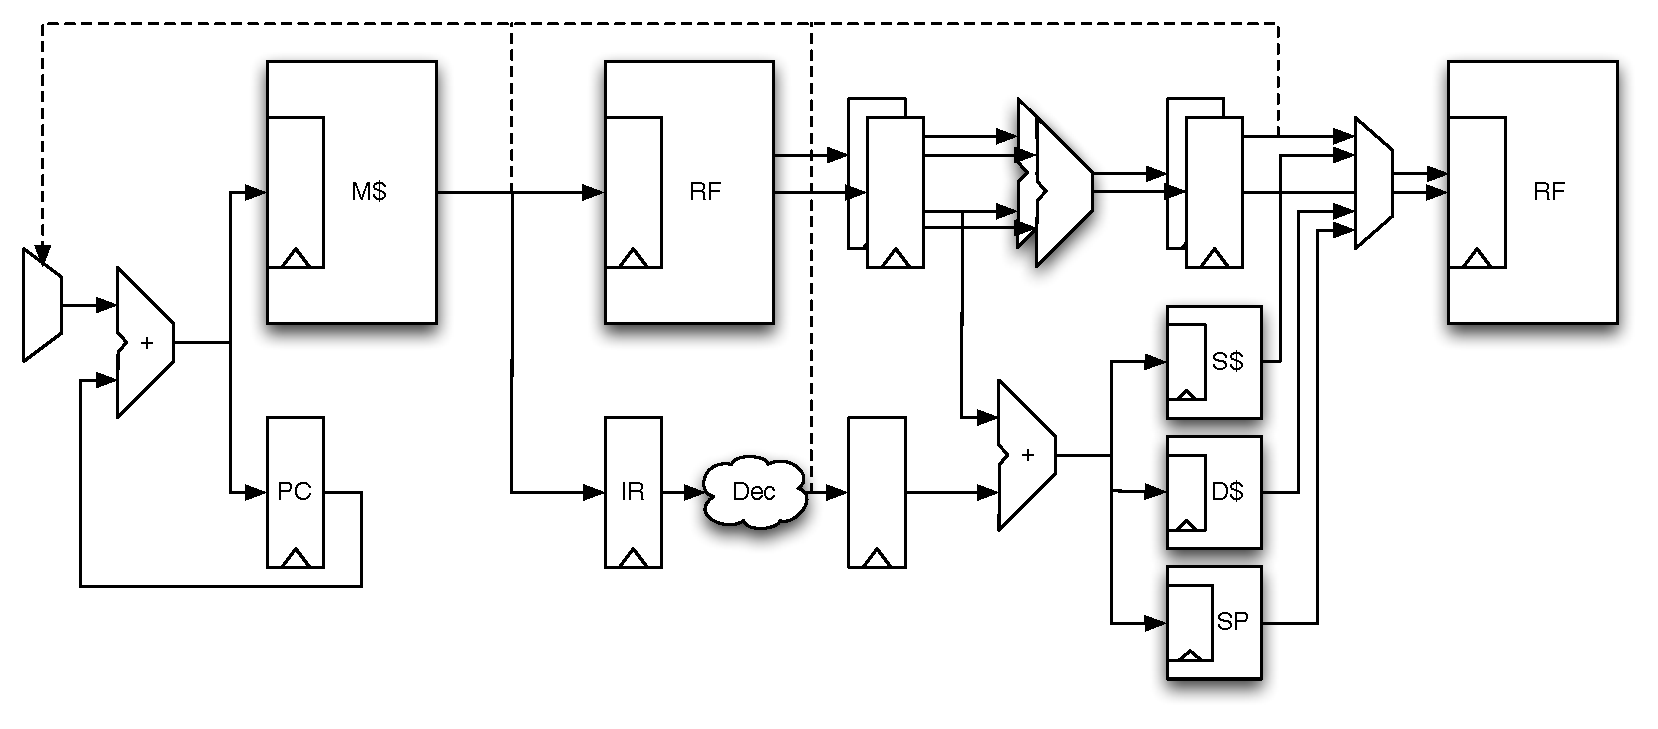
\includegraphics[width=\textwidth]{fig/pipeline}
    \caption{Pipeline of Patmos with fetch, decode, execute, memory, and write back stages.}\label{fig:pipeline}
\end{figure}


\section{Register Files}

The register files available in Patmos are depicted by
Figure~\ref{fig:registers}. In short, Patmos offers:
\begin{itemize}
  \item 32, 32-bit general-purpose registers (\texttt{R}) : \texttt{r0}, \ldots, \texttt{r31} \\
    \texttt{r0} is read-only, set to zero (\texttt{0}).
  \item 8, single-bit predicate registers (\texttt{P}): \texttt{p0}, \ldots, \texttt{p7}, \\
    \texttt{p0} is read-only, set to \texttt{true} (\texttt{1}).
  \item 16, 32-bit special-purpose registers (\texttt{S}): \texttt{s0}, \ldots, \texttt{s15}
\end{itemize}

The general-purpose registers \texttt{R} are read in the \code{DEC} stage
and written in the \code{WB} stage. Full forwarding makes them available
in the \code{EX} stage before written into the register file.

The predicate registers are single bits that are set and read in the \code{EX}
stage.

The special registers \code{S} is just a collection of various `special'
processor registers. These registers might be used by different units/stages
in the pipeline and are not physically collected in a `register file'.
The pipeline stage where those registers are read and written by the
\code{mfs} and \code{mts} are dependent on the type of the special
register.

\martin{The three `register' files shall constitute the state of the processor.
Every non-obvious register, such as method base, shall be mapped to a
`special' register. Even the current PC on an interrupt shall end up in a
register that is mapped into the special register domain.}

\stefan{Umm .. it would be really good to define somewhere in which stages which special register is actually read or written by mfs/mts
;).}

So all-in-all the recoverable process state is: general-purpose registers
\code{R}, the predicates \code{P}, and a collection of various processor
registers mapped to the `special' register files \code{S}.

Concurrently writing and reading the same register in the same cycle
will, for the read, yield the old value of the register. Reads in
subsequent cycles return the result most recently written to the
register, i.e., the pipeline implements full forwarding.

When writing concurrently to the same register, the result is
undefined. If two instructions of the current bundle have the same
destination register, the result is only defined if the predicate of
at most one instruction in the bundle evaluates to \texttt{true} (1).

\wolf{In practice, the result is even defined if both instructions
  write to the same register, but I would not make this a feature of
  the ISA.}

The predicate registers are usually encoded as $4$-bit operands, where the most
significant bit indicates that the value read from the register file should be
inverted before it is used. For operands that are written, this additional bit
is omitted.

The special-purpose registers of \texttt{S} allow access to some dedicated
registers:
\begin{itemize}
  \item The lower $8$ bits of \texttt{s0} can be used to save/restore
    \emph{all} predicate registers at once. The other bits of that
    register are currently reserved, but not used. Setting the reserved 
	bits has no effect.
  \item \texttt{s1} can also be accessed through the name \texttt{sm} and
    represents the result of a decoupled load operation. The value is
    already sign-/zero-extended according to the load instruction. 
  \item \texttt{s2} and \texttt{s3} can also be accessed through the names
    \texttt{sl} and \texttt{sh} and represent the lower and upper
    32-bits a multiplication. 
  \item \texttt{s5} can also be accessed through the name \texttt{ss} and 
    represents the register pointing to the top of the saved stack 
	content in the main memory (i.e., the current stack spill pointer).
	Updating \texttt{s5} does not change \texttt{s6} or spill the stack cache.
  \item \texttt{s6} can also be accessed through the name \texttt{st} and
    represents a pointer to the top-most element of the content of the
    stack cache. 
	Updating \texttt{s6} does not change \texttt{s5} or spill the stack cache.
\end{itemize}

\stefan{None of the registers should be read-only, as they need to be restored when
we switch contexts.}

\begin{figure}[p]

  \begin{multicols}{2}
    \centering

    \subfloat[\label{fig:registers:r}General-Purpose Registers (\texttt{R})]{
      \begin{bytefield}[bitwidth=.59em]{32}
        \bitheader{0-31} \\
        \bitbox{32}{r0 (zero, read-only)} \\
        \bitbox{32}{r1 (result, scratch)} \\
        \bitbox{32}{r2 (result 64-bit, scratch)} \\
        \bitbox{32}{r3 (argument 1, scratch)} \\
        \bitbox{32}{r4 (argument 2, scratch)} \\
        \bitbox{32}{r5 (argument 3, scratch)} \\
        \bitbox{32}{r6 (argument 4, scratch)} \\
        \bitbox{32}{r7 (argument 5, scratch)} \\
        \bitbox{32}{r8 (argument 6, scratch)} \\ \bitbox{32}{r9 (scratch)} \\
        \bitbox{32}{r10 (scratch)} \\ \bitbox{32}{r11 (scratch)} \\
        \bitbox{32}{r12 (scratch)} \\ \bitbox{32}{r13 (scratch)} \\
        \bitbox{32}{r14 (scratch)} \\ \bitbox{32}{r15 (scratch)} \\
        \bitbox{32}{r16 (scratch)} \\ \bitbox{32}{r17 (scratch)} \\
        \bitbox{32}{r18 (scratch)} \\ \bitbox{32}{r19 (scratch)} \\
        \bitbox{32}{r20 (saved)} \\ \bitbox{32}{r21 (saved)} \\
        \bitbox{32}{r22 (saved)} \\ \bitbox{32}{r23 (saved)} \\
        \bitbox{32}{r24 (saved)} \\ \bitbox{32}{r25 (saved)} \\
        \bitbox{32}{r26 (saved)} \\
        \bitbox{32}{r27 (temp.\ register, saved)} \\
        \bitbox{32}{r28 (frame pointer, saved)} \\
        \bitbox{32}{r29 (stack pointer, saved)} \\
        \bitbox{32}{r30 (function base, saved)} \\
        \bitbox{32}{r31 (function offset, saved)} \\
      \end{bytefield}
    }

    \newpage

    \vspace*{\stretch{1}}

    \subfloat[\label{fig:registers:pr}Predicate Registers (\texttt{P})]{
      \newcommand{\bitlabel}[1]{
        \bitbox[]{1}{\raisebox{0pt}[5ex][1pt]{\turnbox{45}{\fontsize{7}{7}\selectfont#1}}}
      }
      \begin{bytefield}[bitwidth=1.5em]{8}
        \bitlabel{p7} \bitlabel{p6} \bitlabel{p5} \bitlabel{p4}
        \bitlabel{p3} \bitlabel{p2} \bitlabel{p1} \bitlabel{p0 -- Read only, always \texttt{1}} \\
        \bitheader{0-7} \\
        \bitbox{1}{} \bitbox{1}{} \bitbox{1}{} \bitbox{1}{}
        \bitbox{1}{} \bitbox{1}{} \bitbox{1}{} \bitbox{1}{} \\
      \end{bytefield}
    }

    \vspace*{\stretch{2}}

    \subfloat[\label{fig:registers:s}Special-Purpose Registers (\texttt{S})]{
      \begin{bytefield}[bitwidth=.59em]{32}
        \bitheader{0-31} \\
        \bitbox{24}{reserved} \bitbox{8}{p7 \dots p0} \bitbox[]{4}{s0} \\
        \bitbox{32}{sm (load result)} \bitbox[]{4}{s1} \\
        \bitbox{32}{sl (mul low)} \bitbox[]{4}{s2} \\
        \bitbox{32}{sh (mul high)} \bitbox[]{4}{s3} \\
        \bitbox{32}{s4} \\
        \bitbox{32}{ss (spill pointer)} \bitbox[]{4}{s5} \\
        \bitbox{32}{st (stack pointer)} \bitbox[]{4}{s6} \\
        \bitbox{32}{s7} \\ \bitbox{32}{s8} \\
        \bitbox{32}{s9} \\ \bitbox{32}{s10} \\ \bitbox{32}{s11} \\
        \bitbox{32}{s12} \\ \bitbox{32}{s13} \\ \bitbox{32}{s14} \\ \bitbox{32}{s15} \\
      \end{bytefield}
    }

    \vspace*{\stretch{4}}~

  \end{multicols}

  \caption{General-purpose register file, predicate registers, and
           special-purpose registers of Patmos.}
  \label{fig:registers}
\end{figure}

\section{Bundle Formats}

All Patmos instructions are 32 bits wide and are structured according to
one of the instruction formats defined in the following section. Up to two
instructions can be combined to form an instruction bundle; Patmos bundles are
thus either 32 or 64 bits wide. The bundles sizes are recognized by the value of
the most significant bit, where $0$ indicates a short, 32-bit bundle and $1$ a
long, 64-bit bundle.

The following figures illustrate these two bundle variants:
\begin{itemize}
 \item 32-bit bundle format\\[2ex]
   \begin{bytefield}{32}
     \bitheader{0-31} \\
     \bitbox{1}{0} & \bitbox{31}{\bitssubclass} \\
   \end{bytefield}

 \item 64-bit bundle format \\[2ex]
   \begin{bytefield}[lsb=32]{32} \bitheader{32-63} \\
     \bitbox{1}{1} & \bitbox{31}{\bitssubclass} \\
   \end{bytefield}
   \hspace{.5em}
   \begin{bytefield}{32} \bitheader{0-31} \\
     \bitbox{1}{x} & \bitbox{31}{\bitssubclass} \\
   \end{bytefield}
\end{itemize}

\section{Instruction Formats}

This section gives an overview of all instruction formats defined in the Patmos
ISA. Individual instructions of the various formats are defined in the next
section. Gray fields indicate bits whose function is determined by a sub-class
of the instruction format. Black fields are not used.

\begin{itemize}
  \item ALUi -- Arithmetic Immediate \\[2ex]
    \begin{bytefield}{32}
      \bitheader{0-31} \\
      \bitbox{1}{x} & \bitbox{4}{Pred} & \bitbox{2}{00} & \bitbox{3}{Func} &
      \bitbox{5}{Rd} & \bitbox{5}{Rs1} & \bitbox{12}{Immediate} \\
    \end{bytefield}
  \item ALUl -- Long Immediate \\[2ex]
    \begin{bytefield}{32} 
      \bitheader{0-31} \\
      \bitbox{1}{1} & \bitbox{4}{Pred} & \bitbox{5}{11111} &
      \bitbox{5}{Rd} & \bitbox{5}{Rs1} & \bitbox{5}{\bitsunused} &
      \bitbox{3}{000} & \bitbox{4}{Func} \\
      \bitheader{0-31} \\ 
      \bitbox{32}{Long Immediate} \\
    \end{bytefield}
  \item ALU -- Arithmetic \\[2ex]
        \begin{bytefield}{32}
          \bitheader{0-31} \\
          \bitbox{1}{x} & \bitbox{4}{Pred} & \bitbox{5}{01000} &
          \bitbox{15}{\bitssubclass} &
          \bitbox{3}{Opc} & \bitbox{4}{Func} \\
        \end{bytefield}

        \begin{bytefield}[leftcurly=.]{32}
          \begin{leftwordgroup}{\parbox{8em}{ALUr -- Register}}
            \bitheader{0-31} \\
            \bitbox{1}{x} & \bitbox{4}{Pred} & \bitbox{5}{01000} &
            \bitbox{5}{Rd} & \bitbox{5}{Rs1} & \bitbox{5}{Rs2} &
            \bitbox{3}{000} & \bitbox{4}{Func}
          \end{leftwordgroup} \\
          \begin{leftwordgroup}{\parbox{8em}{ALUm -- Multiply}}
            \bitheader{0-31} \\
            \bitbox{1}{x} & \bitbox{4}{Pred} & \bitbox{5}{01000} &
            \bitbox{5}{\bitsunused} & \bitbox{5}{Rs1} & \bitbox{5}{Rs2} &
            \bitbox{3}{010} & \bitbox{4}{Func}
          \end{leftwordgroup} \\
          \begin{leftwordgroup}{\parbox{8em}{ALUc -- Compare}}
            \bitheader{0-31} \\
            \bitbox{1}{x} & \bitbox{4}{Pred} & \bitbox{5}{01000} &
            \bitbox{2}{\bitsunused} & \bitbox{3}{Pd} & \bitbox{5}{Rs1} & \bitbox{5}{Rs2} &
            \bitbox{3}{011} & \bitbox{4}{Func}
          \end{leftwordgroup} \\
          \begin{leftwordgroup}{\parbox{8em}{ALUp -- Predicate}}
            \bitheader{0-31} \\
            \bitbox{1}{x} & \bitbox{4}{Pred} & \bitbox{5}{01000} &
            \bitbox{2}{\bitsunused} & \bitbox{3}{Pd} & \bitbox{1}{\bitsunused} & \bitbox{4}{Ps1} & \bitbox{1}{\bitsunused} & \bitbox{4}{Ps2} &
            \bitbox{3}{100} & \bitbox{4}{Func}
          \end{leftwordgroup} \\
          %% \begin{leftwordgroup}{\parbox{8em}{Unused}}
          %%   \bitheader{0-31} \\
          %%   \bitbox{1}{x} & \bitbox{4}{Pred} & \bitbox{5}{01000} &
          %%   \bitbox{15}{\bitssubclass} &
          %%   \bitbox{3}{001} & \bitbox{4}{Func}
          %% \end{leftwordgroup} \\
          %% \begin{leftwordgroup}{\parbox{8em}{Unused}}
          %%   \bitheader{0-31} \\
          %%   \bitbox{1}{x} & \bitbox{4}{Pred} & \bitbox{5}{01000} &
          %%   \bitbox{15}{\bitssubclass} &
          %%   \bitbox{3}{101} & \bitbox{4}{Func}
          %% \end{leftwordgroup} \\
          %% \begin{leftwordgroup}{\parbox{8em}{Unused}}
          %%   \bitheader{0-31} \\
          %%   \bitbox{1}{x} & \bitbox{4}{Pred} & \bitbox{5}{01000} &
          %%   \bitbox{15}{\bitssubclass} &
          %%   \bitbox{3}{110} & \bitbox{4}{Func}
          %% \end{leftwordgroup} \\
          %% \begin{leftwordgroup}{\parbox{8em}{Unused}}
          %%   \bitheader{0-31} \\
          %%   \bitbox{1}{x} & \bitbox{4}{Pred} & \bitbox{5}{01000} &
          %%   \bitbox{15}{\bitssubclass} &
          %%   \bitbox{3}{111} & \bitbox{4}{Func}
          \end{leftwordgroup} \\
        \end{bytefield}

  \item SPC -- Special \\[2ex]
        \begin{bytefield}{32}
          \bitheader{0-31} \\
          \bitbox{1}{x} & \bitbox{4}{Pred} & \bitbox{5}{01001} &
          \bitbox{15}{\bitssubclass} &
          \bitbox{3}{Opc} & \bitbox{4}{I/R/F} \\
        \end{bytefield}

        \begin{bytefield}[leftcurly=.]{32}
          \begin{leftwordgroup}{\parbox{11em}{SPCw -- Wait}}
            \bitheader{0-31} \\
            \bitbox{1}{x} & \bitbox{4}{Pred} & \bitbox{5}{01001} &
            \bitbox{15}{\bitsunused} &
            \bitbox{3}{001} & \bitbox{4}{Func}
          \end{leftwordgroup} \\
          \begin{leftwordgroup}{\parbox{11em}{SPCt -- Move To Special}}
            \bitheader{0-31} \\
            \bitbox{1}{x} & \bitbox{4}{Pred} & \bitbox{5}{01001} &
            \bitbox{5}{\bitsunused} & \bitbox{5}{Rs1} & \bitbox{5}{\bitsunused} &
            \bitbox{3}{010} & \bitbox{4}{Sd}
          \end{leftwordgroup} \\
          \begin{leftwordgroup}{\parbox{11em}{SPCf -- Move From Special}}
            \bitheader{0-31} \\
            \bitbox{1}{x} & \bitbox{4}{Pred} & \bitbox{5}{01001} &
            \bitbox{5}{Rd} & \bitbox{10}{\bitsunused} &
            \bitbox{3}{011} & \bitbox{4}{Ss}
          \end{leftwordgroup} \\
          %% \begin{leftwordgroup}{\parbox{11em}{Unused}}
          %%   \bitheader{0-31} \\
          %%   \bitbox{1}{x} & \bitbox{4}{Pred} & \bitbox{5}{01001} &
          %%   \bitbox{15}{\bitssubclass} &
          %%   \bitbox{3}{000} & \bitbox{4}{I/R/F}
          %% \end{leftwordgroup} \\
          %% \begin{leftwordgroup}{\parbox{11em}{Unused}}
          %%   \bitheader{0-31} \\
          %%   \bitbox{1}{x} & \bitbox{4}{Pred} & \bitbox{5}{01001} & 
          %%   \bitbox{15}{\bitssubclass} &
          %%   \bitbox{3}{100} & \bitbox{4}{I/R/F}
          %% \end{leftwordgroup} \\
          %% \begin{leftwordgroup}{\parbox{11em}{Unused}}
          %%   \bitheader{0-31} \\
          %%   \bitbox{1}{x} & \bitbox{4}{Pred} & \bitbox{5}{01001} &
          %%   \bitbox{15}{\bitssubclass} &
          %%   \bitbox{3}{101} & \bitbox{4}{I/R/F}
          %% \end{leftwordgroup} \\
          %% \begin{leftwordgroup}{\parbox{11em}{Unused}}
          %%   \bitheader{0-31} \\
          %%   \bitbox{1}{x} & \bitbox{4}{Pred} & \bitbox{5}{01001} &
          %%   \bitbox{15}{\bitssubclass} &
          %%   \bitbox{3}{110} & \bitbox{4}{I/R/F}
          %% \end{leftwordgroup} \\
          %% \begin{leftwordgroup}{\parbox{11em}{Unused}}
          %%   \bitheader{0-31} \\
          %%   \bitbox{1}{x} & \bitbox{4}{Pred} & \bitbox{5}{01001} &
          %%   \bitbox{15}{\bitssubclass} &
          %%   \bitbox{3}{111} & \bitbox{4}{I/R/F}
          %% \end{leftwordgroup}
        \end{bytefield}

  \item LDT -- Load Typed \\[2ex]
        \begin{bytefield}{32}
          \bitheader{0-31} \\
          \bitbox{1}{x} & \bitbox{4}{Pred} & \bitbox{5}{01010} &
          \bitbox{5}{Rd} & \bitbox{5}{Ra} & \bitbox{5}{Type} & \bitbox{7}{Offset} \\
        \end{bytefield}
  \item STT -- Store Typed \\[2ex]
        \begin{bytefield}{32}
          \bitheader{0-31} \\
          \bitbox{1}{x} & \bitbox{4}{Pred} & \bitbox{5}{01011} &
          \bitbox{5}{Type} & \bitbox{5}{Ra} & \bitbox{5}{Rs} & \bitbox{7}{Offset} \\
        \end{bytefield}

  \item STC -- Stack Control \\[2ex]
        \begin{bytefield}{32}
          \bitheader{0-31} \\
          \bitbox{1}{x} & \bitbox{4}{Pred} & \bitbox{5}{01100} &
          \bitbox{2}{Op} & \bitbox{2}{F} & \bitbox{18}{\bitssubclass} \\
        \end{bytefield}

        \begin{bytefield}[leftcurly=.]{32}
          \begin{leftwordgroup}{\parbox{13em}{STCi -- Stack Control Immediate}}
            \bitheader{0-31} \\
            \bitbox{1}{x} & \bitbox{4}{Pred} & \bitbox{5}{01100} &
            \bitbox{2}{Op} & \bitbox{2}{00} &
            \bitbox{18}{Immediate}
          \end{leftwordgroup} \\
          \begin{leftwordgroup}{\parbox{13em}{STCr -- Stack Control Register}}
            \bitheader{0-31} \\
            \bitbox{1}{x} & \bitbox{4}{Pred} & \bitbox{5}{01100} &
            \bitbox{2}{Op} & \bitbox{2}{01} &
            \bitbox{1}{\bitsunused} & \bitbox{5}{Rs} & \bitbox{12}{\bitsunused}
          \end{leftwordgroup}
        \end{bytefield}

  \item CFL -- Control Flow \\[2ex]
        \begin{bytefield}{32}
          \bitheader{0-31} \\
          \bitbox{1}{x} & \bitbox{4}{Pred} & \bitbox{3}{11x} & \bitbox{2}{Op} &
          \bitbox{22}{\bitssubclass} \\
        \end{bytefield}

        \begin{bytefield}[leftcurly=.]{32}
          \begin{leftwordgroup}{\parbox{12em}{CFLb -- Call / Branch}}
            \bitheader{0-31} \\
            \bitbox{1}{x} & \bitbox{4}{Pred} & \bitbox{3}{110} & \bitbox{2}{Op} &
            \bitbox{22}{Immediate}
          \end{leftwordgroup} \\
          \begin{leftwordgroup}{\parbox{12em}{CFLi -- Call / Branch Indirect}}
            \bitheader{0-31} \\
            \bitbox{1}{x} & \bitbox{4}{Pred} & \bitbox{3}{111} & \bitbox{2}{00} & 
            \bitbox{5}{\bitsunused} & \bitbox{5}{Rs1} & \bitbox{8}{\bitsunused} & \bitbox{4}{Op}
          \end{leftwordgroup} \\
          \begin{leftwordgroup}{\parbox{12em}{CFLr -- Return}}
            \bitheader{0-31} \\
            \bitbox{1}{x} & \bitbox{4}{Pred} & \bitbox{3}{111} & \bitbox{2}{10} &
            \bitbox{5}{\bitsunused} & \bitbox{5}{Rb} & \bitbox{5}{Ro} & \bitbox{3}{\bitsunused} &\bitbox{4}{Op}
          \end{leftwordgroup} \\
          \begin{leftwordgroup}{\parbox{12em}{Reserved}}
            \bitheader{0-31} \\
            \bitbox{1}{x} & \bitbox{4}{Pred} & \bitbox{3}{111} & \bitbox{2}{11} &
            \bitbox{22}{\bitssubclass}
          \end{leftwordgroup} \\
        \end{bytefield}
\end{itemize}

\clearpage
\section{Instruction Opcodes}
\label{sec:instruction_opcodes}

This section defines the instruction set architecture, the instruction opcodes,
and the behavior of the respective instructions of Patmos. This section should
be less used for discussions and should slowly converge to a final definition
of the instruction set.

\subsection{Binary Arithmetic}

Applies to the ALUr, ALUi, and ALUl formats.  Operand \texttt{Op2}
denotes either the \texttt{Rs2}, or the \texttt{Immediate} operand, or
the \texttt{Long Immediate}. The immediate operand is zero-extended.  For
shift and rotate operations, only the lower $5$ bits of the operand
are considered. Table~\ref{tab:alufunc} shows the encoding of the
\texttt{func} field; for ALUi instructions, only functions in the
upper half of that table are available.

\begin{itemize}
  \item ALUr -- Register \\[2ex]
    \begin{bytefield}{32}
      \bitheader{0-31} \\
      \bitbox{1}{x} & \bitbox{4}{Pred} & \bitbox{5}{01000} &
      \bitbox{5}{Rd} & \bitbox{5}{Rs1} & \bitbox{5}{Rs2} &
      \bitbox{3}{000} & \bitbox{4}{Func} \\
    \end{bytefield}
  \item ALUi -- Arithmetic Immediate \\[2ex]
    \begin{bytefield}{32}
      \bitheader{0-31} \\
      \bitbox{1}{x} & \bitbox{4}{Pred} & \bitbox{2}{00} & \bitbox{3}{Func} &
      \bitbox{5}{Rd} & \bitbox{5}{Rs1} & \bitbox{12}{Immediate} \\
    \end{bytefield}
  \item ALUl -- Long Immediate\\[2ex]
    \begin{bytefield}{32}
      \bitheader{0-31} \\
      \bitbox{1}{1} & \bitbox{4}{Pred} & \bitbox{5}{11111} &
      \bitbox{5}{Rd} & \bitbox{5}{Rs1} & \bitbox{5}{\bitsunused} & 
      \bitbox{3}{000} & \bitbox{4}{Func} \\
      \bitheader{0-31} \\ 
      \bitbox{32}{Long Immediate} \\
   \end{bytefield}
\end{itemize}

\begin{table}[hb]
  \centering
  \begin{tabular}{lll}
    \toprule
    Func & Name   & Semantics \\
    \midrule
    0000 & add    & \texttt{Rd = Rs1 + Op2} \\
    0001 & sub    & \texttt{Rd = Rs1 - Op2} \\
    0010 & xor    & \texttt{Rd = Rs1 \XOR Op2} \\
    0011 & sl     & \texttt{Rd = Rs1 \shl Op2$_{[0:4]}$} \\
    0100 & sr     & \texttt{Rd = Rs1 \shr Op2$_{[0:4]}$} \\
    0101 & sra    & \texttt{Rd = Rs1 \ashr Op2$_{[0:4]}$} \\
    0110 & or     & \texttt{Rd = Rs1 \OR Op2} \\
    0111 & and    & \texttt{Rd = Rs1 \AND Op2} \\
    \cmidrule{1-3}
    1000 & ---	& unused \\
    1001 & ---    & unused \\
    1010 & ---    & unused \\
    1011 & nor    & \texttt{Rd = \NOT (Rs1 \OR Op2)} \\
    1100 & shadd  & \texttt{Rd = (Rs1 \shl 1) + Op2} \\
    1101 & shadd2 & \texttt{Rd = (Rs1 \shl 2) + Op2} \\
    1110 & ---    & unused \\
    1111 & ---    & unused \\
    \bottomrule
  \end{tabular}
  \caption{General ALU functions}
  \label{tab:alufunc}
\end{table}

\paragraph{Pseudo Instructions}
\begin{itemize}
  \item \texttt{mov Rd = Rs}~\dots~\texttt{add Rd = Rs + 0}
  \item \texttt{clr Rd}~\dots~\texttt{add Rd = r0 + 0}
  \item \texttt{neg Rd = -Rs}~\dots~\texttt{sub Rd = 0 - Rs}
  \item \texttt{not Rd = \NOT Rs}~\dots~\texttt{nor Rd = \NOT (Rs \OR R0)}
  \item \texttt{li Rd = Immediate}~\dots~\texttt{add Rd = r0 + Immediate}
  \item \texttt{li Rd = Immediate}~\dots~\texttt{sub Rd = r0 - Immediate}
  \item \texttt{nop}~\dots~\texttt{sub r0 = r0 - 0}
\end{itemize}


\paragraph{Note}
The use of \texttt{sub r0 = r0 - 0} to encode a \texttt{nop}
pseudo-instruction results in a value of \texttt{0x00400000} in the
binary instruction stream. This helps in distinguishing the execution
of compiler-generated \texttt{nops} from executing instructions from
memory that happens to be zero.

\clearpage
\subsection{Multiply}

Applies to the ALUm format only. Multiplications are executed in
parallel with the regular pipeline and finish within a fixed number of
cycles \todo{how many?}. Table~\ref{tab:mulfunc} shows the encoding of
the \texttt{func} field for the ALUm instruction format.

\begin{itemize}
  \item ALUm -- Multiply \\[2ex]
    \begin{bytefield}{32}
      \bitheader{0-31} \\
      \bitbox{1}{x} & \bitbox{4}{Pred} & \bitbox{5}{01000} &
      \bitbox{5}{\bitsunused} & \bitbox{5}{Rs1} & \bitbox{5}{Rs2} &
      \bitbox{3}{010} & \bitbox{4}{Func} \\
    \end{bytefield}
\end{itemize}

\begin{table}[hb]
  \centering
  \begin{tabular}{lll}
    \toprule
    Func & Name   & Semantics \\
    \midrule
    0000 & mul    & \texttt{sl = Rs1 * Rs2;}\\
         &        & \texttt{sh = (Rs1 * Rs2) \shr 32} \\
    0001 & mulu   & \texttt{sl = (uint32\_t)Rs1 * (uint32\_t)Rs2;} \\
         &        & \texttt{sh = ((uint32\_t)Rs1 * (uint32\_t)Rs2) \shr 32} \\
    0010 & ---    & unused \\
    \dots& \dots  & \dots \\
    1111 & ---    & unused \\
    \bottomrule
  \end{tabular}
  \caption{Multiplication functions}
  \label{tab:mulfunc}
\end{table}


\paragraph{Behavior}

Perform multiplication in multiple cycles and write the result into
destination registers \texttt{sl} and \texttt{sh}.

\paragraph{Note}

Multiplications are pipelined, it is thus possible to issue one multiplication on
every cycles. Multiplications can only be issued in the first slot. 

\stefan{Not yet final. 64bit support and the special registers for multiply might 
vanish. Maybe merge mul and mulu into the ALU Func field somehow to kill off the ALUm format? 
We could keep the special register to access the high word and write the low
word into a GPR when using ALUl format, so we save one mfs per mul.
(remove this comment when multiply ISA is (somewhat) finalized)}

\clearpage
\subsection{Compare}

Applies to the ALUc format only. Table~\ref{tab:cmpfunc} shows the
encoding of the \texttt{func} field for the ALUc format.

\begin{itemize}
  \item ALUc -- Compare \\[2ex]
    \begin{bytefield}{32}
      \bitheader{0-31} \\
      \bitbox{1}{x} & \bitbox{4}{Pred} & \bitbox{5}{01000} &
      \bitbox{2}{\bitsunused} & \bitbox{3}{Pd} & \bitbox{5}{Rs1} & \bitbox{5}{Rs2} &
      \bitbox{3}{011} & \bitbox{4}{Func} \\
    \end{bytefield}
\end{itemize}

\begin{table}[hb]
  \centering
  \begin{tabular}{lll}
    \toprule
    Func & Name   & Semantics \\
    \midrule
    0000 & cmpeq  & \texttt{Pd = Rs1 ==  Rs2} \\
    0001 & cmpneq & \texttt{Pd = Rs1 !=  Rs2} \\
    0010 & cmplt  & \texttt{Pd = Rs1 \textless\ Rs2} \\
    0011 & cmple  & \texttt{Pd = Rs1 \textless= Rs2} \\
    0100 & cmpult & \texttt{Pd = Rs1 \textless\ Rs2, unsigned} \\
    0101 & cmpule & \texttt{Pd = Rs1 \textless= Rs2, unsigned} \\
    0110 & btest  & \texttt{Pd = (Rs1 \AND (1 \shl Rs2)) != 0} \\
    0111 & ---    & unused \\
    \dots& \dots  & \dots \\
    1111 & ---    & unused \\
    \bottomrule
  \end{tabular}
  \caption{Compare functions}
  \label{tab:cmpfunc}
\end{table}

\paragraph{Pseudo Instructions}
\begin{itemize}
  \item \texttt{isodd Pd = Rs1}~\dots~\texttt{btest Pd = Rs1[r0]}
  \item \texttt{mov Pd = Rs}~\dots~\texttt{cmpneq Pd = Rs != r0}
\end{itemize}

\paragraph{Note}

The predicate register is read and written in the execute stage.

\stefan{We discussed about adding short immediate versions, but with the current predicate handling this is not
a trivial change for the compiler, so we skip that. Instead, we might introduce bez/bnez instructions, which is much more common anyway.}

\clearpage
\subsection{Predicate}

Applies to the ALUp format only, the opcodes correspond to those of
the ALU operations on general purpose
registers. Table~\ref{tab:predfunc} shows the encoding of the
\texttt{func} field for the ALUp format.

\martin{Why do we have this encoding of predicate operations with empty function
codes in-between? No need to be `compatible' with ALU operations, just makes decoding
a little bit more complex.}

\begin{itemize}
  \item ALUp -- Predicate \\[2ex]
    \begin{bytefield}{32}
      \bitheader{0-31} \\
      \bitbox{1}{x} & \bitbox{4}{Pred} & \bitbox{5}{01000} &
      \bitbox{2}{\bitsunused} & \bitbox{3}{Pd} & \bitbox{1}{\bitsunused} & \bitbox{4}{Ps1} & \bitbox{1}{\bitsunused} & \bitbox{4}{Ps2} &
      \bitbox{3}{100} & \bitbox{4}{Func} \\
    \end{bytefield}
\end{itemize}

\begin{table}[hb]
  \centering
  \begin{tabular}{lll}
    \toprule
    Func & Name   & Semantics \\
    \midrule
    0000 & ---    & unused \\
    \dots& \dots  & \dots \\
    0101 & ---    & unused \\
    0110 & por     & \texttt{Pd = Ps1 \OR Ps2} \\
    0111 & pand    & \texttt{Pd = Ps1 \AND Ps2} \\
    1000 & ---    & unused \\
    1001 & ---    & unused \\
    1010 & pxor    & \texttt{Pd = Ps1 \XOR Ps2} \\
    1011 & ---    & unused \\
    \dots& \dots  & \dots \\
    1111 & ---    & unused \\
    \bottomrule
  \end{tabular}
  \caption{Predicate functions}
  \label{tab:predfunc}
\end{table}

\paragraph{Pseudo Instructions}
\begin{itemize}
  \item \texttt{pmov Pd = Ps}~\dots~\texttt{por Pd = Ps \OR Ps}
  \item \texttt{pnot Pd = \NOT Ps}~\dots~\texttt{pxor Pd = (Ps \XOR p0)}
  \item \texttt{pset Pd = 1}~\dots~\texttt{por Pd = p0 \OR p0}
  \item \texttt{pclr Pd = 0}~\dots~\texttt{pxor Pd = p0 \XOR p0}
\end{itemize}

\paragraph{Note}
The predicate register is read and written in the execute stage.
All predicate combine instruction mnemonics (including pseudo instructions) are prefixed with \texttt{p}, 
all other instructions involving predicates are not prefixed (e.g., moving from register to predicate).

\stefan{We have a mov with two registers (\texttt{add}), mov with two predicates (\texttt{por}), a mov from register to
predicate (\texttt{cmpnez}), as well as mov from register bit to predicate (\texttt{btest}), but we are missing a 
mov from predicate to register (is now a predicated set and predicated clr), and mov from predicate to register bit (is now done with
bitmasks).}

%Applies to the SPCn format only. Issue \texttt{Imm} NOP
%operations to the pipeline. The main idea is to save code size, however, the
%multi-cycle NOP might also be used to enforce certain timing constraints, e.g.,
%wait for a certain amount of time, ensure a minimal execution time, et cetera.
%
%\begin{itemize}
%  \item SPCn -- NOP \\[2ex]
%        \begin{bytefield}{32} \bitheader{0-31}\\ \bitbox{1}{x} & \bitbox{4}{Pred} & \bitbox{5}{01001} & \bitbox{15}{\bitsunused} & \bitbox{3}{000} & \bitbox{4}{Imm} \end{bytefield}\\
%\end{itemize}
%
%\paragraph{Behavior}
%\begin{itemize}
%  \item[\texttt{IF}] --
%  \item[\texttt{DR}] Read register operands \texttt{Pred}.\\
%                     \texttt{tmp} = \texttt{Pred} ? \texttt{Imm} : 0. \\
%                     while (\texttt{tmp}-\,- != 0) \{ stall \texttt{DR}; next cycle; \}
%  \item[\texttt{EX}] --
%  \item[\texttt{MW}] --
%\end{itemize}
%
%\paragraph{Note}
%
%A NOP can only be issued at the first position within a bundle. This does in no
%way restrict the use of the NOP. It can always be scheduled in the next/previous
%bundle, while incrementing/decrementing the number of NOP cycles accordingly;
%the code size is in both cases not increased.

\clearpage
\subsection{Wait}

Applies to the SPCw format only. Wait for a multiplication or memory
operation to complete by stalling the
pipeline. Table~\ref{tab:waitfunc} shows the encoding of the
\code{func} field.

\begin{itemize}
  \item SPCw -- Wait \\[2ex]
    \begin{bytefield}{32}
      \bitheader{0-31} \\
      \bitbox{1}{x} & \bitbox{4}{Pred} & \bitbox{5}{01001} &
      \bitbox{15}{\bitsunused} &
      \bitbox{3}{001} & \bitbox{4}{Func} \\
    \end{bytefield}
\end{itemize}

\begin{table}[hb]
  \centering
  \begin{tabular}{lll}
    \toprule
    Func & Name     & Semantics \\
    \midrule
    0000 & wait.mem & Wait for a memory access \\
    0001 & ---    & unused \\
    \dots& \dots  & \dots \\
    1111 & ---    & unused \\
    \bottomrule
  \end{tabular}
  \caption{Wait function encoding}
  \label{tab:waitfunc}
\end{table}

\paragraph{Note}

A Wait can only be issued at the first position within a bundle.
This instruction is not (yet) implemented in hardware as we do not
(yet) support split loads. \martin{And maybe we will never do as
the gain is not worth the effort.}

\clearpage
\subsection{Move To Special}

Applies to the SPCt format only. Copy the value of a general-purpose
register to a special-purpose register. The only instruction is
\texttt{mts}, which stores the content of general-purpose register
\texttt{Rs1} in special register \texttt{Sd}.

\begin{itemize}
  \item SPCt -- Move To Special \\[2ex]
    \begin{bytefield}{32}
      \bitheader{0-31} \\
      \bitbox{1}{x} & \bitbox{4}{Pred} & \bitbox{5}{01001} &
      \bitbox{5}{\bitsunused} & \bitbox{5}{Rs1} & \bitbox{5}{\bitsunused} &
      \bitbox{3}{010} & \bitbox{4}{Sd} \\
    \end{bytefield}
\end{itemize}



\paragraph{Note}



Special registers \texttt{sm}, \texttt{sl}, \texttt{sh} are read-only, writing
to those registers may result in undefined behavior.

\stefan{What should we do in case of a context switch? We would either need to restart the last load and multiply, or restore all special registers..}
\martin{Restart sounds problematic. I would say the special registers are part of the context and need to be saved and
than writable.}

\wolf{Saving \texttt{sm} can be faked by storing the contents of
  \texttt{sm} to a reserved memory location and loading from there to
  restore it. \texttt{sl} and \texttt{sh} should be writable though.}
  
\martin{\todo{We should document in which stage each special register
is read and written.}}

%\martin{But I don't think we need a 64-bit result in the
%multiplication. No direct support in C. If we do want to support more fancy
%DSP stuff I would actually go for a MAC operation. But not for now...}
%
%\wolf{The 64-bit result is already implemented in the hardware, so I guess we can keep it...}
%
%\martin{Yes. Thanks.} -- Text can be removed after reading

\clearpage
\subsection{Move From Special}

Applies to the SPCf format only. Copy the value of a special-purpose
register to a general-purpose register. The only instruction is
\texttt{mfs}, which loads the content of special register \texttt{Ss}
to general-purpose register \texttt{Rd}.

\begin{itemize}
  \item SPCf -- Move From Special \\[2ex]
    \begin{bytefield}{32}
      \bitheader{0-31} \\
      \bitbox{1}{x} & \bitbox{4}{Pred} & \bitbox{5}{01001} &
      \bitbox{5}{Rd} & \bitbox{10}{\bitsunused} &
      \bitbox{3}{011} & \bitbox{4}{Ss} \\
    \end{bytefield}
\end{itemize}

\fb{It would make sense to merge the \texttt{wait} instructions with this
    instruction?!? This could also simplify the definition of decoupled loads.}

\stefan{This would be a good thing.
On the other hand, if this also means that this instruction can only be issued as first operation, according to the definition of wait
above, then we cannot read the result of a split load and start the next load in the same cycle.

Are we able to issue two \texttt{mfs} ops in one cycle (e.g., read return base and return offset in the same cycle)?}

\clearpage
\subsection{Load Typed}
\label{subsec:load_typed}

Applies to the LDT format only. Load from a memory or
cache. In the table accesses to the stack cache are denoted by \texttt{sc}, to
the local scratchpad memory by \texttt{lm}, to the date cache by \texttt{dc},
and to the global shared memory by \texttt{gm}. By default all load variants are
considered with an implicit \texttt{wait} -- which causes the load to stall
until the memory access is completed.

In addition, \emph{decoupled} loads are provided that do \emph{not wait} for the
memory access to be completed. The result is then loaded into the special
register \texttt{sm}. A dedicated \texttt{wait.mem} instruction can be used to
stall the pipeline explicitly until the load is completed.

If a decoupled load is executed while another decoupled load is still in
progress, the pipeline will be stalled implicitly until the already running load
is completed before the next memory access is issued. The value of the previous
load can then be read from \texttt{sm} for (at least) one cycle.

Regular loads incur a one cycle load-to-use latency that has
to be respected by the compiler/programmer. The destination register of the load
is guaranteed to be unmodified, i.e., a one-cycle load delay slot.

\martin{There can be different approaches to handle the case where the destination register of load is used in the next clock cycle

1) Ignore the issue, as the compiler will not generate this code. Therefore, we need to avoid this test case.

2) Looking what the hardware does (assume the ALU result of the lws instruction is forwarded) and implementing this in the simulator.

3) Disabling forwarding from the EX stage when the last instruction was a load, but enabling it again when the load instruction is in the MEM stage. That would mean that the 'old' value of the register is used.

4) implement pipeline interlock with a partial stall (or bubble) to allow load/use without a delay slot (like MIPS II I think).

}

\fb{The easiest solution is to define the behavior as undefined.

From the compiler side it might also make sense to implement 3) as
the delay slot filler might exploit this (I would not consider this
with high priority though).}

\sahar{Pipeline stall is no different than the one slot delay from delay point of view, but the compiler does not have to take care of adding the delay slot.}

\martin{When there is a NOP in the delay slot it is the same execution time as when the pipeline is (partially) stalled for one cycle.

If the compiler can fill the delay slot, the solution with the delay slot is more efficient. If it cannot be filled, code size increases due to the NOPs. So this is a trade-off, and we do not (yet) know which is better.

So we keep it as it is and say that using the load value in the delay slot leads to undefined behavior.}


\gebhard{Does this imply that the semantics of the processor is dependent on the instruction timing?
If this is actually the case, a static value analysis is \emph{unable} to compute precise data if it does not know the timing of the execution history!

Consider the following instruction sequence.
Each line denotes an instruction bundle.
For the sake of simplicity we only consider simple bundles (i.e., only the first slot is used).

\begin{tabular}{cl}
\hline
1 & \texttt{dlwm r3+0x00} \\
2 & \texttt{nop}          \\
3 & \texttt{mfs r2,sm}  \\
\hline
\end{tabular}

Whether \texttt{sm} contains the memory contents once the third instruction is executed is statically unknown.
Remember that the processor is part of a network, where data access timing depends on the load of the network.
If the access completes after dispatch of the second instruction, we will be fine.
According to the semantics (``one-cycle load delay slot''), the register \texttt{sm} will contain the expected value.
But if the access takes longer...}

\fb{
The Processor ensures that the value in the destination register of a load keeps
the old value for one more cycle (instruction bundle). In the case of regular
loads, which stall, the register will have the value just loaded from memory
after that cycle. For decoupled loads the value is \emph{undefined} until the
worst-case latency of the load has passed. You have to use a \texttt{wait} or
another decoupled load in order to be safe. The static analysis should/could
issue a warning/error if such a code is encountered. If the \texttt{wait}
instruction should be eliminated, the \texttt{mfs} has to respect the load's
latency in the worst-case, which needs to be known anyways for the
\texttt{wait}.
}

\gebhard{I am still not convinced of the benefit of decoupled loads.
Why don't we implement loads (or stores) such that they block upon a register dependency?
A load may then always run in parallel to other instructions, as long as the target register is not needed.

By doing so, we would even safe code space.
To ensure that a decoupled load gives us the expected result we currently need three instructions:
The decoupled load instruction, a wait instruction, and a move from special register instruction.
Using implicitly blocking loads we \emph{always} need \emph{exactly one} instruction to perform a load from memory.

Please provide evidence why the current design leads to a (statically) predictable architecture.}

\fb{
There is a proposal in the extensions part that follows this idea. The main
motivation for the current solution are hardware considerations. (1) We do not
want to afford a 3rd write port to the register file, which would be needed if
we want to handle a decoupled load that is about to finish concurrently with two
ALU instructions. This is why decoupled loads go to the special registers. (2)
We do not want every instruction with a register operand to stall, i.e., only
very few classes of instructions should stall. Also note, that a separate
\emph{wait} allows us to wait for a load without using a register. This might
come handy for compiler optimizations, e.g., placement of \texttt{wait} after
register allocation.
}

\gebhard{In my experience the gain from such optimizations is far less than the penalty induced by the increased code size.}

The displacement value (\code{Imm}) value is interpreted unsigned.

\begin{itemize}
  \item LDT -- Load Typed \\[2ex]
    \begin{bytefield}{32}
      \bitheader{0-31} \\
      \bitbox{1}{x} & \bitbox{4}{Pred} & \bitbox{5}{01010} &
      \bitbox{5}{Rd} & \bitbox{5}{Ra} & \bitbox{5}{Type} & \bitbox{7}{Immediate} \\
    \end{bytefield}
\end{itemize}

\begin{table}[htb!]
  \centering
\begin{tabular}{lll}
  \toprule
  Type            & Name   & Semantics \\
  \midrule
  000 \textbar~00 & lws    & \texttt{Rd=sc[Ra+(Imm \shl 2)]$_{32}$} \\
  000 \textbar~01 & lwl    & \texttt{Rd=lm[Ra+(Imm \shl 2)]$_{32}$ } \\
  000 \textbar~10 & lwc    & \texttt{Rd=dc[Ra+(Imm \shl 2)]$_{32}$} \\
  000 \textbar~11 & lwm    & \texttt{Rd=gm[Ra+(Imm \shl 2)]$_{32}$} \\
  001 \textbar~00 & lhs    & \texttt{Rd=(int32\_t)sc[Ra+(Imm \shl 1)]$_{16}$} \\
  001 \textbar~01 & lhl    & \texttt{Rd=(int32\_t)lm[Ra+(Imm \shl 1)]$_{16}$ } \\
  001 \textbar~10 & lhc    & \texttt{Rd=(int32\_t)dc[Ra+(Imm \shl 1)]$_{16}$} \\
  001 \textbar~11 & lhm    & \texttt{Rd=(int32\_t)gm[Ra+(Imm \shl 1)]$_{16}$} \\
  010 \textbar~00 & lbs    & \texttt{Rd=(int32\_t)sc[Ra+Imm]$_{8}$} \\
  010 \textbar~01 & lbl    & \texttt{Rd=(int32\_t)lm[Ra+Imm]$_{8}$ } \\
  010 \textbar~10 & lbc    & \texttt{Rd=(int32\_t)dc[Ra+Imm]$_{8}$} \\
  010 \textbar~11 & lbm    & \texttt{Rd=(int32\_t)gm[Ra+Imm]$_{8}$} \\
  011 \textbar~00 & lhus   & \texttt{Rd=(uint32\_t)sc[Ra+(Imm \shl 1)]$_{16}$} \\
  011 \textbar~01 & lhul   & \texttt{Rd=(uint32\_t)lm[Ra+(Imm \shl 1)]$_{16}$ } \\
  011 \textbar~10 & lhuc   & \texttt{Rd=(uint32\_t)dc[Ra+(Imm \shl 1)]$_{16}$} \\
  011 \textbar~11 & lhum   & \texttt{Rd=(uint32\_t)gm[Ra+(Imm \shl 1)]$_{16}$} \\
  100 \textbar~00 & lbus   & \texttt{Rd=(uint32\_t)sc[Ra+Imm]$_{8}$} \\
  100 \textbar~01 & lbul   & \texttt{Rd=(uint32\_t)lm[Ra+Imm]$_{8}$ } \\
  100 \textbar~10 & lbuc   & \texttt{Rd=(uint32\_t)dc[Ra+Imm]$_{8}$} \\
  100 \textbar~11 & lbum   & \texttt{Rd=(uint32\_t)gm[Ra+Imm]$_{8}$} \\
  \cmidrule{1-3}
  1010 \textbar~0 & dlwc   & \texttt{sm=dc[Ra+(Imm \shl 2)]$_{32}$} \\
  1010 \textbar~1 & dlwm   & \texttt{sm=gm[Ra+(Imm \shl 2)]$_{32}$} \\
  1011 \textbar~0 & dlhc   & \texttt{sm=(int32\_t)dc[Ra+(Imm \shl 1)]$_{16}$} \\
  1011 \textbar~1 & dlhm   & \texttt{sm=(int32\_t)gm[Ra+(Imm \shl 1)]$_{16}$} \\
  1100 \textbar~0 & dlbc   & \texttt{sm=(int32\_t)dc[Ra+Imm]$_{8}$} \\
  1100 \textbar~1 & dlbm   & \texttt{sm=(int32\_t)gm[Ra+Imm]$_{8}$} \\
  1101 \textbar~0 & dlhuc  & \texttt{sm=(uint32\_t)dc[Ra+(Imm \shl 1)]$_{16}$} \\
  1101 \textbar~1 & dlhum  & \texttt{sm=(uint32\_t)gm[Ra+(Imm \shl 1)]$_{16}$} \\
  1110 \textbar~0 & dlbuc  & \texttt{sm=(uint32\_t)dc[Ra+Imm]$_{8}$} \\
  1110 \textbar~1 & dlbum  & \texttt{sm=(uint32\_t)gm[Ra+Imm]$_{8}$} \\
  \cmidrule{1-3}
  11110 & ---    & unused \\
  11111 & ---    & unused \\
  \bottomrule
\end{tabular}
\caption{Typed loads}
\label{tab:loads}
\end{table}


\martin{I don't think that (uint32\_t) does the zero extension. But I might be wrong
as my C knowledge is rusty. We should use the H\&P MIPS green card notion.}



\martin{Do we do a memory read even when the predicate is false?
Some memory locations (I/O) might have side effects on a read.
Therefore, we shall not read when the predicate is false.}



\paragraph{Note}

All loads can only be issued on the first slot.

Two successive decoupled loads can be used in the following manner without the
use of an additional \texttt{wait} instruction:

\texttt{~~dlwc   [\$r1 + 5]}

\texttt{~~...}

\texttt{\{ dlwc   [\$r2 + 7]   ;   mfs  \$r2 = \$sm \}}

\clearpage
\subsection{Store Typed} Applies to the STT format only. Store to a memory or
cache. In the table accesses to the stack cache are denoted by \texttt{sc}, to
the local scratchpad memory by \texttt{lm}, to the date cache by \texttt{dc},
and to the global shared memory by \texttt{gm}.

\martin{TODO: make is clear at some point that \code{gm} is basically
data cache bypass. Would be natural for I/O, but mapping I/O to \code{lm},
as it is currently in passim, is also fine.}

The displacement value (\code{Imm}) value is interpreted unsigned.
Stores can only be issued on the first slot.

\begin{itemize}
  \item STT -- Store Typed \\[2ex]
    \begin{bytefield}{32}
      \bitheader{0-31} \\
      \bitbox{1}{x} & \bitbox{4}{Pred} & \bitbox{5}{01011} &
      \bitbox{5}{Type} & \bitbox{5}{Ra} & \bitbox{5}{Rs} & \bitbox{7}{Offset} \\
    \end{bytefield}
\end{itemize}

\begin{table}[hb]
  \centering
\begin{tabular}{lll}
  \toprule
  Type            & Name   & Semantics \\
  \midrule
  000 \textbar~00 & sws    & \texttt{sc[Ra+(Imm \shl 2)]$_{32}$ = Rs} \\
  000 \textbar~01 & swl    & \texttt{lm[Ra+(Imm \shl 2)]$_{32}$ = Rs} \\
  000 \textbar~10 & swc    & \texttt{dc[Ra+(Imm \shl 2)]$_{32}$ = Rs} \\
  000 \textbar~11 & swm    & \texttt{gm[Ra+(Imm \shl 2)]$_{32}$ = Rs} \\
  001 \textbar~00 & shs    & \texttt{sc[Ra+(Imm \shl 1)]$_{16}$ = Rs$_{[15:0]}$} \\
  001 \textbar~01 & shl    & \texttt{lm[Ra+(Imm \shl 1)]$_{16}$ = Rs$_{[15:0]}$} \\
  001 \textbar~10 & shc    & \texttt{dc[Ra+(Imm \shl 1)]$_{16}$ = Rs$_{[15:0]}$} \\
  001 \textbar~11 & shm    & \texttt{gm[Ra+(Imm \shl 1)]$_{16}$ = Rs$_{[15:0]}$} \\
  010 \textbar~00 & sbs    & \texttt{sc[Ra+Imm]$_{8}$ = Rs$_{[7:0]}$} \\
  010 \textbar~01 & sbl    & \texttt{lm[Ra+Imm]$_{8}$ = Rs$_{[7:0]}$} \\
  010 \textbar~10 & sbc    & \texttt{dc[Ra+Imm]$_{8}$ = Rs$_{[7:0]}$} \\
  010 \textbar~11 & sbm    & \texttt{gm[Ra+Imm]$_{8}$ = Rs$_{[7:0]}$} \\
  01100 & ---   & unused \\
  \dots& \dots  & \dots \\
  11111 & ---    & unused \\
  \bottomrule
\end{tabular}
\caption{Typed stores}
\label{tab:stores}
\end{table}


\paragraph{Note - Global Memory / Data Cache}

With regard the data cache, stores are performed using a \emph{write-through}
strategy without \emph{write-allocation}. Data that is not available in the
cache will not be loaded by stores; but will be updated if it is available in
the cache.

Consistency between loads and other stores is
assumed to be guaranteed by the memory interface, i.e., memory accesses are
handled in-order with respect to a specific processor. This has implications on
the bus, the network-on-chip, and the global memory.

% TODO:
% - Arbitration of global memory

\clearpage
\subsection{Stack Control} Applies to the STC format only. Manipulate the stack
frame in the stack cache. \texttt{sres} reserves space on the stack, potentially
spilling other stack frames to main memory. \texttt{sens} ensures that a stack
frame is entirely loaded to the stack cache, or otherwise refills the stack
cache as needed. \texttt{sfree} frees space on the stack frame (without any
other side effect, i.e., no spill/fill is executed).
\texttt{sspill} writes the tail of the stack cache to main memory and updates the 
spill pointer.

All immediate stack control operations are carried out assuming word
size, i.e., the immediate operand is multiplied by four. All register
operands and stack pointer addresses in special registers are in units
of bytes.

A more detailed description of the stack cache is given in
Section~\ref{sec:stack-cache}. Table~\ref{tab:stciops} shows the
encoding of operations for STCi, while Table~\ref{tab:stcrops} shows
the encoding for STCr.

\martin{This or the stack cache section shall contain pseudo code for the
  stack cache.}

\martin{TODO: There is no mentioning in load/store section that stack ld/st
use an implicit stack pointer for addressing.}

\begin{itemize}
  \item STCi -- Stack Control Immediate \\[2ex]
    \begin{bytefield}{32}
      \bitheader{0-31} \\
      \bitbox{1}{x} & \bitbox{4}{Pred} & \bitbox{5}{01100} &
      \bitbox{2}{Op} & \bitbox{2}{00} & \bitbox{18}{Immediate} \\
    \end{bytefield}
\end{itemize}

% TODO: more formal semantics
\begin{table}[hb]
  \centering
  \begin{tabular}{lll}
    \toprule
    Op & Name   & Semantics \\
    \midrule
    00 & sres   & Reserve space on the stack (with spill) \\
    01 & sens   & Ensure stack space (with refill) \\
    10 & sfree  & Free stack space. \\
    11 & sspill & Spill tail of the stack cache to memory \\
    \bottomrule
  \end{tabular}
  \caption{Stack control operations with immediates}
  \label{tab:stciops}
\end{table}

\begin{itemize}
  \item STCr -- Stack Control Register \\[2ex]
    \begin{bytefield}{32}
      \bitheader{0-31} \\
      \bitbox{1}{x} & \bitbox{4}{Pred} & \bitbox{5}{01100} &
      \bitbox{2}{Op} & \bitbox{2}{01} & \bitbox{1}{\bitsunused} & \bitbox{5}{Rs} & \bitbox{12}{\bitsunused} \\
    \end{bytefield}
\end{itemize}

% TODO: more formal semantics
\begin{table}[hb]
  \centering
  \begin{tabular}{lll}
    \toprule
    Op & Name   & Semantics \\
    \midrule
    00 & ---    & unused \\
    01 & sens   & Ensure stack space (with refill) \\
    10 & ---    & unused \\
    11 & sspill & Spill tail of the stack cache to memory \\
    \bottomrule
  \end{tabular}
  \caption{Stack control operations for registers}
  \label{tab:stcrops}
\end{table}


\paragraph{Behavior}
~\newline

\texttt{sres}: Check free space left in the stack cache. Update stack-cache registers.
If needed, spill to global memory using \texttt{ss}.

\texttt{sense}: Check reserved space available in the stack cache.
If needed, refill from global memory using \texttt{ss}.

\texttt{sfree}:  Account for $\mathtt{head} - \mathtt{tail} < 0$, update
                     \texttt{ss} and \texttt{st}.
                     Update stack-cache register \texttt{head}.

\texttt{sspill}: Update \texttt{ss} and \texttt{st}.
                     Update stack-cache register \texttt{tail}.
Spill to global memory using \texttt{ss}.

\paragraph{Note}

Stack control instructions can only be issued on the first position within a
bundle.

It is permissible to use several reserve, ensure, and free operations within the
same function.


\stefan{We only need sens and sspill with registers for context-switch. Should we allow a 
register version for sres and sfree as well nevertheless (I would say no)?}

\stefan{At the moment, the way it is implemented in the simulator, we have a 1-cycle hazard between 
any STC instruction and a mfs, and a 1-cycle hazard between any two STC instructions, since STC 
modifies the special registers in the MW stage, while mfs reads in the EX stage. 
Is this the same for the hardware? 

This (and all hazards for all other instructions) should be documented here in the TR explicitly, since it is a pain to debug!}

\sahar{Special registers are written/read separately. Is this 1-cycle hazard necessary? What is the reason to add it?}

\stefan{The reason for the hazards is primarily the current implementation of the the simulator, there the special registers 
are updated separately from the internal stack pointers, which causes the hazards. We should define how the 
hardware actually behaves, and then the simulator should be updated to reflect that behavior. However, the latter is not quite trivial, I will
leave that to Florian ;) }

\clearpage
\subsection{Control-Flow Instructions}

\wolf{This section is to be updated for the upcoming ISA revision. Leave as-is for now.}

Applies to CFLb and CFLi format only.
Transfer control to another function or perform function-local branches.
\texttt{br} performs a function-local, relative branch within the method cache.
\martin{mmh, cache - explain better}
\texttt{call} performs a function call, storing the program counter (or function offset) of
the instruction to be fetched after returning in \texttt{r31}.
The function base of the caller is not stored implicitly (see Section~\ref{sec:function_calls}).
\martin{Still true? What happens at the moment in the simulator or compiler?}
\texttt{brcf} behaves like \texttt{call}, except that it does not write return information
to \texttt{r31}.
\martin{What does it mean like a call when there is no save of the return address?
What is meant is that this instruction loads method cache bits - with sizes... Is this
explained at some point?}

\texttt{call} and \texttt{brfc} may cause a cache miss and a subsequent
cache refill to load the target code; they expect the size of the code block
fetched to the cache in number of bytes at \textit{\textless base\textgreater-4}.
\texttt{br} is assumed to be a cache hit.

Immediate call and branch instructions interpret the operand as \emph{unsigned} for function calls, and as \emph{signed}
for PC-relative branches (\texttt{br}, \texttt{brcf}).
The target address of PC-relative branches is computed relative to the address of the branch instruction.
All immediate values are interpreted in \emph{word size}. 

\martin{Is \texttt{brfc} now PC relative or method base relative?}

Indirect call and branch instructions interpret the operand as \emph{unsigned} absolute addresses in \emph{byte size}.

The link/return information provided by \texttt{call} in \texttt{r31} should only be 
passed to \texttt{ret}. The unit and addressing mode (absolute or function relative) of 
the returned value is implementation dependent (see description of \texttt{ret}).

The following table gives an overview of the addressing modes of the available 
call and branch instructions.

\medskip
\begin{tabular}{l|llll}
  Instruction & Immediate   & Indirect & Cache fill & Link \\ \hline
  call        & absolute    & absolute & yes        & yes \\
  br          & PC relative & absolute & no         & no \\
  brcf        & PC relative & absolute & yes        & no \\
\end{tabular}

\medskip
\texttt{br} instructions are executed in the \texttt{EX} stage, while \texttt{brcf}, \texttt{call} and \texttt{ret} instructions are executed in the
\texttt{MEM} stage.
The instructions fetched in the meantime are \emph{not} aborted.
This corresponds to a branch delay of 2 instructions for \texttt{br} and 3 instructions for \texttt{call}, \texttt{brcf} and \texttt{ret}, which has to be
respected by the compiler or assembly programmer.
If no other instructions are available, two single-cycle NOPs can be 
used to fill the delay slots.

Size of the delay slots: The \texttt{call} instructions must have exactly one single-word instruction
in each delay slot and it must not be bundled with another instruction. 
All other control flow instructions (\texttt{br}, \texttt{brcf}, and \texttt{ret})
can have any valid bundle in their delay slots and can be bundled.

More details on the organization of the method cache is given in
Section~\ref{sec:method-cache}.

\fb{In contrast to the original Patmos design, it might be a good idea to push
    the program counter update to the \texttt{EX} or even \texttt{DE} stage.
    This depends on whether checking the method-cache can be done there and
    whether reading the predicate registers can be done fast enough.}

\jack{A branch delay of $3$ is unusually large in comparison to
    other architectures. I think in many cases
    those $3$ slots will not be useful. And they do take up a lot of
    space (12 bytes minimum? or more?). To save space, could there be a form
    of this instruction that either stalls the pipeline, or issues the
    extra NOPs at the decode stage?}

\gebhard{Please consider Section~\ref{subsec:load_typed}.
Again, the instruction semantics should not depend on the instruction timing.
Please correct if our interpretation of \emph{branch delay} is wrong.
If delay means instructions (instead of cycles) we are perfectly fine.
Otherwise, we raise the following objections:

Defining delay slots in terms of cycles poses a problem to the binary decoder.
What is the size of a delay slot, if the timing of an instruction inside the delay slot is not known (e.g., load from memory instruction \texttt{lwm})?
For a static analysis, it is infeasible to have delay slots of arbitrary size, because we are unable to decide whether an instruction (bundle) following a branch or call instruction belongs to the originating or target block or routine respectively.

In fact, architectures where the delay slot size depends on the instruction timing are -- at least to our knowledge -- unheard of.
For example, SPARC architectures (ERC32, LEON2, LEON3) have a fixed delay slot size of 1 (instruction), the SHARC DSP has two-instruction delay slots, the C33 architecture features triple-instruction delay slots.
Even though decoding of delay-slots is tricky, a fixed delay slot size ensures that the program semantics are implicitly obvious.
This is not given for an architecture design where the delay slot size depends on instruction timing.
Apart from that, this design makes code review (on the assembly level) practically impossible.}

\fb{As with loads this should not be a timing related feature, i.e., your
correct in claiming that we should measure this in instruction bundles following
the branch (except for multi-cycle nops, where we want to avoid encoding nops
explicitly). so far, I only see troubles with \emph{wait} instruction and
decoupled loads (both may stall in the \texttt{DR} stage). Two simple solutions
would be to either forbid those instructions in branch delay slots or make them
stall with the branch in the \texttt{EX} stage. I'd opt for the latter solution.
}

\martin{To Gernot: those branch delay slots are instructions (instruction bundles),
the same as other RISC processors, e.g. your mentioned SPARC.}

\begin{itemize}
  \item CFLb -- Call / Branch \\[2ex]
    \begin{bytefield}{32}
      \bitheader{0-31} \\
      \bitbox{1}{x} & \bitbox{4}{Pred} & \bitbox{3}{110} & \bitbox{2}{Op} &
      \bitbox{22}{Immediate} \\
    \end{bytefield}
\end{itemize}

\begin{table}[hb]
  \centering
  \begin{tabular}{lll}
    \toprule
    Op & Name & Semantics \\
    \midrule
    00 & call & function call (absolute, with cache fill) \\
    01 & br   & local branch (PC relative, always hit) \\
    10 & brcf & local branch (PC relative, with cache fill) \\
    11 & ---  & unused \\
    \bottomrule
  \end{tabular}
  \caption{Control-flow operations}
  \label{tab:cflbops}
\end{table}

\martin{The 22 bit immediate is good for 16 MB code size. Maybe this is good enough
for most embedded programs. With a little different encoding we could get two more bits
for 64 MB code size. We don't need that big immediate for PC relative branches.}

\paragraph{Behavior -- call, brcf, and system call}

		     Store link information into R31. Method base
		     is not stored to a visible register (this must be done by the caller, by convention using R30). 
                     Compute cache-relative program counter and update the PC.

\paragraph{Behavior -- branch within cache}
                     Compute new, cache-relative program counter value.
                     Update program counter.


\paragraph{Implementation Note}

The method cache keeps track of the base address of the current function, i.e., 
the target/base address of the last \texttt{call}, \texttt{brcf} or \texttt{ret} instruction.
\texttt{call} calculates the return offset as $\texttt{nextPC}_\texttt{EX} - \texttt{base}_\texttt{MC}$. 
However, the application code must not rely on this.

\stefan{This is just to clear things up for the WCET analysis. The actual value of the
link register is intentionally left undefined, so that we could easily change it to an
absolute address just in hardware with no changes to the compiler. If we do want to jump to 
some base + offset, we should define a separate branch instruction for this, as \texttt{ret}
should only be used to jump back to a call site to make the analysis easier. However, we could
also just define the link info to be an offset (in bytes!) and accept the slight overhead for I-caches that
do not need a base address.}

\paragraph{Note}

All branch/call instructions can only be issued on the first position within a
bundle.

\gebhard{Shouldn't the target addresses be double-word-aligned to ensure that the processor is always able to fetch an instruction bundle?}

\fb{As far as I can see there is no need for bundles to be align (in straight
line code this will happen as well). Though it might be a useful compiler
convention to align branch targets in order to avoid additional stalls. Martin
should be able to clarify how the instruction fetch is going to work and what
side constraints we need to observe from there.}

\gebhard{I would propose to align instruction bundles to avoid cache misses in the middle of an instruction bundle.}

\martin{This actually depends on the instruction cache we are using. If it is the M\$ then
we are on the safe side and have no misses. Therefore, no need to align. With
a standard cache I would arguer for alignment. Having possible two misses for
a single bundle load is not nice.}

\stefan{I would also say that double-word alignment should be decided by the compiler, even for non-method-cache caches. E.g., if we have four
instructions that cannot all be packed into double-word bundles but are inside a basic block, there is no need to waste four words just for
alignment. A miss that will also load the following (part of a) bundle, we do not loose anything because the next bundle will always be
executed and be at least partially a guaranteed hit.}

\martin{That's not only a compiler question. If you allow misaligned double words in a
standard cache you need to provide support in the hardware so that a single instruction
fetch (double word) can result in two requests for cache lines. So this is a HW decision. Similar to
the old RISC restriction that words are not allowed to be misaligned (two memory accesses
to get one 32-bit word). I would also argue to disallow this misalignment.}

\stefan{Ok, I see.. So double-word instruction bundles must be double-word aligned, but two 32bit instruction bundles can be packed into one
double-word. But does the target-address of a branch have to be double-word aligned, if the target is not a 64bit bundle?}
\martin{Don't get this question. There is no difference between a double-word instruction (ALU long imm.) and two
instructions that are a bundle from their fetch behavior. Unaligned two-word fetch is ok for the method cache,
but evil for a plain instruction cache.}

\begin{itemize}
  \item CFLi -- Call / Branch Indirect \\[2ex]
    \begin{bytefield}{32}
      \bitheader{0-31} \\
      \bitbox{1}{x} & \bitbox{4}{Pred} & \bitbox{3}{111} & \bitbox{2}{00} &
      \bitbox{5}{\bitsunused} & \bitbox{5}{Rs1} & \bitbox{8}{\bitsunused} & \bitbox{4}{Op} \\
    \end{bytefield}
\end{itemize}

\begin{table}[hb]
  \centering
  \begin{tabular}{lll}
    \toprule
    Op & Name  & Semantics \\
    \midrule
    0000 & call  & function call (indirect, with cache fill) \\
    0001 & br    & local branch (indirect, always hit) \\
    0010 & brcf  & local branch (indirect, with cache fill) \\
    0011 & ---   & unused \\
    \dots& \dots  & \dots \\
    1111 & ---   & unused \\
    \bottomrule
  \end{tabular}
  \caption{Indirect control-flow operations}
  \label{tab:cfliops}
\end{table}

\paragraph{Behavior -- call, branch, and system call}

		     Store link information into R31. Method base
		     is not stored to a visible register (this must be done by the caller, by convention using R30). 
                     Check method cache.
                     Compute cache-relative program counter.
If needed, fill method cache and stall.
                     Update program counter.


\paragraph{Behavior -- branch within cache}
                     Compute new, cache-relative program counter value.
                     Update program counter.


\paragraph{Note}

All branch/call instructions can only be issued on the first position within a
bundle.

See also CFLi format notes.

\clearpage
\subsection{Return}

Applies to CFLr format only. Transfer control to the function
specified by function base and offset.  \texttt{ret} may cause a cache
miss and a subsequent cache refill to load the target
code. Table~\ref{tab:retfunc} shows the encoding of the \texttt{func}
field.

\daniel{(TODO return from an interrupt)}
\martin{That might be covered by the ret itself. However, we have not
agreed where the PC (and probably method base) are saved on an
interrupt. Maybe just a `special' register, again ;-)}
\martin{TODO: talk about interrupts in some section. Do we have what is
usually called a SW interrupt as well? Exceptions? Restartable exceptions?}

\begin{itemize}
  \item CFLr -- Return \\[2ex]
    \begin{bytefield}{32}
      \bitheader{0-31} \\
      \bitbox{1}{x} & \bitbox{4}{Pred} & \bitbox{3}{111} & \bitbox{2}{10} &
      \bitbox{5}{\bitsunused} & \bitbox{5}{Rb} & \bitbox{5}{Ro} & \bitbox{3}{\bitsunused} &\bitbox{4}{Op} \\
    \end{bytefield}
\end{itemize}

% TODO: more formal semantics
\begin{table}[hb]
  \centering
  \begin{tabular}{lll}
    \toprule
    Op & Name  & Semantics \\
    \midrule
    0000 & ret   & Return from a function (with cache fill) \\
    0001 & ---   & unused \\
    \dots& \dots  & \dots \\
    1111 & ---   & unused \\
    \bottomrule
  \end{tabular}  
  \caption{Return function encoding}
  \label{tab:retfunc}
\end{table}

\paragraph{Behavior}


The return function base address \texttt{Rb} is an absolute address in bytes. The return function base will typically
be provided by the caller in \texttt{r30} (see Section~\ref{sec:function_calls}). 
The return function offset \texttt{Ro} is provided by the \texttt{call} instruction in \texttt{r31}.
Note that using \texttt{r30} and \texttt{r31} is a compiler convention.
The unit and the addressing mode
of the function offset is hardware implementation dependent.
\martin{What does the above mean?}


% % % % % % % % % % % % % % % % % % % % % % % % % % % % % % % % % % % % % % % %

\clearpage
\section{Dual Issue Instructions}

Not all instructions can be executed in both pipelines. In general, the first
pipeline implements all instructions, the second pipeline only a subset.
All memory operations are only executed in the first pipeline.

What other instructions can be executed in both pipelines is still open for
discussion and evaluation with benchmarks. A minimal approach, as first
step for the hardware implementation, is to have only ALU instructions
available in the second pipelines (excluding predicate manipulation instructions).

\stefan{From what I see in the code, it might also help a lot to allow SWS in the 
second pipeline, as they are quite common. Predicate instructions are not that common 
now but this will change with the new single-path passes.

This section should also talk about hazards, i.e., can we predicate the second
slot with something that we write in the first slot, what if we use a GP register
in both slots and write to it, ... }

\martin{TODO: agree that we/I should write more on this. Currently
Wolfgang has implemented ALU and predicate operations in both
pipelines. More details shall be described.}

\stefan{Is MFS/MTS allowed in both pipelines (and at the same time)? Should be helpful for prologue/epiloge code,
especially when we move return infos back to special registers.}


% % % % % % % % % % % % % % % % % % % % % % % % % % % % % % % % % % % % % % % %
\section{Assembly Format}

\martin{This is not pasim, right?}

A VLIW instruction consists of one or two operations that are issued in the first or both pipelines.
Each operation is predicated, the predicate register is specified before the operation in parentheses \texttt{()}.
If the predicate register is prefixed by a \texttt{!}, its negation is considered.
If omitted, it defaults to \texttt{(p0)}, i.e.\ always true.

A semi-colon \texttt{;} or a newline denotes the end of an instruction or operation. If an instruction contains two operations, the operations
in the bundle must be enclosed by curly brackets. Bundles do not need to be separated by newlines or semi-colons. For bundles consisting of
only one operation, the curly brackets are optional. Labels that are prefixed by \texttt{.L} are local labels.

All register names must be prefixed by \texttt{\$}. 
We use destination before source in the instructions, between destination and source a \texttt{=} character must be used instead of a comma.
Immediate values are not prefixed for decimal notation, the usual 0 and 0x formats are accepted for octal and hexadecimal immediates.
Comments start with the hash symbol \texttt{\#} and are considered to the end of the line. For memory operations, the syntax is
\texttt{[\$register + offset]}. Register or offset can be omitted, in that case the zero register \texttt{r0} or an offset of $0$ is used.

Example:
\begin{verbatim}
       # add 42 to contents of r2
       # and store result in r1 (first slot)
       { add   $r1 = $r2, $42
       # if r3 equals 50, set p1 to true
       cmpeq $p1, $r3, 50 }
       # if p1 is true, jump to label_1
 ($p1) br label_1 ; nop; nop # then wait 2 cycles
       # Load the address of a symbol into r2
       li $r2 = .L.str2 
       # perform a memory store and a pred op
       { swc [$r31 + 2] = $r3 ; or $p1 = !$p2, $p3 }
       ...
label_1:
       ...
\end{verbatim}

\stefan{TODO: some words about units of .align, .size, ..; describe .fstart; 
I would like to move the assembly format description out into a public repo (patmos-misc) and merge 
it with a compiler usage manual, ELF file format and backend description, though.}

\subsection{Instruction Mnemonics}

The LLVM assembler supports the instructions mnemonics as specified in this document, including all pseudo instructions.

The \texttt{paasm} assembler and the \texttt{pasim} simulator use the same basic instruction mnemonic, but a \texttt{i} or 
\texttt{l} suffix is appended for \emph{immediate} and \emph{long immediate} variants, while no suffix in general refers to 
the register indirect variant of the instructions. As exception, the control flow instructions use a \texttt{r} suffix for the register
indirect variants and no suffix for the immediate instructions.
\stefan{This should be cleaned up, always use \texttt{i} suffix for immediates in pasim/paasm, including control flow.}

\subsection{Inline Assembly}

Inline assembly syntax is similar to GCC inline assembly. It uses \texttt{\%0}, \texttt{\%1}, \ldots as placeholders
for operands. Accepted register constraints are: \texttt{r} or \texttt{R} for any general purpose register, or 
\texttt{\{<registername>\}} to use a specific register.

Example:
\begin{verbatim}
    int i, j, k;
    asm("mov  $r31 = %1  # copy i into r31\n\t"
        "add  %0 = $r5, %2"
        : "=r" (j)
        : "r" (i), "{r10}" (k));
\end{verbatim}

\chapter{Memory and I/O Subsystem}

\section{Local and Global Address Space}

The typed loads of Patmos imply two address spaces: a local address
space that is accessed through local loads and stores, and a global
address space that is accessed when using other access types. All
caches use memory that is mapped to the global address space as
backing memory. For example, the data cache fetches data from global
memory on a cache miss, and the stack cache uses global memory for
spilling and filling. Consequently, there are two memory maps, one for
the local address space and one for the global address
space. Tables~\ref{tab:lmmap} and~\ref{tab:gmmap} show the respective
address mappings. To simplify address decoding, the top four bits
(A31--A28) are generally used to distinguish between different memory
and I/O areas. The address range for I/O devices is divided further to
distinguish the different devices, as discussed in
Section~\ref{sec:iodevs}.

\begin{table}
\centering
\begin{tabular}{ll}
\toprule
Address & Memory area \\
\midrule
\code{0x00000000}--\code{0x007fffff} & Data Scratchpad Memory \\
\code{0x00800000}--\code{0x00ffffff} & Instruction Scratchpad Memory \\
\code{0xe0000000}--\code{0xefffffff} & NoC interface and communication memory\\
\code{0xf0000000}--\code{0xffffffff} & I/O devices \\
\bottomrule
\end{tabular}
\caption{Address mapping for local address space}
\label{tab:lmmap}
\end{table}

\begin{table}
\centering
\begin{tabular}{ll}
\toprule
Address & Memory area \\
\midrule
\code{0x00000000}--\code{0x0fffffff} & External SRAM \\
\bottomrule
\end{tabular}
\caption{Address mapping for global address space}
\label{tab:gmmap}
\end{table}

\stefan{We discussed about making the stack cache memory mapped, like the SPM. The disadvantage is that 
we need to reserve an additional register for the stack pointer of the stack cache. s5 (the stack cache spill pointer) must point into a main 
memory address range. s6 (the stack top pointer) must point to the top of the stack cache in the cache address range and must be modifiable
(for context switching). An additional s7 must either contain the size of the stack cache or the tail pointer of the stack cache. 

The advantage is we can then pass typed pointers to functions, similar to SPM pointers, if the caller stack frame is not evicted, in a first
step. As a second step, we can drop the typed loads and use the compiler to emit address range information to the WCET analysis. 
A pointer into the stack cache address range is always guaranteed to be a hit (accessing an address that has been evicted is an error). We
can therefore get rid of function duplication depending on their pointer types. We basically move the information about the accessed memory from the
memory instruction to the pointer value, which can be context-sensitive.}

% % % % % % % % % % % % % % % % % % % % % % % % % % % % % % % % % % % % % % % %
\section{I/O Devices}
\label{sec:iodevs}

Each processor contains a minimum set of standard I/O devices, such as:
processor ID, cycle counter, timer, and interrupt controller. For a minimum
communication with the outside world a processor shall be attached to a
serial port (UART). The UART represents \code{stdout}.

Within the I/O device memory area bits 11--8 are used to distinguish between different devices.
I/O device registers are mapped and aligned to 32-bit words. If a register is shorter than a word,
the upper bits shall be filled with 0 on a read. With this mapping each I/O device can have up to
64 32-bit registers.

In the initial prototype of Patmos we have 3 I/O devices: a system device that contains cycle and microsecond counters, a UART for basic communication, and LEDs
on the FPGA board. One counter ticks with the clock frequency and the second
counter ticks with 1~MHz for clock frequency independent time measurements.
The counters are 64-bit values and readout of the lower 32 bits also latches the
upper 32 bits.
Table~\ref{tab:iomap} shows the I/O devices and the registers.

\begin{table}
\centering
\begin{tabular}{llll}
\toprule
Address & I/O Device & read & write \\
\midrule
\code{0xf0000000} & ID & processor ID & -- \\
\code{0xf0000010} & counter & clock cycles (high word) & -- \\
\code{0xf0000014} & counter & clock cycles (low word) & -- \\
\code{0xf0000018} & counter & time in $\mu s$ (high word) & -- \\
\code{0xf000001c} & counter & time in $\mu s$ (low word) & -- \\
\code{0xf0000100} & UART & status & control \\
\code{0xf0000104} & UART & receive buffer & transmit buffer \\
\code{0xf0000200} & LED & -- & output register \\
\code{0xf0000300} & SDRAM &  not used \\
\bottomrule
\end{tabular}
\caption{I/O devices and registers}
\label{tab:iomap}
\end{table}

\subsection{UART}

The UART is a minimal IO device for \texttt{stdout} and \texttt{stdin}.
It is also used for program download. Table~\ref{tab:uart} shows the
bits of the control register.

\begin{table}
\centering
\begin{tabular}{lllll}
\toprule
Bit & Status & & Control & \\
\midrule
0 & TRE & TX Transmit ready & -- & -- \\
1 & DAV & RX Data available & -- & -- \\
% 2 & PAE & RX Parity error (or EOF) & -- & -- \\
% 3 & --  & -- & TFL & TX Flush \\
\bottomrule
\end{tabular}
\caption{UART status bits} % {-- What does flush mean on a UART?}}
\label{tab:uart}
\end{table}

On a multicore system only one processor can be directly connected to the
UART. However, for debugging it would be convenient to attach several (or all)
cores to the UART. Sharing the UART can be achieved by an arbitration device
that has $n$ input ports and a simple protocol that precedes UART data by a
marker from which core the data is coming. The marker byte may be precede
each data byte or it may be distinguished by setting Bit 8. This mechanism can
also be used to represent several UARTs per core (e.g., stdout, stderr, user for SLIP,...).
\martin{The protocol shall be done in HW -- let's find a student for this.}

On the PC side a small program is needed to dispatch/demultiplex the different
data streams. 



\stefan{Would be nice to be able to insert control bytes to flush the output as well, but that must be understood by the simulator as well (it
must flush its output stream). 

With multiple cores writing to the UART, we need to prevent mixing up control bytes and data bytes from different cores, so I assume adding 
the control bytes to is done by hardware? We could also designate one core to I/O and communicate over SPMs with the other cores, although it
adds another layer of potential bugs to the debugging process.}

\martin{Yes, the idea is that the UARTs look simple for all cores and the HW does the arbitration and additional control byte. However, no one is assigned this task :-(}

\martin{Other I/O (and using a dedicated core) is application dependent and not the topic of this report.}




The UART address for \code{pasim} is defined in \code{patmos/simulator/include/uart.h}.

For the compiler/library the constant is in \code{llvm/tools/clang/lib/Driver/Tools.cpp}.

\section{Stack Cache}
\label{sec:stack-cache}

The stack cache of Patmos essentially consists of a fast, small, local memory
\texttt{head} and \texttt{tail} pointers into the local memory, and a
top-of-stack pointer into the global memory.
\martin{Why should there be three pointers? We have two in the
HW implementation (paper). TODO: update with some paper content
and maybe C based examples. Check for off by one error.}

The structure has some similarities
with a ring buffer, reserving and freeing space on the stack moves the
\texttt{head} pointer, spilling and filling moves the \texttt{tail}.

\martin{I don't like head and tail as this is used in functional languages for
the first element of a list and the rest of the list. This is not what the stack
cache is.}

\martin{We might update this section with the content from the S\$ paper
and add some pseudo code for the hardware/simulation implementation.}

As with regular ring buffers, when the size of the stack cache is not sufficient
in order to reserve additional space requested, it needs to spill some data
so far kept in the stack cache to the global memory, i.e., whenever
$\mathtt{head} - \mathtt{tail} > \emph{stack cache size}$. A major difference,
however, is that freeing space does \emph{not} imply the reloading of data from
the global memory. When a free operation frees all stack space currently held in
the cache (or more), the special register \texttt{ss} is accordingly
incremented.

The stack cache is organized in blocks of fixed size, e.g. $32$ bytes. All
spill and fill operations are performed on the block level, while reserve, free
and ensure operations are in words.
\martin{We agreed that some size values are needed in the compiler to
generate correct code (soon). So we might bring in stack cache manipulation
in burst blocks as well.}

Addresses for load and store operations from/to the stack cache are relative to
the \texttt{head} pointer.

The base address for fill and spill operations of the stack cache is kept in
special register \texttt{ss}. \texttt{st} contains the address the top of the
stack cache would get if the stack cache would be fully spilled to memory.

The organization of the stack cache implies some limitations:
\begin{itemize}
  \item The maximum size of stack data accessible at any moment is limited to
        the size of the cache. The stack frame can be split, such that at any
        moment only a subset of the entire stack frame has to be resident in the
        stack cache, or a \emph{shadow} stack frame in global memory can be
        allocated.
  \item When passing pointers to data on the stack cache to other functions it
        has to be ensured that: (1) the data will be available in the cache, (2)
        the pointer is only used  with load and store operations of the stack
        cache, and (3) the relative displacement due to reserve and free
        operations on the stack is known. Alternatively, aliased stack data can
        be kept on a \emph{shadow} stack in the global memory without
        restrictions.
  \item The stack control operations only allow allocating constant-sized junks.
        Computed array sizes (C 90) and \texttt{alloca} with a computed
        allocation size have to be realized using a \emph{shadow} stack in
        global memory.
  \item The calling conventions for functions having a large number of arguments
        have to be adapted to account for the limitation of the stack cache
        size (see Section~\ref{sec:abi}).
\end{itemize}

In order to allow two parallel load/store operations the memory of the stack
cache might be operated with a doubled clock frequency.

\fb{This might also allow to define a precise definition of the result of
    concurrent, overlapping stores on the stack cache.}
\martin{Double clocking of the S\$ is conditional and depending on
the critical path with the rather large multiplexer for the memory stage.}

\gebhard{Where is the benefit of the stack cache, if we additionally need to maintain a shadow stack in main memory?
This complicates a static stack/value analysis.
For C/C++ programs using pointers the compiler would often have to allocate local variables on the shadow stack.
Consider the following program:

\begin{tabular}{l}
\texttt{int main (void) \{} \\
\texttt{  int c;} \\
\texttt{  void compute (\&c);} \\
\texttt{\}} \\
\end{tabular}

Obviously, the variable \texttt{c} cannot be put onto the stack cache.
The function \texttt{compute} cannot know that its parameter references an object in the stack cache.
A similar problem would occur with 3rd party library routines that have pointer parameters.
In general, we thus cannot benefit from discerning between references on the stack and references on the heap on the instruction level.
This does actually not correspond to the C/C++ memory model.

Why don't we use a dedicated memory for the stack?
This could be a fast scratchpad memory that is allocated to a dedicated address range.
Similarly, we could implement the stack cache as a separate data cache that only caches words from a dedicated memory region.
As we cannot discern between types of references on the instruction level, we can do so by means of the target address of a memory access.}

\fb{We will find out ... Some things might be interesting though: stack accesses
through the cache do not pollute the data cache and do not interfere with the
analysis of the other caches in the system. All stack accesses can be predicted
nicely. The compiler can place the stack control instructions depending on the
WCET. Most C functions should be easily handled with the stack cache. It becomes
easier to judge how spill code generated during register allocation impacts the
WCET. .... }

\gebhard{This benefit of not polluting the data cache is also given in my design.
The stack scratchpad memory would be dedicated to a certain address range that is \emph{not} cached.
Hence, we would have the same benefit with less effort (i.e., in terms of instructions and processor logic).}

\cullmann{An additional problem is: the timing of a task relies then on the exact fill level of the stack cache at task start.
This causes additional interference of multiple tasks, if the stack cache is already filled to some amount, the new started task will need to evict the stuff to memory.
Or is the stack cache cleared before a new task is started to decouple the tasks again?}

\cullmann{What happens on preemptions or interrupts btw.? Is the stack then saved and restored somehow?}

\fb{This is actually a nice property of the stack cache. You can reestablish the
state of the stack cache -- as far as WCET analysis is concerned -- after a task
switch. You clear the cache with a \texttt{reserve} of the stack cache size, you
switch to another task, when you activate the original task all you need to do
is a \texttt{free} of the stack cache size and an \texttt{ensure} of either
the stack cache size or the actual size of the data that was in the cache before
the last task switch. Other schemes might also be possible.}

%\stefan{Currently all the stack control operations use immediates, so \texttt{ensure} using the actual size will be .. tricky. This may
%actually cause problems, since after a context switch there might be more data in the stack cache than before, which can cause the following
%\texttt{reserve} ops to spill, i.e., they take longer than without the context switch (assuming the hardware does not keep track of dirty
%cache lines). If might also be a good idea to avoid spilling/filling above the stack origin, else we would need to have an unused memory block of
%the size of the stack cache above every stack to support context switches (this requires telling the hardware about the stack origin address).
%However, we do not even know as of yet how/when/if we want to do
%context switches and interrupts anyway in this project (only at preemption points?, handling of dma transfers/loads/method cache fills,..).}
%\martin{I think stack spill and fill on a context switch is a reasonable option.
%One has to consider this in preemption cache cost analysis anyway.
%Why not simply make it explicit?}


% % % % % % % % % % % % % % % % % % % % % % % % % % % % % % % % % % % % % % % %
\section{Method Cache}
\label{sec:method-cache}

An overview of alternative design options with regard to the method cache can be
found in Section~\ref{sec:method_cache_options}. It is uncertain which of those
options is best, however, two candidates appear very promising and should
be evaluated: fetch on call with FIFO replacement and fetch on call with LRU
replacement. Compiler managed prefetching can still be added at a later stage.

\subsection{Common Features}

The cache is organized in blocks of a fixed size, e.g., 32 bytes.

Contiguous sequences of code are cached. These code sequences will often
correspond to entire functions. However, functions can be split into smaller
junks in order to reduce to overhead of loading the entire function at once.
Code transfers between the respective junks of the original function can be
performed using the \texttt{brcf} instruction.

A code sequence is either kept entirely in the method cache, or is entirely
purged from the cache. It is not possible to keep code sequences partially in
the cache.

Code intended for caching has to be aligned in the global memory according to
the cache's block size. Call and branch instructions do not encode the size of
the target code sequence. The size is thus encoded in units of bytes right in front of the first
instruction of a code sequence that is intended for caching.
Figure~\ref{fig:cacheable_code} illustrates this convention.

\begin{figure}
  \centering
  \begin{bytefield}{25}
    \wordbox[tlr]{1}{length} \\
    \wordbox[tlr]{1}{first instruction} \bitbox[]{1}{} \bitbox[t]{9}{block aligned} \\
    \wordbox[tlr]{1}{second instruction} \\
    \wordbox{1}{\dots} \\
  \end{bytefield}
  \caption{Layout of code sequences intended to be cached in the method cache.}
  \label{fig:cacheable_code}
\end{figure}

The organization of the method cache implies some limitations:
\begin{itemize}
  \item The size of a code sequence intended for caching is limited to the size
        of the method cache. Splitting the function is possible.
  \item Compiler managed prefetching, if supported, has to ensure that the
        currently executed code is not purged.
\end{itemize}

% ------------------------------------------------------------------------------
\subsection{FIFO replacement}

The method cache with FIFO replacement allocates a single junk of contiguous
space for a cached code sequence. Every block in the cache is associated with a
tag, that corresponds to the base addresses of cached code sequences. However,
the tag is only set for the first block of a code sequence. The tags of all
other blocks are cleared. This simplifies the purging of cache content when
other code is fetched into the cache.

Code is fetched into the cache according to a \texttt{fifo-base} pointer, which
points to the first block of the method cache where the code will be placed.
After the fetching the code from global memory has completed this pointer is
advanced to point to the block immediately following the least recently fetched
block.

The design of the method cache with FIFO replacement is based on the
design for the Java processor JOP~\cite{jop:jtres_cache} .

% ------------------------------------------------------------------------------
\subsection{LRU replacement}

The LRU cache configuration is more complex. Code is \emph{not} kept in
contiguous blocks and might be scattered according to the LRU time stamps of the
blocks in the cache. Every block is thus tagged with the address of the block
in global memory and an LRU time stamp. The address part of the tag is need to
rediscover the block during instruction fetch. The time stamp is required to
implement the LRU policy.

In addition, the length of every code sequence currently in the cache has to be
stored.

\paragraph*{Time Stamps}
On every access to the method cache, i.e., for every call or non-cache-relative
branch, the LRU time stamps of the blocks (possibly all) in the cache has to be
done. It is important to note that \emph{all} blocks of a code sequence share
the \emph{same} LRU time stamp at all times.

\fb{The time stamps could also be stored per code sequence in the cache. This
    might simplify the implementation of the LRU policy.}

\paragraph*{Instruction Fetch}
In order to fetch an instruction from the method cache the address of the
instruction is compared with the address tag of every block in the cache
(excluding some of the least significant bits depending on the cache's block
size). If a matching tag is found, i.e., a cache hit, the respective word in the
block is fetched.

If no block with a matched tag exists, a cache miss occurs and the target block
has to be transferred from the global memory into the cache.
\martin{We have cache misses on fetch in a LRU based method cache? I don't think so.}

\paragraph*{Purging Blocks}
When a code sequence is to be loaded into the cache, it has to be ensured that
enough space is available to hold all the blocks of that code sequence by
purging some blocks currently in use. Note, again, only entire code sequences
are purged from the cache, i.e., all its blocks at once. Code sequences are
repeatedly purged until enough space becomes available in the cache.

\paragraph*{Cache Fill}
Once enough space is available, the code sequence is transferred block-wise from
global memory to the cache, the tag and LRU time stamp are set accordingly for
every fetched block.

\martin{You might all know my position on an LRU based method cache, right?
It will be a plain mess to implement and maybe an issue on the HW
side (fully associative lookup at each fetch!). However, if one would
like to go this direction, it might be an interesting experiment.
One optimization point could be instead of the full associative lookup
on each fetch to have a translation table of block addresses to cache
blocks. This might add `just' another pipeline stage into the fetch
part.}

\martin{We could also think about doing the load/replacement
in SW - more like a managed ISPM.}

\subsection{Method Cache Options}
\label{sec:method_cache_options}

We have several options to implement the method cache and related instructions
(call, return). Note, all replacement policies operate on the method/function
level.
\begin{itemize}
  \item Fetch on call, with FIFO replacement \\
        On a call it is checked whether the target method is in the cache or
        not. If yes, execution continues. Otherwise, the call instruction
        starts fetching the method into the cache, the pipeline is stalled.
  \item Fetch on call, with FILO replacement \\
        Same as above, only that the replacement strategy if FILO, i.e., like a
        stack.
  \item prefetch before call, with FILO replacement \\
        We define two instructions to perform a function call. A compiler-placed
        prefetch instructions ensure that the target method is either in the
        cache, or triggers the loading of the function. Calls merely check
        whether the method is completely loaded and transfer control.
        (FIFO replacement is not possible due to potential eviction of the
        current method executing the prefetch).
  \item prefetch before call, explicit unload, with FILO replacement \\
        Same as before, with an additional \emph{unload} instruction to evict
        methods explicitly from the cache -- i.e., to free space after as shown
        by the following example:
\begin{verbatim}
  A()
  // unload here to avoid mutual eviction
  // in loop of B and C, assuming A+B, A+C,
  // B+C fit in the cache, but not A+B+C
  while(true) {
    B() //
    C();
  }
\end{verbatim}
  \item fetch on call, LRU replacement
  \item prefetch before call, LRU replacement \\
        This is everybody's darling: compiler-placed prefetching with stalling
        call instructions. Safe, clean, and expensive in hardware ;-)
\end{itemize}

%\stefan{There are quite a few knobs that we can turn with the method cache (btw, should we call it function cache since we are compiling C
%code?)
%
%\begin{itemize}
%\item Functions or subfunctions:
%
%\item Split allocation and preloading or always load complete (sub)function:
%
%\item Allocation in hardware (FIFO) or software (FIFO, LRU,..):
%
%\item Organize in blocks or as SPM, continous function entries or allow allocation of random blocks:
%
%\item Hit detection in hardware or software:
%
%\item Separate i-cache to persist 'macros', interrupt handlers, or commonly used functions:
%
%\end{itemize}
%
%I will elaborate on this, just commiting it as it is for now.
%}


\stefan{How do we initialize the core, i.e., how do we get the initial start-up code into the i-cache, especially when
we use software-controlled i-cache allocation? How do we handle interrupts (they need to get into the cache before they can be executed)?}

\jack{This is a good use for I-SPM. Use it as an operating system ``ROM''
or at least a first-stage bootloader.}

% % % % % % % % % % % % % % % % % % % % % % % % % % % % % % % % % % % % % % % %
\section{Instruction Cache}

This section will cover a configuration of Patmos with a standard instruction cache design, i.e., without a method cache.

We would like to see a Patmos implementation with a 2-way set-associative instruction cache governed under the least-recently used (LRU) replacement policy.
This allows for a "real" comparison between a FIFO method cache and a standard instruction cache on the same architecture.

\cullmann{During the last meeting, we proposed to have a normal LRU instruction cache, not a method cache with LRU replacement.
I thought the idea was to compare the performance of a method cache with a normal cache.
Therefore we don't really see a benefit in LRU method cache but would like to see an normal instruction cache instead to allow this comparison.
}

\fb{For a reasonable comparison we still need a reasonable baseline for the
method cache. Please add a section on the standard instruction cache design,
issues you would like to see addressed there, and potential amendments to the
ISA with respect to the current proposal with a method cache. Thanks!}

\martin{Agreed that comparison between FIFO M\$ and plain I\$ is one of
the project goals. However, before doing the HW support for both I would
like to see the comparison within the WCET analysis. I think there is an
empty paper start here in this SVN under 2012/mceval/mceval.tex ;-)}

% % % % % % % % % % % % % % % % % % % % % % % % % % % % % % % % % % % % % % % %
\section{Data Cache}

This section will cover a configuration of Patmos with a standard data cache design, i.e., without a stack cache (and shadow stack).

We would like to see a Patmos implementation with a 2-way or 4-way set-associative data cache governed under the least-recently used (LRU) replacement policy.
The data cache should be write-through.

Again this allows for a "real" comparison between the stack cache and a standard data cache on the same architecture.

It might also be interesting to explore the object cache idea \cite{jop:ocache, jop:ocwcet:ccpe} where objects (heap allocated structures) are tracked via
a fully associative cache. Furthermore, for arrays with low temporal locality
a small set of prefetch buffers may benefit from spacial locality.

\section{Hardware Interface}

For the connection of Patmos to a memory controller, I/O devices, the
core-to-core network on chip, and/or the memory arbiter an interface
standard needs to be specified. Several standards are available.  We
decided to base the interface on
OCP\footnote{\url{http://www.ocpip.org/}}~\cite{ocp:spec} and subset
the standard as we need it.

\subsection{Description}

\begin{figure}
  \centering
  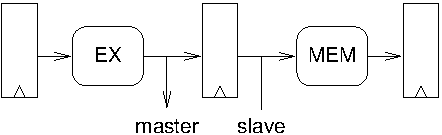
\includegraphics[scale=.8]{fig/ocppipe}
  \caption{Localization of OCP signals in the pipeline}
  \label{fig:ocppipe}
\end{figure}

Figure~\ref{fig:ocppipe} shows the OCP signals in the Patmos
pipeline. The master signals are generated in the execute stage, and
the slave signals are captured in the memory stage.\footnote{For
  clarity, the handling of both parts is implemented in the file
  \code{Memory.scala}.}

\begin{figure}
  \centering
  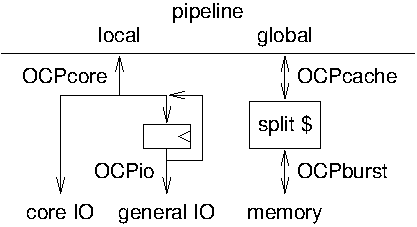
\includegraphics[scale=.8]{fig/ocplevels}
  \caption{OCP levels in Patmos}
  \label{fig:ocplevels}
\end{figure}

The different variants of the OCP protocol in the scope of the Patmos
processor are shown in Figure~\ref{fig:ocplevels}.

\subsubsection{\code{OCPcore}}

The variant of OCP generated by the pipeline for the local address
space. The respective signals are shown in
Table~\ref{tab:coresignals}. \code{OCPcore} is tailored to accesses to
on-chip memories, which on FPGAs necessarily include an internal
register. To enable sub-word transfers of data, the signal
\code{MByteEn} is used. The following assumptions apply:
\begin{itemize}
\item Only reads and non-posted writes are supported. This entails
  that every command must be followed by a response.
\item No \code{SCmdAccept} or \code{MRespAccept}, flow control is done
  solely via \code{SResp}.
\item Slaves may generate responses earliest in the cycle after a
  command.
\item The master may issue commands in the same cycle as the slave
  sends its response, i.e., basic support for pipelining is required.
\item \code{MByteEn} is assumed to be properly aligned
  (\code{force\_aligned=1}). The signal can be ignored for read
  accesses without side-effects.
\end{itemize}

\begin{table}
  \centering
  \caption{\code{OCPcore} signals}
  \label{tab:coresignals}
  \begin{tabular}{ll}
    \toprule
    Signal & Description \\
    \midrule
    \code{MCmd} & Command \\
    \code{MAddr} & Address, byte-based, lowest two bits always 0 \\
    \code{MData} & Data for writes, 32 bits \\
    \code{MByteEn} & Byte enables for sub-word accesses, 4 bits \\
    \cmidrule{1-2}
    \code{SResp} & Response \\
    \code{SData} & Data for reads, 32 bits \\
    \bottomrule
  \end{tabular}
\end{table}

\subsubsection{\code{OCPio}}

The \code{OCPio} level is derived from the \code{OCPcore} level by
inserting a register in the master signals. It is slightly more
flexible than \code{OCPcore} and appropriate for I/O devices that do
not (or cannot) follow the semantics of \code{OCPcore}. Registering
the master signals changes the protocol as follows:
\begin{itemize}
\item Slaves may generate responses in the same cycle as they
  receive a command.
\item Commands are issued earliest in the cycle after a response (no
  pipelining).
\item \code{SCmdAccept} is supported. It is sufficient to register the
  master signals only if the currently registered command is
  \code{IDLE} or \code{SCmdAccept} is high.
\item In order to have symmetric handshaking for commands and
  responses and to facilitate clock-domain crossing, \code{OCPio} also
  includes a signal \code{MRespAccept}. An \code{OCPio} port that is
  derived directly from the pipeline's \code{OCPcore} port always
  accepts responses.
\end{itemize}

\subsubsection{\code{OCPcache}}

This OCP variant is generated for the global address space and is used
for communication between the pipeline and the caches. It is the same
as \code{OCPcore}, but includes an additional signal \code{MAddrSpace}
to specify the cache that should serve the access.

\subsubsection{\code{OCPburst}}

The caches access the external memory through bursts only;
Table~\ref{tab:burstsignals} shows the signals of the \code{OCPburst}
interface. The tie-off value for \code{MBurstLength} is 4, and
\code{MBurstSingleReq} is tied off to 1. This means that the master
supplies four data words for each write command, and the slave returns
four words for each read command. All other burst-related signals are
tied off to their default values. This entails that the only sequence
for burst addresses is \code{INCR}. Bursts always stat at an address
that is aligned to the burst size
(\code{burst\_aligned=1}). Furthermore, \code{reqdata\_together} is
set to 1, i.e., write commands and the respective first word are
issued together. Instead of the signal \code{MByteEn}, \code{OCPburst}
uses the signal \code{MDataByteEn}. This implies that partial write
transfers are fully supported, but partial read commands are
unsupported.

We assume that the master provides data for burst accesses in
consecutive cycles and that slaves can accept all burst data words
once they accept the first word. To enable handshaking for the
acceptance of the first data word, the \code{OCPburst} variant
includes the signals \code{MDataValid} and \code{SDataAccept}. As
\code{reqdata\_together} is set to 1, delaying the acceptance of data
also delays the acceptance of write commands. In order to do the same
for read commands, \code{OCPburst} also includes the signal
\code{SCmdAccept}. The signals \code{SCmdAccept} and
\code{SDataAccept} can be generated by the same logic. For the
acceptance of write commands they must be identical, otherwise at
least one of the signals can have an undefined value. We assume that
slaves return burst read data in consecutive cycles

The first response to a read command may be given in the cycle after
the command. The response to a write command may be given earliest in
the cycle after the last data word was sent. Commands may be issued
earliest in the cycle after the last response from an earlier command
is received.

\begin{table}
  \centering
  \caption{\code{OCPburst} signals}
  \label{tab:burstsignals}
  \begin{tabular}{ll}
    \toprule
    Signal & Description \\
    \midrule
    \code{MCmd} & Command \\
    \code{MAddr} & Address, byte-based, lowest two bits always 0 \\
    \code{MData} & Data for writes, 32 bits \\
    \code{MDataByteEn} & Byte enables for sub-word writes, 4 bits \\
    \code{MDataValid} & Signal that data is valid, 1 bit \\
    \cmidrule{1-2}
    \code{SResp} & Response \\
    \code{SData} & Data for reads, 32 bits \\
    \code{SCmdAccept} & Signal that command is accepted, 1 bit \\
    \code{SDataAccept} & Signal that data is accepted, 1 bit \\
    \bottomrule
  \end{tabular}
\end{table}

\subsection{Remarks}

\code{SCmdAccept} is valid only while a command is unequal to
\code{IDLE}. Consequently, \code{SCmdAccept} must be properly
multiplexed to support multiple slaves. For handshaking via
\code{SResp}, it is sufficient to combine the responses of different
slaves with OR.

\wolf{With \code{writeresp\_enable} we could also require a response
  for ``normal'' writes.}

\wolf{\code{OCPburst} currently allows neither pipelining nor
  same-cycle responses. If we want to, we can make it more like
  \code{OCPcore} or \code{OCPio}.}

\wolf{I am pretty sure that we need to include \code{MDataValid} when
  using single request bursts. Please check if you understand the spec
  the same way.}

Note 4: 
Bursts are restricted to exactly four words (D1, D2, D3 and D4), or some other constant which is a power of 2.  The address must be aligned. Burst data must be provided in four consecutive cycles. SResp is active during these cycles. For a burst write the master may have to provide D1 for two or more cycles if SResp is not active in the first cycle of the transaction.

\wolf{\code{SResp} is \emph{not} active during write bursts according
  to the OCP spec. If necessary, handshaking for write bursts is done
  via \code{SCmdAccept} and/or \code{SDataAccept}.}

\todo{The legal status of using a subset of OCP in an open-source
project needs to be checked. The Patmos document shall be
self contained and no membership to OCP necessary to use
Patmos.}

\clearpage
\subsection{Timing Diagrams}

\subsubsection{\code{OCPcore}}

Figure~\ref{fig:timing_core} shows a sequence read/write/read in
\code{OCPcore}, where the slave delays the response to the write by
one cycle.

\begin{figure}
\centering
\includegraphics{fig/timing_core}
\caption{Timing diagram for \code{OCPcore}}
\label{fig:timing_core}
\end{figure}

\begin{enumerate}[A:]
\item The master issues a read by setting \code{MCmd} to \code{RD},
  \code{MAddr} to \code{A$_1$} and \code{MByteEn} to \code{E$_1$}.
\item The slave responds to the read issued in cycle A by setting
  \code{SResp} to \code{DVA} and returning the appropriate data. The
  master can issue the next command in the same cycle as it receives
  the response and issues a non-posted write command \code{WRNP}. The
  master provides the byte enable value \code{E$_2$} along with the
  data \code{D$_2$} to specify which bytes should be actually written.
\item The slave does not respond immediately and the master is
  stalled. \code{MCmd} must be \code{IDLE} while the master is
  stalled.
\item The slave responds to the write issued in cycle B. The master
  issues a read in the same cycle.
\item The slave responds to the read issued in cycle D.
\end{enumerate}

\clearpage
\subsubsection{\code{OCPio}}

Figure~\ref{fig:timing_io} shows a sequence read/write/read in
\code{OCPio}, where the slave does not accept the write immediately
and delays the response to the write by one cycle.

\begin{figure}
\centering
\includegraphics{fig/timing_io}
\caption{Timing diagram for \code{OCPio}}
\label{fig:timing_io}
\end{figure}

\begin{enumerate}[A:]
\item The master issues a read by setting \code{MCmd} to
  \code{RD}. The slave accepts the command by setting
  \code{SCmdAccept} to high and responds immediately by setting
  \code{SResp} to \code{DVA} and returning the appropriate data.
\item The master issues a non-posted write command \code{WRNP} with
  data \code{D$_2$} and byte enables \code{E$_2$}. The slave
  signals that it does not accept the command by setting
  \code{SCmdAccept} to low.
\item As the slave did not accept the command in cycle B, the master
  still issues the command. The slave accepts the command by setting
  \code{SCmdAccept} to high.
\item The slave responds to the write it accepted in cycle C. Note
  that a) the master is not allowed to issue a new command immediately
  and b) \code{SCmdAccept} may take any value, because \code{MCmd} is
  \code{IDLE}.
\item The master issues a read to which the slave responds immediately.
\end{enumerate}

\clearpage
\subsubsection{\code{OCPburst}}

Figure~\ref{fig:timing_burst} shows a read followed by a write in
\code{OCPburst}, were the slave does not accept the first data word
immediately.

\begin{figure}
\centering
\includegraphics{fig/timing_burst}
\caption{Timing diagram for \code{OCPburst}}
\label{fig:timing_burst}
\end{figure}

\begin{enumerate}[A:]
\item The master issues a read command by setting \code{MCmd} to
  \code{RD}. The slave accepts by asserting \code{SCmdAccept}.
\item The slave provides the first response \code{DVA$_{1.0}$}, with
  data from address \code{A$_1$}.
\item The slave provides the second response \code{DVA$_{1.1}$}, with
  data from address \code{A$_1$+4}.
\item The slave provides the third response \code{DVA$_{1.2}$}, with
  data from address \code{A$_1$+8}.
\item The slave provides the fourth and last response
  \code{DVA$_{1.3}$}, with data from address \code{A$_1$+12}.
\item The master issues a write command by setting \code{MCmd} to
  \code{WRNP} and provides the first data word \code{D$_{2.0}$} width
  byte enables \code{E$_{2.0}$} It signals that the data is valid by
  asserting \code{MDataValid}. The slave signals that it cannot accept
  the data by setting \code{SDataAccept} to low.
\item As the slave did not accept the data in cycle F, the master
  keeps issuing the command and providing the data word
  \code{D$_{2.0}$}. The slave now accepts the data by setting
  \code{SDataAccept} to high.
\item The master provides the second data word, \code{D$_{2.1}$} with
  byte enables \code{E$_{2.1}$}.
\item The master provides the third data word, \code{D$_{2.2}$} with
  byte enables \code{E$_{2.2}$}.
\item The master provides the fourth and last data word,
  \code{D$_{2.3}$} with byte enables \code{E$_{2.3}$}.
\item The slave responds to the write burst by setting \code{SResp} to
  \code{DVA}.
\end{enumerate}

% % % % % % % % % % % % % % % % % % % % % % % % % % % % % % % % % % % % % % % %
\chapter{Implementation}

\martin{This sections shall describe implementation details,
decisions, and options.}

After a first implementation of Patmos in VHDL we did a cleanup and
rewrite in a the hardware description language Chisel~\cite{chisel:dac2012}.
The following notes on the implementation of Patmos and implementation
decisions is based on first design discussions within the VHDL version
and concrete implementation experiments with Chisel. All size and frequency
numbers are from the Chisel implementation. A comparison between VHDL
and Chisel would be of great interest.

LoC, excluding the copyright header at 6.4.2013:
Chisel: 996
VHDL: 3020

\section{Component Organization and Pipeline Structure}

The architecture of Patmos is structured around five components, each
representing one pipeline stage. Each component contains the \emph{left}
pipeline register. E.g., the output of the \code{DEC} stage (decode signals,
the two register values, and the immediate field) is combinatorial from
the decode stage and registered in the \code{EX} stage. The motivation of
this organization is that input registers of on-chip memory elements (e.g., instruction
memory, register file, and data memory) are part of the pipeline register.
They need to be fed unconditionally from the unregistered output of
the former stage.

Each stage has exactly one pipeline register, which is placed at the begin
of the component. The pipeline registers use an enable for stalling.
Register that have no enable (input registers of on-chip memories) need
a \emph{shadow} register and a multiplexer for stalls.

The interface from the EX stage to the MEM stage might use one
field for ALU results and the store data or individual fields. Individual
fields might reduce the pressure on the ALU multiplexers.
\martin{Update to the current implementation -- check for difference.}


\section{Register File}

There are two options to implement the register file (RF) in an FPGA: (1) use
two on-chip memories to provide two read ports and one write port, or (2)
use dedicated registers and larger multiplexer structures for the read
ports. Usually one aims to use on-chip memory for the RF. However,
in a design constraint largely by the available amount of on-chip memory,
a RF built out of registers might be preferable.

For a dual issue pipeline we need 4 read ports and 2 write ports into the RF.
We explored double clocking of a on-chip based RF in~\cite{patmos:ppes2011}.
It is feasible, the resulting maximum frequency fits for the ALU path, but feels
a little bit brittle. A RF from registers might give a more robust design for the
two write ports. Furthermore, Chisel does not provide the possibility to use
more than one clock.

The ideal solution would be to make it configurable if on-chip memory or
LCs are used. The issue width should also be configurable.




\section{Resource and Fmax Numbers}

State 13.3.2013 with Chisel and DE2-70: A shared field (for EX to MEM?) results 3435 LCs
and 81.7 MHz, two fields in 3499 LCs and 81.8 MHz. Looks like not a big deal,
but just 64 more LCs. Where does this cost come from? A very inefficient
enable on the pipeline register (MUX instead of an enable signal?).

\martin{Update with reduced ALU muxes and also with additional second
ALU pipeline (forwarding). Is dual issue configurable?}

\section{ALU Discussion}

The large multiplexers and the forwarding limit the maximum frequency.
We have already removed the expensive rotate instructions. Maybe more
can go (e.g. \code{abs}).

Current version (4.4.2013) with all ALU operations and test case ALU.s
for the DE2-70 is: 3415 LCs, 85.44 MHz. Dropping \code{rsub} and all unary
ALU operations: 3173 LCs, 91.91 MHz.

\section{Building Patmos}

The whole build process of Patmos,%
\footnote{Get the source from GitHub with: \code{git clone git@github.com:t-crest/patmos}}
applications in assembler
and in C, configuration of the FPGA, and downloading an application
is \code{Makefile} based.

The complete design flow (including the LLVM
based C compiler) can execute in a Linux machine. The flow without
the C compiler should be able to execute in a Windows/Cygwin environment.
Under Mac OS X all tools, except Quartus, are working (ModelSim under
wine). For FPGA synthesis and configuration Windows XP within a VMWare
virtual machine is a possible solution.

On a Linux box with the installed LLVM compiler in your PATH,%
\footnote{Installation and build is a simple two step approach:
\code{git clone git@github.com:t-crest/patmos-misc.git misc}
and build with:
\code{./misc/build.sh}}
the complete build processes is kicked of by:

% make BOOTAPP=bootable-bootloader APP=helloworld tools synth comp config download
\begin{verbatim}
make BOOTAPP=bootable-bootloader APP=helloworld \
   tools comp gen synth config download
\end{verbatim}

Here a list of the most important make targets:


\begin{description}
\item[tools] build of all tools, including the Patmos software simulator
\item[asm] assemble source (from folder \code{asm})
\item[emulator] build the Chisel based C++ emulator
\item[csim] execute the Patmos emulator 
\item[comp] compile a C program as loadable ELF binary
\item[bootcomp] compile a C program as a bootable image
\item[gen] generate the Verilog code
\item[synth] synthesize for an FPGA
\end{description}


\todo{Test and describe the ELF download flow.}

The \code{Makefile} use following variables to configure the build process:
\code{BOOTAPP} is an application that ends in the on-chip ROM. This may
be an assembler program or a simple C program that does not need any
initialized data; most prominent the boot loader for ELF binaries.
A C program that shall be compiled as ROM target needs to be prefixed
with \code{bootable-}.
\code{APP} is a C program resulting in an ELF binary that can be either
loaded by the emulator or the boot loader when executing in an FPGA.
% TODO: test and talk about patsim. Having a complete ELF in the FPGA
% without the boot loader would be nice as well.

Here an example of the individual steps to build the blinking LED C
hello world (on a different FPGA board):
\begin{verbatim}
make tools
make BOOTAPP=bootable-echo bootcomp gen
make BOOTAPP=bootable-echo QPROJ=bemicro synth
make QPROJ=bemicro BLASTER_TYPE=Arrow-USB-Blaster config
\end{verbatim}

This split of the make commands is for demonstration. It is
possible to merge all steps into a single make (on Linux
systems) or two steps when using a two operating
systems (for compilation and synthesis).

\chapter{Application Binary Interface}
\label{sec:abi}

\section{Data Representation}

Data words in memories are stored using the big-endian data representation, this
also includes the instruction representation.

\section{Register Usage Conventions}

The register usage conventions for the general purpose registers are as follows:
\begin{itemize}
  \item \texttt{r0} is defined to be zero at all times.
  \item \texttt{r1} and \texttt{r2} are used to pass the return value on
        function calls.
  \item \texttt{r3} through \texttt{r8} are used to pass arguments on function
        calls.
  \item \texttt{r27} is used as temp register.
  \item \texttt{r28} is defined as the frame pointer and \texttt{r29} is defined as the stack
        pointer for the \emph{shadow} stack in global memory. The use of a frame
        pointer is optional, the register can freely be used otherwise. 
	\texttt{r29} is guaranteed to always hold the current stack pointer and is not used 
	otherwise by the compiler.
  \item \texttt{r30} and \texttt{r31} are defined as the return function base
        and the return function offset.
        Usually, they are passed as operands to the \texttt{ret} instruction.
  \item \texttt{r1} through \texttt{r19} are caller-saved \emph{scratch}
        registers.
  \item \texttt{r20} through \texttt{r31} are callee-saved \emph{saved}
        registers.
\end{itemize}

The usage conventions of the predicate registers are as follows:
\begin{itemize}
  \item all predicate registers are callee-saved \emph{saved} registers.
\end{itemize}

\daniel{I have no educated opinion whether caller- or callee-saved.}
\fb{This is rather easy to change in the compiler, and should be evaluated
accordingly.}

\daniel{
What I'd like to have for single-path code is a guard predicate parameter for the called function, e.g., always passed in p1.
}
\fb{What would the guard predicate be good for? If need be we could define a
separate calling convention for single-path-programming programs; in order to
keep the conventions for the other programs sane.}

\stefan{We would gain in most cases by making predicates caller-saved, since predicates are usually not 
used across function calls, this saves up to 6 instructions per call. 
Predicate live ranges over calls only happen with single-path and if-conversion. However, having only caller-saved predicates
makes if-conversion of calls too costly (and too complex). A nicer solution would be to have p1-p4 caller-saved and
p5-p7 callee saved. I got this to work (do not alias s0 with p1-p7 in RegInfo.td, mark s0 and p5-p7 as callee saved 
in RegInfo.cpp, and in processBeforeCalleeSavedScan set s0 as used when any of p5-p7 is used), but this would require the
if-converter to use callee-saved predicates when converting calls, i.e., to change the predicate of the condition.
Sounds easy, but is actually far from trivial to hack into the if-converter, and only works if the if-converter runs before the
prologue-inserter, so we stay with callee saved registers for now and live with the costs of spilling s0 at nearly every call.}


The usage conventions of the special registers are as follows:
\begin{itemize}
  \item The stack cache control registers \texttt{ss} and \texttt{st} are callee-saved
        \emph{saved} register.
  \item \texttt{s0}, representing the predicate registers, is a callee-saved \emph{saved} register.
  \item All other special registers are caller-saved scratch registers and should not be used
        across function calls.
\end{itemize}

\section{Function Calls}
\label{sec:function_calls}

Function calls have to be executed using the \texttt{call}
instruction that automatically prefetches the target function to the method
cache and stores the return information to the general-purpose register \texttt{r31}.
At a function call, the callers base address has to be in \texttt{r30}.
The callee is responsible to store/restore the callers function base and pass it as first
operand to the return instruction. 
The \texttt{call} and \texttt{brcf} instructions neither use nor modify \texttt{r30}, the
return function base is only used by \texttt{ret}.

The register usage conventions of the previous section indicate which registers
are preserved across function calls.

The first $6$ arguments of integral data type are passed in registers, where
64-bit integer and floating point types occupy two registers. All other
arguments are passed on the \emph{shadow} stack via the global memory.

\fb{We could pass arguments via the stack cache, however, this would work only
for functions with a fixed number of arguments. The calling convention for
variadic function would then differ from the standard conventions. We should
probably also introduce a size limit on how many arguments should be passed via
the stack cache. Thus, for a first shot I decided to keep the conventions
simple.}
\martin{I would like to see arguments passed via the stack cache. No
reason to go via main memory (when the number is fixed.}

\martin{BTW: an on-chip stack, with single cycle access, is not so different from
a large register file. Maybe using a sliding window to keep the number of
addressing bits down. Shall we merge the stack cache with the register file?
Are we than redoing a stack (Java) processor?}

When the return function base \texttt{r30} and the return offset \texttt{r31}
needs to be saved to the stack, they have to be saved as the first elements
of the function's stack frame, i.e., right after the stack frame of the
calling function. Note that in contrast to \texttt{br} and \texttt{brcf} the 
return offset refers to the next instruction after the \emph{delay slot} of the 
corresponding \texttt{call} and can be implementation dependent (cf.\ the description
of the \texttt{call} and \texttt{ret} instructions).

\section{Sub-Functions} 
A function can be split into several sub-functions. The program is only allowed to use
\texttt{br} to jump within the same sub-function. To enter a different sub-function,
\texttt{brcf} must be used. It can only be used to jump to the first instruction of a 
sub-function.

In contrast to \texttt{call}, \texttt{brcf} does not provide link information.
Executing \texttt{ret} in a sub-function will therefore return to the last \texttt{call}, not to the last \texttt{brcf}.
Function offsets however are relative to the \emph{sub-function} base, not to the surrounding function. 
The function base register \texttt{r30} must therefore be set to the base address
of the current \emph{sub-function} for calls inside sub-functions.

A sub-function must be aligned and must be prefixed with a word containing the size of the sub-function,
like for a regular function. If a function is split into sub-functions, the first sub-function
must also be prefixed with the size of the first sub-function, not with the size of the whole function.

There are no calling conventions for jumps between sub-functions, for the compiler 
this behaves just like a regular jump, except that the base register \texttt{r30} must
be updated if the sub-function contains calls.


% TODO: examples

\stefan{We need to define how the call and local branch with cache fill get the size of the code to load. A word
containing the size at the target address, or prior to the target address? (including or excluding the size word?)}

\jack{I'd store the code size at the target address and have the
method itself start at an offset +4 or +8 from that place. I also
suggest storing the stack size here too. Could fit into the same
32-bit word (since I'd guess the local memory size limits us to
$<64$k code and $<64$k stack in a single method anyway).}

\martin{Agree for plain C code where there is no data structure
further describing a function. In the JOP JVM I have the luxury
to have those sizes as part of the virtual method dispatch table.
One indirection is there needed anyway, so why not having those
data there.}

\section{Stack Layout}

All stack data in the global memory, either managed by the stack cache or using
a frame/stack pointer, grows from top-to-bottom. The use of a frame pointer is
optional.

Unwinding of the call stack is done on the stack-cache managed stack frame,
following the conventions declared in the previous subsection on function calls.

\section{Interrupts and Context Switching}

Interrupt handlers may use the shadow stack pointer \texttt{r29} to spill registers
to the shadow stack. Interrupts must ensure that all special registers that might be in use 
when the interrupt occurs are saved and restored.

Here is a simple example of storing and restoring the context for context switching.
\begin{verbatim}
sub $r29 = $r29, 40
sws [$r29 + 0] = $r31
sws [$r29 + 1] = $r30
sws [$r29 + 2] = $r22  // free some registers
sws [$r29 + 3] = $r23  
mfs $r22 = $s2  // by now any mul should be finished
mfs $r23 = $s3
sws [$r29 + 4] = $r22
sws [$r29 + 5] = $r23
mfs $r22 = $r5  // read out cache pointers, spill
mfs $r23 = $s6
sub $r22 = $r23, $r22
sspill $r22   // spill the memory, s5 == s6 now
sws [$r29 + 6] = $r22  // store the stack pointer
sws [$r29 + 7] = $r23  // store stack size
... 
// TODO store return base and offset

// restore
lws $r23 = [$r29 + 7]
lws $r22 = [$r29 + 6]
mts $s5 = $r22   // restore the stack
mts $s6 = $r22
sens $r23
lws $r23 = [$r29 + 5]
lws $r22 = [$r29 + 4]
mts $s2 = $r22
mts $s3 = $r23
....
\end{verbatim}

\stefan{We need to define how to register interrupts, how to return from interrupts (where do we get
the return-base and return-offset from,..). Interrupt handlers in C are currently not supported, 
the compiler does not restore all the special registers for normal functions.}


% % % % % % % % % % % % % % % % % % % % % % % % % % % % % % % % % % % % % % % %
\chapter{Potential Extensions}

\section{Exceptions: Interrupts, Faults and Traps}
\label{sec:exc}

\wolf{These is a first attempt to specify how we could/should
  implement asynchronous transfer of control.}

In the following, we use \emph{exception} to denote any kind of
``abnormal'' transfer of control. \emph{Interrupts} are generated
outside of the pipeline by I/O devices. \emph{Faults} are triggered by
the pipeline for instructions that cannot be executed as expected
(accesses to unmapped memory, undecodable instructions,
etc.). \emph{Traps} are willfully generated exceptions, and are used
to invoke operating system functions, which might require elevated
privileges (see Section~\ref{sec:supervisor}).

An \emph{exception unit} that is mapped to the I/O space is
responsible for managing exceptions. It includes the device registers
shown in Table~\ref{tab:excioregs}. The general principle of operation
is that the exception unit requests the execution of an exception from
the pipeline, and the pipeline returns an acknowledges when it starts
the execution of the respective exception handler.

\begin{table}
  \centering
  \begin{tabular}{llp{.6\textwidth}}
    \toprule
    Address             & Name             & Description \\

    \texttt{0xf?????00} & \texttt{status} & Interrupt-enable flag,
    possibly privilege bits. Left-shifted on start of exception
    handler, right-shifted when returning. \\

    \texttt{0xf?????04} & \texttt{mask} & Mask of enabled interrupts \\

    \texttt{0xf?????08} & \texttt{pend} & Pending flags for interrupts \\

    \texttt{0xf?????0c} & \texttt{source} & Number of exception that
    is about to be served \\
    
    \cmidrule{1-3}

    \texttt{0xf?????20} & \texttt{vec<0>} & Address of exception handler 0 \\
    \texttt{0xf?????24} & \texttt{vec<7>} & Address of exception handler 1 \\
    \ldots & \ldots & \ldots \\

    \bottomrule
  \end{tabular}
  \caption{Exception unit device registers}
  \label{tab:excioregs}
\end{table}

Exceptions are injected into the pipeline in the decode stage. The
decode stage was chosen to do this because
\begin{enumerate}
\item Interrupts must not be triggered inside branch delay slots. The
  decode stage ``knows'' which instructions are executed and can
  easily keep track of branch delay slots.
\item Mechanisms for calls that are located in the execute stage can
  be shared with exception handling.
\end{enumerate}

All exceptions that have their origin in the pipeline (faults and
traps) are handled through signals from the memory stage to the
exception unit. The memory stage is responsible for aborting the
execution of any unfinished instructions (flushing the pipeline). The
exception unit is responsible for demanding the injection of the
correct exception from the decode stage.

To be able to serve exceptions generated by the pipeline when an
interrupt already has been injected, the acknowledgment from the
pipeline to the exception unit is generated in the memory unit. Only
at this point it is clear if the interrupt will be served or if the
injected instruction has been flushed from the pipeline.

The memory unit furthermore includes a signal to notify the exception
unit of returns from exception handlers.

\begin{table}
  \centering
  \begin{tabular}{llp{.6\textwidth}}
    \toprule
    Name & Stage & Description \\
    \midrule
    \texttt{intr}    & to Decode & Request injection of interrupt, must be ignored in delay slot \\
    \texttt{exc}     & to Decode & Request injection of other exception, cannot be ignored \\
    \texttt{excaddr} & to Decode & Address of exception handler to be executed \\
    \texttt{exccall} & from Memory & Acknowledge execution of exception handler \\
    \texttt{excret}  & from Memory & Notify exception unit of return from exception handler \\
    \bottomrule
  \end{tabular}
  \caption{Exception unit signals to pipeline}
\end{table}

\subsection{Changes to ISA}

In order to support exceptions, it is necessary that the base address
of the current function is available \emph{at any time}. Otherwise, it
could not be guaranteed that an interrupt handler is able to return to
the correct function. Consequently, the \texttt{call} and
\texttt{brcf} functions must store the base address in some hardware
register. This makes the return-base information in register
\texttt{r30} redundant and it could be replaced by an appropriate
special return base register \texttt{sb} with minimal effort.

The return information for exceptions must be stored in registers that
are not used otherwise. Two special registers \texttt{sxb} and
\texttt{sxo} provide the return base and return offset for exceptions.

Depending of on the exact implementation, delayed loads might require
another special register to save the contents of the special register
\texttt{sm} upon exceptions.

For traps, we introduce an instruction \texttt{trap <n>}, which
triggers exception number $n$. In order to assimilate the handling of
faults and traps, the \texttt{trap} instruction causes the memory unit
to signal an exception to the exception unit, which then requests the
injection of an exception from the decode unit. Consequently, traps do
not have a delay slot despite altering the control flow.

To signal the return from an exception handler, we introduce an
instruction \texttt{xret}, which causes the exception unit to update
the status word appropriately.

\subsection{Resuming Execution}

Resuming execution after an interrupt is straight-forward. The
interrupt handler simply returns to the bundle that was replaced by
the injected interrupt instruction.

Resuming after a fault requires a bit more thought. In principle,
execution could resume after the instruction that caused the fault, or
retry execution of the instruction. Retrying execution would be
suitable for faults like page faults, but would be inappropriate for
faults like an accesses to an address that is not mapped to any memory
or I/O device or undecodable instructions.

The issue is further complicated by instructions in the other slot of
a bundle, whose effects must be made visible when resuming
execution. Consider the scenario that the instruction in the first
slot is faulty. The instruction in the second slot may use a register
that is modified by the instruction in the first slot. Emulating the
first instruction and simply resuming with the second instruction is
therefore not correct. If the instruction in the first slot uses a
register that is modified be the instruction in the second slot,
letting the instruction in the second slot continue to the write back
stage before executing the exception handle would incorrect.

As a consequence, resuming execution must either fix the cause of the
fault and reexecute the whole bundle again, or emulate the effects of
the whole bundle (including the triggering of further faults) and
continue execution after the bundle. Due to the complexity of the
second option, we consider faults where the respective instruction
cannot be reexecuted \emph{fatal}, and advise developers to terminate
execution instead of trying to resume. For faults, the return address
points to the bundle that triggered the fault.

Resuming after a trap in principle has to take into account the same
considerations as faults. However, the content of the bundle is under
the control of the compiler. We require that a trap instruction is the
only instruction in a bundle. The return address for traps points to
the bundle after the one that contains the trap instruction.

\subsection{Older Comments}

\emph{also delayed exceptions for speculative execution}

\wolf{I don't think delayed exceptions are a good idea, given that
  doing a clean restart after the exception would be even messier than
  it is now.}

\begin{itemize}
  \item Enable/disable interrupts
  \item Return from interrupt
  \item Interrupt vector tables or something along these lines
  \item What happens to ongoing memory accesses through the method cache, stack
        cache or decoupled loads?
\end{itemize}

\martin{We need to be careful what happens in an interrupt in the
branch delay slots -- Marco has fought this in the simulator, right?
Also an issue for 64-bit atomic read of time register and some
care to be taken for the multiply.}

\clearpage
\subsection{Timing Diagrams}

\subsubsection{Interrupt}

Figure~\ref{fig:timing_intr} shows the triggering of an interrupt.

\begin{figure}[t!]
  \centering
  \includegraphics[scale=.95]{fig/intr}
  \caption{Interrupt, delayed by branch delay slot}
  \label{fig:timing_intr}
\end{figure}

\begin{enumerate}[A)]
\item The decode stage decodes a branch instruction \texttt{BR}.
\item As the previous instruction was a branch and the current bundle
  is part of a branch delay slot, the signal \texttt{dec.indly} is
  high.
\item The exception unit requests an interrupt by asserting
  \texttt{xu.intr}. As \texttt{dec.indly} is still high, the request
  is ignored.
\item The signal \texttt{xu.intr} is still asserted, but the current
  instruction is not part of a branch-delay slot, so the decode stage
  generates an interrupt instruction \texttt{INTR}.
\item The interrupt has not been acknowledged, so signal
  \texttt{xu.intr} is still asserted and the decode stage generates
  another interrupt instruction. The previous interrupt instruction
  reaches the execute stage.
\item The interrupt instruction reaches the memory stage, which
  acknowledges the interrupt and flushes the pipeline.
\item The fetch stage fetches the first instruction of the interrupt
  handler, \texttt{OP$_9$}.
\item The first instruction of the interrupt handler reaches the
  decode stage.
\item The first instruction of the interrupt handler reaches the
  execute stage.
\item The first instruction of the interrupt handler reaches the
  memory stage.
\end{enumerate}

\subsubsection{Fault}

Figure~\ref{fig:timing_exc} shows the triggering of a fault while an interrupt is requested.

\begin{figure}
  \centering
  \includegraphics{fig/exc}
  \caption{Fault while interrupt is requested}
  \label{fig:timing_exc}
\end{figure}

\begin{enumerate}[A)]
\item The exception unit requests an interrupt and the decode stage
  generates an instruction \texttt{INTR}.
\item While the interrupt instruction is in the execute stage,
  instruction \texttt{OP$_2$} in the memory stage causes a fault. The
  memory stage signals this to the exception unit and flushes the
  pipeline.
\item The exception unit now requests a (non-interrupt) exception and
  an interrupt. As (non-interrupt) exceptions take precedence, the
  decode stage generates an instruction \texttt{EXC}.
\item Instruction \texttt{EXC} reaches the execute stage.
\item Instruction \texttt{EXC} reaches the memory stage, which
  acknowledges the exception and flushes the pipeline again.
\item The fetch stage fetches the first instruction of the exception
  handler, \texttt{OP$_8$}.
\item The first instruction of the exception handler reaches the
  decode stage.
\item The first instruction of the exception handler reaches the
  execute stage.
\item The first instruction of the exception handler reaches the
  memory stage.
\end{enumerate}

\section{Decoupled Loads / Multiply / Wait / Move from Special}

\begin{itemize}
  \item Attaching a ready flag with all special registers.
  \item Specify destination special register with all decoupled operations; the
        operation sets/resets the ready flag accordingly.
  \item Wait operates on ready flags of special registers.
  \item Merged variant of Wait + Move from Special
  \item Wait with 16-bit mask to wait for multiple outstanding results.
\end{itemize}

This would be nice since it would allow to reload all special registers from
memory without going through the general purpose registers. It would be a
unified interface for decoupled operations and give more freedom to handle
parallel decoupled operations (pipelined multiplies, loads). We could apply this
also to the general purpose registers instead of the special registers.

\stefan{I think it makes more sense to use the ready flags with the general purpose registers. Then we can simply replace
all blocking and decoupled loads with special move by one unified load to a general purpose register. This however means
that all operations can potentially stall.}

\stefan{Regarding having additional write ports for the register file: We could still disallow multiple parallel loads by stalling a load
instruction until the last memory op is completed (else we would also need to take some special care of stores if loads and stores can be in progress at the same
time), this would not be any worse than the current ISA (currently we cannot have multiple loads to main memory in parallel). If a load is
ready, I guess we could just stall the pipeline for one cycle to write to the register. Again, this may still be better than the 
current ISA, since we do not need the code space for the additional move from special instruction, but it may cost one stall whereas the
move-from-special could be scheduled in the second slot parallel to some other operation (ok, but then its not so RISC anymore..).}

\section{Bypass load checks data cache}

Let the bypass load use the data cache if the data is cached. If the data is not in the cache, load it from main memory, but do not update
the data cache (in contrast to the normal load). Therefore the compiler could use bypass to load data that will not be used a second time or
that might have a negative impact on the cache analysis, but we still take advantage of the cache if the data is already in the cache.

\stefan{For now the bypass is defined as load always from memory, even if it is in the cache, but there is no real disadvantage to checking the
cache first (except that bypass cannot be used to achieve a perfectly stable timing). But should a bypass update the LRU if it is a cache
hit? (probably not, it should not modify the cache state).

On the other hand, for synchronization we need a bypass that \emph{always} checks main memory. For consistency reasons, we may want to
update the data cache if it contains the accessed address.}

\section{Merged Stack Cache Operations and Function Return}

This might require an additional special-purpose register(?) to track the size
of the last reserve instruction (this register might also be set explicitly).
However, it would might reduce the number of ensure instructions needed.

Another option would be to merge the return and stack free operations. Both
instructions belong to the same function and, due to the simpler semantics of
the free, the combination would be easier to implement.

\stefan{I doubt that merging those functions would actually gain something. It reduces the flexibility for the compiler to perform ensure
only where needed, may limit the possibilities for passing data over the stack cache, and requires additional
code to restore the special registers that are required to track the size of the stack. Only gain I see is when the word in front of the 
method code that stores the size of the method is used to store the stack size as 16bit value, and limit the size of the method to a 16bit
value. Then no additional data needs to be transferred. The stack control instructions would still be required to allow the compiler to
allocate stack e.g. only in certain contexts.}

\martin{If stack operations only happens at function call
and return this merge would make sense. It makes also
very clear that M$ memory access and S$ memory access are coordinated.}

\section{Non-Blocking Stack Control Instructions}

Currently, all stack control operations, except \texttt{sfree}, are blocking. It
might be useful to define non-blocking variants or define them to be
non-blocking in all cases.

It is questionable whether this would actually buy us anything. Most
\texttt{sres} instructions will be followed by a store to the stack cache
(spill of saved registers). It might be more profitable for \texttt{sens}
instructions.

\section{Purge Cache Content}
\begin{itemize}
  \item dynamic code generation, self-modifying code, etc.
  \item help cache analysis?
\end{itemize}

\stefan{Might not gain much: for LRU caches there is no need to purge, we might need to purge the stack cache on context switches anyway,
and for the method cache, purging the cache might also not gain much (depending on the used analysis). I do not think that Self-modifying
should be used in hard real-time code anyway, as it might introduce some slight problems to the WCET analysis ;) }

\section{Freeze Cache Content}

\begin{itemize}
  \item Bypass load can be used to avoid cache updates, but not on per-context basis (we cannot lock the cache and then call any function
  and assume the function does not update the cache. Instead we would need to generate function variants that only use bypass loads).
  \item Method cache freeze? Or should we just use a I-SPM for this if we want instruction cache locking?
\end{itemize}

\section{Unified Memory Access}

\stefan{All our memories (except the stack cache) use a unified address space, but due to the typed loads, references must include both address and
type of the cache. Since the type is encoded in the code, any generated code can only use one type of cache or SPM. 
If we have a function with $m$ arguments and $n$ different caches or ways of accessing
memory, in the worst case we would need $m^n$ copies of that function to handle all cases (increases instruction cache costs!). We also need to expose this to the programmer,
either through having different names for the functions (very ugly and annoying to use, remember that this is transitive, you need to copy
your whole libraries!), or by having a type system on top of the C types, which means implementing some sort of overloading in C and
auto-generating variants of functions.

Note: we need typed loads to tell the processor which cache (not) to use. We also need a shadow stack not only due to typed loads,
but also due to the write-back policy of the stack cache (would make consistency a night-mare if we would allow to access stack-cache
allocated data over the data cache!).
}
\martin{we discussed that issue in The Vienna mini workshop and should continue to discuss it.}

Instead of having typed loads per cache or SPM, maybe have types per ``use-case scenario'', use local memory based on address
\begin{itemize}
\item Type for stack access (guaranteed hit, can be used in both slots)
\item Type for guaranteed hit (any local SPM access, access to data cache must be always hit, else undefined result)
\item Type for unknown data access (access SPM or data cache, or main memory and update data-cache)
\item Type for bypass (access SPM or main memory, do not allocate in data cache)
\item Maybe a type for no-allocate (access SPM, data cache or main memory, but do not allocate data in cache; could be useful to prevent
single loads from thrashing the cache), or use some sort of cache-lock instruction instead (could be useful to prevent a code sequence or function call from
thrashing the cache)
\end{itemize}

\stefan{
The idea behind the typed load is 1.~it makes analysis simpler by having guaranteed hit instructions, 2.~it makes the hardware
simpler and faster (I assume), no need to read the address to determine the local memory to use. 
However, typed loads shift the analysis effort to the compiler, but while the analysis may make over-approximations about the accessed
memory, the compiler must always know the correct memory type, which requires either a precise analysis or help from the programmer by
additional annotations. An analysis can also be context-sensitive, but it is not possible for the compiler to generate ``context-sensitive
typed loads''. A better way for 1.~could be to generate annotations for memory accesses by the compiler instead of putting the
information into the code, which then can be context-sensitive and imprecise and allows for better code reuse, although this (mostly) eliminates the advantages of 2.
Might be interesting to compare those two approaches.
}

\stefan{Note: if we use a DMA controller, we do not need separate memcpy functions depending on the source and destination memory, since the
DMA controller can determine source and target based on the addresses (hopefully).
}

\section{Memory Management Unit}
\begin{itemize}
  \item Simple software managed TLB.
  \item Main idea is to provide protection and separation.
  \item Could be used for memory testing.
  \item No traps. Instead, reset or kill thread?
\end{itemize}

\section{Supervisor Mode}
\label{sec:supervisor}
\begin{itemize}
  \item To restrict reconfiguration of critical components (e.g., TLB, Interrupt
        Tables).
  \item Transfer to supervisor mode, e.g., via \texttt{syscall}.
  \item Might be handy when running multiple threads or an OS.
\end{itemize}

\section{DMA Interface}
\begin{itemize}
  \item Transfers between local and global memory
  \item Through special registers
  \item Alternatively, dedicated instructions \texttt{dmastart} and \texttt{dmalen}
\end{itemize}

\begin{bytefield}{32}
\bitheader{0-31}\\
\bitbox{1}{x} & \bitbox{5}{01010} &
\bitbox{4}{Pred} & \bitbox{5}{Type} & \bitbox{5}{Ra} & \bitbox{5}{Rs} &
\bitbox{7}{} \\
\end{bytefield}

\begin{tabular}{lll}
Type  & Mnemonic & Operation \\ \hline
00001 & dma.sp   & Start memory copy \\
      &          & which contain the word \\
xx001 & st.sc    & Stack cache, no write through to \\
      &          & main memory, never wait \\
xx010 & st.sp    & Scratchpad, no write through to \\
\end{tabular}

\stefan{If the I-SPM and D-SPM has a separate connection to the NoC, we may
also want a separate wait that stalls until the transfer is complete, independent of other memory transfers (load and stores using the data cache).}

\jack{Very useful to have both a blocking and a non-blocking
version of this instruction. The blocking version is probably
more important, though, so if it has to be one or the other,
then blocking should be it.

I-SPM should not really be a concern right now. I'd see this as
a store for permanently-resident code, therefore not requiring DMA.

What does worry me here is the number of DMA routes that might be
possible. I think we need to carefully consider what DMA operations
are really needed. There are three sources/destinations of interest:
stack cache (sc), local memory (lm) and global shared memory (gm),
and they're all effectively in different memory spaces.

I think we want to be able to transfer data from either
lm or sc, to gm. And vice-versa. This gives four DMA routes:
gm~$\rightarrow~$lm, gm~$\rightarrow~$sc, lm~$\rightarrow~$gm,
sc~$\rightarrow~$gm.

I would suggest that there should be a 2-bit field to say which DMA route
should be used and a 1-bit field to say if the operation should block
or not.}

\stefan{The stack cache spill and fill ops are performed by dedicated instructions, so we do not need to support this in the ISA (but it
will probably be handled by the DMA in the background). Do we also handle method cache fill by the DMA (probably yes)? Prefetching into the data cache
(probably not)? 

Accessing main memory over the data cache or with bypass will basically access words in more or less random locations. Stack cache fill and
spill, method cache fill, and DMA transfers from main memory to scratchpad and back perform burst writes. Communication between scratchpads
may be somewhere in between? Maybe we could have two connections to the NoC, or two NoCs, with different package sizes,.. to support the
different transfer scenarios more efficiently. However, the bottleneck will
then be the SDRAM controller.}

\martin{I see also (at least ;-) two NoCs: one for main memory related transfers and one for
message passing communication between SPMs. And those have kind of different DMAs.
The SPM message passing has a real DMA -- I mean one that is programmed by the
CPU like: start from this address and load so many words. The other (caches) memory
transfer is also done by a small state machine - be it cache line fill, method cache several
block fill, or stack cache range fill. However, this bursty transfer is more implicit and
I would not call it DMA.

However, this might just be a naming convention issue. Maybe we are playing
with architectures and naming conventions in a spectrum. E.g. instruction
memory: plain I\$ -- I\$ with prefetch instructions -- method cache -- SPM with
pointer redirect (address translation) -- plain SPM in its own address space.} 

\section{Data scratchpad}

\begin{itemize}
  \item Every core has its D-SPM with its own address range (all in the same address space), a core can write to the D-SPM of another core
  by writing to an address of the SPM of that core.
  \item Maybe have some sort of protection mechanism, to prevent cores from writing to any address in any remote SPM
  \item How do we handle writes to the same address by (remote) dma transfers and local writes (this might prevent local load and stores to
  the SPM from completing in a single cycle)?  \jack{This sounds
    like undefined behavior. The program should avoid doing this.
    But local loads/stores must take priority over remote loads/stores
    to SPM (including locally-initiated DMA transfers) because otherwise
    we will not have single-cycle access to SPM. There must be fixed-priority
    arbitration giving the CPU top priority.}
\end{itemize}

\stefan{The compiler needs to generate typed loads for SPM access. How do we tell the compiler when to use SPM access, without causing too
much pain to the programmer (we would need to annotate all variables, including function arguments and pointers to SPM allocated data). 
Same problem here as with stack cache and second data cache due to typed access: Passing data to a function requires the function to know in which memory the
data is stored. We need specialized functions for
memory types of parameters, in all occurring combinations, this increases code size and method cache misses.}

\martin{I see the D-SPM mainly as buffer for core-to-core message passing.
DMAs transfer data between the NoC and the D-SPM on one memory port
and the CPU accesses it on the other (we are assuming two ports that can
change the direction, which was (is?) not available on all FPGA families).

Part of this D-SPM can also be used just to hold core local data. We don't
need to have an extra one.

Write access to the same address from two sides is simply undefined.
Why shall we provide HW for that? It is a programming error anyway.}

\section{Halt}
\fb{Might not be needed for now. In the simulator we could simply jump to a
label \texttt{exit} or \texttt{halt} or do an explicit syscall to quit the
simulation.}

\section{Floating-Point Instructions}

\section{Prefetching}

\begin{itemize}
  \item For method cache
  \item For local memory
\end{itemize}

\stefan{Prefetching with Method cache with FIFO is tricky, maybe we can use an I-SPM to store code that is executed while we prefetch the
method cache.}

\section{Data Caches}

\begin{itemize}
  \item Add a second (possibly larger), simple (direct mapped,..) data cache, to be used when the pointer address is known at compile time
    (i.e., a load does not destroy the whole cache state in the analysis), for array operations, ..
  \item We would need additional types in the load operation for that cache, but there are only two unused types left. Either use only
    blocking (?) loads and only word and byte (?) access, or replace some lesser used types, or even introduce a new opcode somehow..
\end{itemize}

\stefan{There were some plans about introducing two separate data caches, one direct mapped and a small fully associative (B1.1.6
in the final DoW), with the intention to avoid having loads from unknown addresses destroy the direct mapped cache state in the analysis.
Therefore we might want to reserve some types for loads that use a second data cache (if we do not use write-allocation for store, we do not need to make
this distinction for the store operation).}

\stefan{We also need to define how the store operation performs the data cache updates. I would suggest/prefer to merge the \texttt{gm} and
\texttt{dc} store types, use write-through (to avoid hard-to-analyze write-back costs at some random loads) without write-allocation (to
avoid problems with byte and half-word stores and unnecessary cache conflicts). A store should update all data caches that contain the data.
Then a load immediately after a store to the same address does not need to wait for the store write-through to complete if the load is a cache hit.}

\stefan{Actually, a second data cache with typed loads would be tricky for the compiler. We cannot simply pass a pointer to a constant to a
function that takes any kind of data. if the constant is in a different cache the function does not know this and loads the data also into
the first cache, making the second cache very inefficient.}

\martin{We can overdue it by adding some more data caches: one for
static data (as mentioned before where addresses are known) and one
for constants. The difference is cache coherency, which is not needed
for constants. But are we considering cache coherence?}

\section{Instruction scratchpad}

\begin{itemize}
\item For instruction handlers or other code that should not destroy the method cache
\item Could be used to store code that is executed at a call site (even if the method cache entry of the caller gets replaced)
\item Replacement of code at runtime, statically scheduled or with some sort of software-controlled replacement strategy (maybe this could
be used to prevent threads from destroying the I-cache of real-time tasks)
\item Keep frequently used code on the I-SPM, can be used to do some sort of cache locking (instead of somehow locking the method cache).
\end{itemize}

\jack{I suggest that an I-SPM should be used only to store
permanently resident code. Interrupt handlers, scheduler,
that sort of thing.  Otherwise we need a more complex DMA
controller (more ports) and we need to explain why the I-SPM is
sometimes better than using the method cache. This is a bit tricky
because while dynamic (run-time replacement) I-SPM allocation strategies
do have the advantage of being able to load parts of methods, or pack
multiple methods into a single load, and thus get better performance
in some cases, you can get the same behavior by manipulating the
control flow graph (inlining/exlining/combining methods) and using
a method cache. So it is hard to make that argument in a report.}


\section{Wired-AND/OR for predicates}

Let \texttt{cmp} be some operation that sets a predicate \texttt{Pd} and is predicated by \texttt{Pred}.
Then we could define the following variants:
\begin{verbatim}
cond:   if (Pred)           Pd = <cmp>
and:    if (Pred && !<cmp>) Pd = False
or:     if (Pred &&  <cmp>) Pd = True
uncond: Pd = Pred && <cmp>
\end{verbatim}
Note that we do not need to read \texttt{Pd}, but the last variant uses \texttt{Pred} as input, not as write-enable signal. First variant is
the normal (conditional) execution. The last variant forces \texttt{Pd} to \texttt{false} if \texttt{Pred} is false, thus saving the
initialization of \texttt{Pd} or explicit \texttt{and} with \texttt{Pred} for code like
\begin{verbatim}
if (p1)  p2 = R1 < R2
if (p2)  ...
\end{verbatim}
The other variants can be used to implement stuff like
\begin{verbatim}
if (a != 0 && b < 5) { .. }

p1  = cmpnez r1,    addi r3 = r0 + 5;
p1 &= cmplt r2, r3
\end{verbatim}
To implement \texttt{a != 0 \&\& b > 1} we would need an additional bit that negates either the result of \texttt{<cmp>} or the value that is
assigned to \texttt{Pd} (including the \texttt{true} and \texttt{false} assignments).

Note that if we do not need \texttt{Pred}, we can do \texttt{and} and \texttt{or} simply as
\begin{verbatim}
Pd &= <cmp>  ... if ( Pd)  Pd = <cmp>
Pd |= <cmp>  ... if (!Pd)  Pd = <cmp>
\end{verbatim}
i.e., we use \texttt{Pd} as \texttt{Pred}.


\section{Deadline instruction}

\begin{bytefield}{32}
\bitheader{0-31}\\
\bitbox{1}{x} & \bitbox{5}{01011} &
\bitbox{4}{Pred} &
\bitbox{22}{Counter} \\
\end{bytefield}

Wait until the deadline counter reaches zero, then restart the counter with the given initial value.

\stefan{Do we want this? This is similar to the PRET deadline instruction. We could use this to fix the execution time
of some CFG region, e.g., if we know that in a sequence of load instructions at most one load will be a cache miss, but we do
not know which one, then we can set a deadline to that sequence that allows for one cache miss, and get stable timings for the
program without forcing every memory access that we cannot guarantee to be always-hit to be a cache-miss. We could also use
that instruction to verify the WCET results, by raising an exception if the counter already reached zero when the deadline instruction
is issued. However, we have no exception-handling in our ISA so far..}

\cullmann{For timing analysis, I see no benefit in having the deadline instruction.
Our aiT tool-chain copes well with block with variable durations and can use that to get actually a better WCET bound. (e.g. if for some calling contexts a block is fast, this will be exploited in the analysis)
On the other side, if a deadline instruction is around, we would need to keep track of the current active deadline counter which will increase the complexity of the analysis.
(if I understand it right, that you can at one time start such a deadline and later at an other point wait for it)
}
\stefan{The deadline instruction is basically a tool to make the \emph{measured} execution time more stable. The idea here is to set the
deadline counter based on the WCET analysis, not the other way round (we can set the counter to zero for analysis, so no deadline
instruction will ever wait and the analysis can ignore the instructions, and then use the analysis results to set the counters in the final
code).}
\stefan{Actually, there are only two real use-cases for a deadline instruction: test WCET analysis results (by throwing an exception if
deadline already expired when the instruction is executed, but this requires exception handling in our ISA first!), and making the timing of
\emph{output} produced by the program stable (by waiting on the deadline directly before producing some output; This allows to generate some
periodic signals without having some timer hardware or timer interrupts, i.e., without interrupting the control-flow, thus really bringing
the notion of time into the ISA!).

There is a third use-case: we can fix the execution time of basic-blocks or some code regions. This could be used to make the WCET
of the program more composable by reducing problems with timing anomalies, and to avoid cases where the processor state depends on
the timing of some previous instructions. However, I \emph{strongly} suggest to formally check our ISA and our code generator to be
free of timing anomalies,.., so that we avoid this use-case by design. We want to be able to calculate the WCET for some sub-CFG from the
WCET of the basic-blocks as easily as possible, so that we can keep track of the WCET/WCEP in the compiler when doing code
transformations.}

\chapter{Conclusion}
\label{sec:conclusion}

Patmos is the next cool thing in the dry world of real-time systems.

\bibliographystyle{abbrv}
\bibliography{patbib.bib}

\appendix

\end{document}

\chapter{Archived Discussions}

\begin{itemize}

\item ALU immediate (add, or, and, xor), the function is indicated with \emph{ff}: \\

\begin{bytefield}{32}
\bitheader{0-31}\\
\bitbox{1}{x} & \bitbox{3}{000} & \bitbox{2}{ff} &
\bitbox{4}{Pred} & \bitbox{5}{Rd} & \bitbox{5}{Rs1} &
\bitbox{12}{Constant}\end{bytefield}\\

\begin{tabular}{lll}
ff & Name & Semantics \\ \hline
00 & add & Rd = Rs1 + $\sconst$ \\
01 & or  & Rd = Rs1 \OR $\sconst$ \\
10 & and & Rd = Rs1 \AND $\sconst$ \\
11 & xor & Rd = Rs1 \XOR $\sconst$
\end{tabular}

\stefan{Is Constant sign extended? We have the long immediate ALU instruction anyway, so we do not
need sign extension here, but then we cannot use this short form for subtraction.}
\martin{Yes, it is sign extension.}
\cullmann{Question: for the add, sign extension makes sense, but for the logic stuff, I see no real reason to sign extend, beside that you then only can use 1 bit less of the constant.}
\fb{Might be a good idea to spend some more bits on \texttt{ff} here -- to merge
    the \emph{ALU very short immediate} format introduced by Stefan (except for
    \texttt{rl}). Merge with \texttt{ldi}. \texttt{xor} might not be that
    relevant here, we could replace it with \texttt{sub} and then consider the
    constant to be unsigned.}


\item ALU function: \\

\begin{bytefield}{32}
\bitheader{0-31}\\
\bitbox{1}{x} & \bitbox{5}{00101} &
\bitbox{4}{Pred} & \bitbox{5}{Rd} & \bitbox{5}{Rs1} & \bitbox{5}{Rs2} &
\bitbox{7}{0~\textbar~Func}\end{bytefield}\\

\begin{tabular}{lll}
Function & Name & Semantics \\ \hline
0000000 & add  & Rd = Rs1 + Rs2 \\
0000001 & or   & Rd = Rs1 \OR Rs2 \\
0000010 & and  & Rd = Rs1 \AND Rs2 \\
0000011 & xor  & Rd = Rs1 \XOR Rs2 \\
0000100 & sub  & Rd = Rs1 - Rs2 \\
0000110 & nor  & Rd = \NOT (Rs1 \OR Rs2) \\

0001000 & sl   & Rd = Rs1 \shl Rs2 \\
0001001 & sr   & Rd = Rs1 \shr Rs2 \\
0001010 & sra  & Rd = Rs1 \ashr Rs2 \\
0001011 & rl   & Rd = (Rs1 \shl Rs2) \OR \\
        &      & \phantom{Rd = }(Rs1 \shr (32-Rs2)) \\

0010000 & carr & Rd = ((uint64\_t)Rs1 + \\
        &      & \phantom{Rd = }(uint64\_t)Rs2) \shr 32 \\
0010001 & borr & Rd = ((uint64\_t)Rs1 - \\
        &      & \phantom{Rd = }(uint64\_t)Rs2) \shr 32 \\

??????? & shadd  & Rd = Rs1 + Rs2 \shl 1 \\
??????? & shadd2 & Rd = Rs1 + Rs2 \shl 2 \\
\end{tabular}

\fb{What is the semantic of shifts when \texttt{R2} \textgreater~32 or
    \texttt{R2} \textless~0? I would suggest to consider the lower 5 bits only.}

\stefan{Wolfgang will probably recognize a lot of this.. I shamelessly copied most of the arithmetic
and condition stuff from the Lemberg ISA, so that Martin can copy the implementation and I can copy the compiler ;) }
\martin{Is an ISA under copyright ;-) I'm not sure if I really want all of that, but lets see...}

\stefan{Do we want to have compare instructions that store the result in registers? We could use the same Function code as
for the compare-to-predicate instruction, including compare with immediate value..}
\martin{Compare instructions set a predicate.}

\cullmann{Can't we just allow all ALU functions that take 2 arguments in both ways? e.g. one with R and imm, one with R1 and R2. Would make the ISA for ALU instructions more regular.}


\item Compare (constant could be Rs2 field). It is predicated and has a
destination predicate field: \\

\begin{bytefield}{32}
\bitheader{0-31}\\
\bitbox{1}{x} & \bitbox{5}{01000} &
\bitbox{4}{Pred} & \bitbox{2}{\bitsunused} & \bitbox{3}{Pd} & \bitbox{5}{Rs1} & \bitbox{5}{Rs2} &
\bitbox{7}{Function}\end{bytefield}\\

\begin{tabular}{lll}
Function & Name & Semantics \\ \hline
??????? & cmpz  & Pd = Rs1 ==  0 \\
??????? & cmpnz  & Pd = Rs1 !=  0 \\
0100000 & cmpeq  & Pd = Rs1 ==  Rs2 \\
0100001 & cmpne  & Pd = Rs1 != Rs2 \\
0100010 & cmplt  & Pd = Rs1 \textless Rs2 \\
0100011 & cmple  & Pd = Rs1 \textless= Rs2 \\
0100100 & cmpult & Pd = Rs1 \textless Rs2, unsigned \\
0100101 & cmpule & Pd = Rs1 \textless= Rs2, unsigned \\
0100110 & btest  & Pd = (Rs1 \AND (1 \shl Rs2)) != 0 \\
\end{tabular}

If the MSB in the Function field is set, use Rs2 as immediate value.

\stefan{We could use bits 3-4 to define wired-AND/OR combination operation, like

\begin{tabular}{lll}
Function & Name & Semantics \\ \hline
0100xxx & uncond & Pd = (Rs1 op Rs2) \\
0101xxx & and    & Pd \AND= (Rs1 op Rs2) \\
0110xxx & or     & Pd \OR= (Rs1 op Rs2) \\
\end{tabular}
}

\daniel{The idea of this was that one can compute a predicate for an expression like
the following by implementing the definition type with wired semantics,
i.e. with wired-AND, 0 is only written to Pd if (Rs1 op Rs2) evaluates to false,
whereas if it evaluates to true, Pd remains untouched by the operation.
}
\begin{verbatim}
  if (a<b && b<c) { ..

the boolean expr becomes ($p1 needs to be
initialized somewhere previously)

  cmplt_AND $p1, a, b
  cmplt_AND $p1, b, c
  ;;
\end{verbatim}

\daniel{Likewise with OR that does not write 0 but only 1 if the comparison evals to true.\\
To make it complete, we'd need also complement variants, i.e. a NAND that
only writes 0 to the Pd if the comparison evaluates to true (likewise NOR).\\
Maybe we could abuse bit 20 or 21 for this? Could make cmpne superfluous.
}
\fb{The \texttt{\&=} and \texttt{\textbar=} variants would require an additional
    register port for the predicate register file -- not sure it the overhead is
    negligible.}

\daniel{For single-path code generation (and if-conversion in general), an additional variant for predicate definition
(\texttt{cmpXX}) is useful. The standard semantics is \texttt{if Pred then Pd := Rs1 op Rs2}. In a block guarded by Pred,
if we compute predicates for an if-statement, the predicate \texttt{Pd} for the then-block would be \texttt{Pred $\wedge$ (Rs1 op Rs2)} and for the
else-block \texttt{Pred $\wedge$ $\neg$(Rs1 op Rs2)}. Note that with the semantics above, \texttt{Pd} needs to be initialised to false.
Directly $\wedge$-ing the Pred and comparison result to define Pd could avoid explicit initialisation.
Ideally, the compare instruction would accept two \texttt{Pd}s, one for $\wedge$-ing Pred with the comparison result and one for $\wedge$-ing Pred
with the negation of the comparison result, but I guess this is infeasible to encode and implement in hardware,
and we'll need to use predicate combination for that purpose.
}

\stefan{
In case we run out of opcodes, we could consider to use only 3 bits for \texttt{Pred}, allow only \texttt{if (Pd)} predicate, use the
bit for opcode or \texttt{Func}/\texttt{Offset} instead, and use either bit 20 or bit 3 to negate the result of the comparison, i.e.,
do \texttt{Pd = !(Rs1 op Rs2)} if that bit is set, instead of \texttt{cmpnez} and \texttt{cmpne}.}


\item Multicycle NOP: \\

\begin{bytefield}{32}
\bitheader{0-31}\\
\bitbox{1}{x} & \bitbox{5}{01010} &
\bitbox{4}{Pred} & \bitbox{5}{\bitsunused} & \bitbox{5}{\bitsunused} & \bitbox{5}{count} &
\bitbox{7}{\bitsunused} \end{bytefield}\\

\stefan{Predicated multicycle nop? Creepy.. However, it might actually make sense to
issue the nop together with another operation (like a branch), so we could do stuff like

  \begin{tabular}{ll}
    Pipeline A & Pipeline B \\
    \hline
    \texttt{if (c1) br addrA} & \texttt{if (c1) nop 5} \\
    \ldots & \\
    \texttt{if (c2) mul r1, r2} & \texttt{if (c2) nop 3} \\
    \texttt{if (c2) ldx r3, \$mul}
  \end{tabular}

Therefore it would be nice to be able to issue the nop in both pipelines.
}

\cullmann{For timing analysis, I see no benefit in specifying a time for the nop.}
\stefan{It should save a lot of code size though, since most instructions are not intended to stall or to detect hazards (branch, mul, call,
..).}


\item Wait instruction: \\

\begin{bytefield}{32}
\bitheader{0-31}\\
\bitbox{1}{x} & \bitbox{5}{01110} &
\bitbox{4}{Pred} &
\bitbox{22}{\bitsunused} \end{bytefield}\\

Wait for the current memory transaction to finish.

\cullmann{For our analysis and in practice, blocking loads would be in my eyes more interesting than explicit waits.
It is true that if you know that e.g. it will be a cache hit you might save to emit the wait, but with blocking loads, you will never need them.
}
\stefan{I agree that we do want to have blocking loads in our ISA. However, the advantage of split loads is that in case of a cache miss, we
can hide some other instructions, therefore I would argue that we would like to have both in the ISA (if starting a load should wait for the
previous memory transaction to finish is a different question though, since in case of a cache hit we would not need to wait for a store to
complete, but having to insert a wait between each store and load explicitly maybe hurts even more due to instruction cache miss costs..
should be evaluated). In any case, we still need a generic 'wait for memory' instruction, since we need it to
\begin{itemize}
\item wait for scratchpad load / store, instruction cache loads, ..
\item wait for all memory transactions to finish at the end of basic blocks /.. to make the timing of the next blocks independent from the
previous block (as much as possible), so that we can estimate the WCET of some code in the compiler during optimization more easily.. On the
other hand, we should just try to get our ISA free of timing anomalies.
\end{itemize}
}

\item Multiply: \\

\begin{bytefield}{32}
\bitheader{0-31}\\
\bitbox{1}{x} & \bitbox{5}{01101} &
\bitbox{4}{Pred} & \bitbox{5}{\bitsunused} & \bitbox{5}{Rs1} & \bitbox{5}{Rs2} &
\bitbox{7}{\bitsunused} \end{bytefield}\\

Start multiplication of Rs1 * Rs2. Result is stored to a special register after a fixed number of cycles.

\cullmann{For the analysis, it makes no difference, but for later use, would a blocking multiply not be more easy?}


\item Load with a memory type: \\

\begin{bytefield}{32}
\bitheader{0-31}\\
\bitbox{1}{x} & \bitbox{5}{01001} &
\bitbox{4}{Pred} & \bitbox{5}{Rd} & \bitbox{5}{Ra} &
\bitbox{5}{Type} & \bitbox{7}{Offset}\end{bytefield}\\

\medskip

\begin{tabular}{lll}
Type  & Mnemonic   & Operation \\ \hline
xx100 & ldm.bypass & Bypass caches, load from  \\
      &            & main memory to Rd, impl.\ wait \\
xx101 & ldm.dm     & Direct-mapped cache, load from \\
      &            & main memory, impl.\ wait on miss \\
xx110 & ldm.fa     & Fully-assoc.\ cache, load from \\
      &            & main memory, impl.\ wait on miss \\
xx010 & ldm.sc     & Stack cache, always hit (no wait) \\
xx001 & ldm.sp     & Scratchpad, always hit (no wait) \\
00xxx &            & Load word \\
01xxx &            & Load half-word \\
10xxx &            & Load byte \\
11100 & ldm.split  & Start Split-load from main-memory, \\
      &            & aligned, implicit wait \\
\end{tabular}

Address register Ra counts in bytes, Offset counts in natural word length (4 bytes for a word).

ldm.sp can be issued in both pipelines, the others only in the first pipeline.

\daniel{If offset is in word length, what do load word/half-word/byte mean?
Only from starting at byte 0?  MIPS offers st/ld for word, half-word, byte as
well, with byte offset addressing.
I see two solutions: offset in bytes (range -64 to 63 as +/-16 words, ouch), or,
we could, to be consistent with the \texttt{ldx} instruction, offer an extract
instruction that extracts half-word/byte from a register with an offset. Not as
much code bloat as shift/and.  }
\daniel{Okay, one can use byte offsets from Ra, but this somehow destroys the concept of base address\ldots}




\item Store with a memory type: \\

\begin{bytefield}{32}
\bitheader{0-31}\\
\bitbox{1}{x} & \bitbox{5}{01010} &
\bitbox{4}{Pred} & \bitbox{5}{Type} & \bitbox{5}{Ra} & \bitbox{5}{Rs} &
\bitbox{7}{Offset} \end{bytefield}\\

Address register Ra counts in bytes, Offset counts in natural word length (4 bytes for a word).

\begin{tabular}{lll}
Type  & Mnemonic & Operation \\ \hline
xx111 & st.mem   & Store to memory, update caches \\
      &          & which contain the word \\
xx001 & st.sc    & Stack cache, no write through to \\
      &          & main memory, never wait \\
xx010 & st.sp    & Scratchpad, no write through to \\
      &          & main memory, never wait \\
00xxx &          & Store word \\
01xxx &          & Store half-word \\
10xxx &          & Store byte
\end{tabular}

\texttt{st.mem} always writes through to memory and stalls at the start of the operation if the memory bus is not ready.
Storing is performed in two stages:
\begin{enumerate}
\item cache update; within one cycle (or a fixed number of cycles)
\item write to memory
\end{enumerate}
For \texttt{st.sp, st.sc} stage 2 is omitted -- hence no interaction with memory bus, never has to wait.  \texttt{st.sc}
can be issued in both pipelines.

\cullmann{
Would loads that implicitly wait not make the life easier for the compiler? For the analysis, in any way, we will need to keep track of the load to implement wait.
For the "good" cases which hit the cache or SPM, an implicit waiting load would have no penalty, but for the "normal" cached main memory access, you would only need one instruction and not up to three (load, wait, move result).
Beside, it will avoid possible semantic errors which are hard to detect. e.g. you can miss to insert a wait and it will work ok as long as you hit the cache but if by accident, you miss it, you get wrong behavior.
To create such timing sensitive code would be impossible with stalling loads.
Beside, I see no benefit in performance and predictability with the split load approach. With blocking loads, you will save instructions, which should increase performance, and for the analysis, we need to implement the waiting anyway.
}

\daniel{We have reworked the load instructions to offer both a stalling and a split load. We can use a split load whenever we know we will miss the cache.}

%\item xxx: \\
%
%\begin{bytefield}{32}
%\bitheader{0-31}\\
%\bitbox{1}{x} & \bitbox{5}{00---} &
%\bitbox{4}{Pred} & \bitbox{5}{Rd} & \bitbox{5}{Rs1} & \bitbox{5}{Rs2} &
%\bitbox{7}{Function}%\end{bytefield}\\

\end{itemize}

\bigskip

\todo{The above should be generated from a common definition of the ISA (which is used by all parts of the project).}

Some more instructions to be defined: branch and link, load method cache, interrupt handling -- we will support multithreading, therefore the full processor context needs to be save- and restorable,...

\martin{Do we need exceptions? The only two I can think of are null pointer and divide by zero. Is it worth implementing (exact) exceptions for this or do we just leave it to the compiler?}

\wolf{I do not think that we need exceptions besides null pointer and division by zero (and even those could be raised explicitly). But we have to think about the handling of interrupts: What do we do if we get an interrupt between issuing a memory load or the start of a multiplication and retrieving the result? Disable interrupts in between? Make result registers writable so we can restore the original state?}

\wolf{We also need to think about the handling of exceptions on the higher-language level. Can we support Java-style exceptions efficiently?}


\cullmann{
For aiT, we definitely want to have call/return instructions. (they should perhaps even do stuff like save/restore the registers which need to be restored/saved)
For avionics software, which uses a lot of floating point computations, is any FPU in the todo?
General: If you lower the bits reserved for predicates, you could use more bits for immediate constants.
}


\section{Memory Accesses}

\wolf{There are (at least) two ways to split memory loads. Explicit wait and
load: \texttt{ldm addr; wait; dest = ldx \$mem}, or implicit wait:
\texttt{ldm addr; dest = ldx \$mem}. Depending on the available units,
the former may allow pipelined memory accesses:

\medskip
\begin{tabular}{ll}
  Pipeline A & Pipeline B \\
  \hline
  \texttt{ldm addrA} & \\
  \texttt{wait for rdycnt<=1} & \texttt{ldm addrB} \\
  \texttt{destA = ldx \$mem} & \\
  \texttt{ldm addrC} & \texttt{wait for rdycnt<=1} \\
                     & \texttt{destB = ldx \$mem} \\
  \texttt{wait for rdycnt<=1} & \\
  \texttt{destC = ldx \$mem} & \\
\end{tabular}

\medskip
Also, the \texttt{ldx} part of the loads can go through the ALU, which
\emph{might} reduce multiplexing in the forwarding logic (only the
ALUs ever produce results). The \texttt{wait} could maybe be omitted
for stack and scratchpad memory accesses.

On the other hand, implicit waiting clearly wins in terms of code size
and instructions to be executed (more free slots for other stuff).  I
think that implicit waiting is more profitable for Patmos, but
educated guesses (or facts\ldots) would be very welcome.}

\martin{I would argue that split loads are only for the main memory and
caches that \emph{might} miss. Access to stack cache and SPM should
be a guaranteed hit. BTW: normal memory loads can only be scheduled
in the first instruction slot -- we have only one l/s unit. However, Florian
convinced me that double ld/st to the stack can be beneficial for register
spill and fill. So the plan is to allow stack ld/st (we just need word here....)
in both slots.}

\wolf{Fast access to the stack is a good idea, the following only
  applies to ``normal'' memory accesses. Loading the results of all
  loads via the ALUs would be a cheap way to free the first slot for
  issuing loads/stores and jumps. There is no real need to put that
  into the memory unit (is there?). Do you assume that waiting is
  handled in the l/s unit? In my opinion, a separate stall unit that
  is accessible from both pipelines would be nice (forwarding does not
  get more complicated). With implicit waiting, three consecutive
  accesses could look like this:

  \medskip
  \begin{tabular}{ll}
    Pipeline A & Pipeline B \\
    \hline
    \texttt{ldm addrA} & \\
    \texttt{ldm addrB} & \texttt{destA = ldx \$mem} \\
    \texttt{ldm addrC} & \texttt{destB = ldx \$mem} \\
                       & \texttt{destC = ldx \$mem} \\
  \end{tabular}
}

\section{General Discussion}

\tommy{Martin (jokingly?) told me that Patmos aims to
beat YARI. I'm all for it as I've been trying to do the same for a long
time. However I've found it very difficult to beat a simple single-
issue RISC. Although I think I have the answer, it's a very
different path from Patmos and I'll not push it here.}

\martin{Partially a joke, partially I really would like to beat it ;-)
Serious, Patmos will be optimized for WCET and not average
case performance. On the other side it should no be too slow.}

\tommy{In YARI, fMAX (AKA 1/cycle-time) is strongly correlated to the
 width of the widest mux in any stage. Another way to say this,
 the more things a register depends on, the slower it gets.}

\martin{Yes, I'm a little bit afraid of the forwarding muxes from the
two pipelines. We have not yet implemented that part.

I know that Sven wants to pipeline the forwarding. This
costs one cycle latency and we don't know if this can be
compensated by clever instruction scheduling in the
compiler.}

\wolf{In my hobby design I use registers that do nothing but feed the
forwarding. This lets the synthesis place the registers freely and
makes forwarding less painful by reducing the interconnect delay. Of
course, if the synthesis is clever, it can duplicate registers to
achieve the same thing, but doing it explicitly helped at least in my
design.}

\tommy{Ways to improve this in order of effectiveness:

 1) Change the ISA

 2) Whenever possible, share sources for a register, fx. to copy a
    value consider adding it to zero rather than having a separate
    mux input, and, failing everything else,

 3) move logic up to an earlier stage (unfortunately this usually
    implies increasing latencies).}

 \tommy{A consequence of this fact was to not use interlocking in the
 pipeline at all, but to restart the pipeline whenever a hazard
 was violated. This way there's only one source for the
 instruction for every stage in the pipeline (along with a valid
 bit which is cleared by restart and checked only by logic that
 would commit state).}

\martin{We also plan to not use interlocking, but no pipeline restarting.
All instructions (except one) do not stall at all. (This is similar
to the JOP pipeline).}

\tommy{Replace my use of interlocking with stalling. The ability to
  stall the pipeline is expensive. Restarting the pipeline (and
  replaying the original instruction) achieves the same effect with
  less cycle-time impact at the cost of potentially higher resume
  latency compared to true stalling. (Powerwise, stalling is better).}

\martin{The intention of Patmos is to have no stalls at all -- with one
exception. So no stalling, no restart. The single exception is main
memory access. In that case we use a split load and an explicit wait
for the result. That wait is somehow \emph{pipeline stalling}. Perhaps
we do it the JOP way and fill the pipeline with wait instructions that
do nothing and only one stage needs to check the memory ready.
BTW: this is also the reason for the ready counter in SimpCon we
discussed some long time ago. It is used to restart the pipeline a
few cycles earlier so the load instruction is in EX stage when the actual
data arrives.}

 \tommy{One very real example I struggled with load latency. MIPS
 defines a one-cycle load latency. Violating this in YARI would
 cause a pipeline restart, originally a five cycle penalty.
 Unfortunately, the JIT we were using (CACAO) has a pretty
 naive code generator and even making it emit a nop for the
 load was non-trivial.}

 \martin{We have more freedom with the VLIW approach to
 expose latencies and the compiler should be smart ;-)}

\tommy{I tried quite a lot of alternatives:
 0. simply completing the load in one cycle (really hurt fMAX)
 1. moving the EX stage down to the 2nd half of the load (now
    the hazard is on loads whose address register isn't ready
    two cycles ahead of the load),
 2. A hybrid, where only 8- and 16-bit loads suffer the additional
   latency.}

\tommy{ Without measurements I couldn't predict which would win, but
 real-life results were counter-intuitive and in the end I got the
 best result with

 3. keeping it was, but reducing the hazard penalty to two
  cycles (IIRC).}

\tommy{After much mux optimization
  (cf.~http://portal.acm.org/citation.cfm?id=968291 and
  http://portal.acm.org/citation.cfm?id=1065692)
 the bypass network and register file ended up being the critical
 path and the only way to I know to improve that would be at
 the cost of more hazards (eg.~restart on unsupported forwards).}


\tommy{How does this apply to Patmos?
* Unlike YARI, Patmos doesn't implement an existing ISA, so to
 me an architectural simulator is even more critical. Developing
 the compiler against an evolving SystemC implementation
 seems somewhat wanting.}

\tommy{* Many design decision in the paper strikes me as somewhat
 premature in the absence of measurements, but I guess I
 shouldn't worry about that.}

\martin{You're right. However, we even would need WCET analysis instead
of measurements to judge the decisions. Even harder to do at this
stage. So we can only perform educated guesses.}

\tommy{* Assuming (optimistically) that the compiler can extract an avg. IPC
 of 1.6, Patmos would need an fMAX of 56 MHz just to be at parity
 with YARI and that's not accounting for the overhead of the two-
 instruction loads. I'm concerned that the bypass network may not
 be able to go that fast.}

\martin{Something to be evaluated....}


\section{More on load/store}

\tommy{Sign extended loads hurts FPGA implementations much more than real
silicon because muxes are very expensive here. I strongly recommend
making all loads zero extending and provide explicit sext8 and sext16
instructions. (This matches the RISC philosophy of exposing the real
cost of operations).

(Caution: The Alpha route of providing only word-level accesses proved to be a mistake (I/O
problems and more) and they had to provide byte and short level accesses
in the second version of the architecture.)}

\tommy{
Load and store offset of 7 bits is too small. Assuming it's signed
(right?) that's just [-64; 63]. Even if scaled by four for word
accesses that's still just [-256; 248]. Luckily, there are bits that can
be recovered}

\martin{to be explored}

\tommy{ Merge "ALU function" and "Compare" -> save one bit

- Load/Store to use natural scaling of offset.

 It's very rare in practice for the offset not to be naturally
 aligned, so we can save some redundant bits at the cost of more
 muxing in the address computation.}

 \martin{agree on both, although compare has an additional field for
 the predicate destination.}

\stefan{Instructions for atomic access like load-and-link or read-modify-write?}

\stefan{As far as I can see, we will have the following?
\begin{itemize}
\item load bypass: load directly from memory, do not modify cache.
\item stack-cache: direct mapped, explicit write-back, write allocate. Should we make loading to the stack cache also explicit?
  Then the stack-cache would actually become something like a stack-SPM.
\item D-caches: direct-mapped, write-through, for memory ops with known addresses, and a 'small, highly associative', write-through cache for
everything else. What about write allocation?
\item D-SPM: to be defined..
\end{itemize}

Stack-cache, SPM and instruction cache will probably always load and write-back larger blocks of data. Is there an advantage in having
instructions that load more than a single word (i.e., an instruction to start a memory transfer of n bytes from/to address A using cache X)
in terms of performance (e.g., by transferring larger packages than one word over the NoC..)? We will need something like this for the
method cache anyway. However, such an instruction will block the memory bus for quite some time in the worst-case, which may be problematic with
preemption..

Where do we want to wait?
\begin{itemize}
\item Access to a cache with guaranteed 'cache hit' by design (D-SPM, stack-cache): no need to wait, no split-load.
\item Explicit data load or write back (D-SPM, stack-cache, method cache, bypass, store): guaranteed memory transfer, needs to wait for previous
memory transfer to complete.
\item Load from D-cache that is always-hit: no need to wait for other memory transfers (method-cache preload, stack write-back, SPM),
no need for a split load. However, if the D-caches do not use write-allocation and if there is a store or write-back in progress, we still need to wait
for the store to complete if the compiler cannot prove that they go to different memory locations.
\item Load from D-cache that may be a cache-miss: since we are interested in WCET, we will probably just wait for any previous memory op to
complete.
\item Fetching the result of a split-load: If we do not know that the load is a guaranteed hit, we always need to wait before accessing
\$mem. If we know that the load is always-miss, there is no advantage in using a split-load.
\end{itemize}
}


\jack{Also we want to be able to wait for a DMA operation to complete~- I
see you already mentioned waiting for the {\it previous} DMA to finish,
but we probably also want to wait for the current DMA to finish,
e.g.~if the next instruction depends on something being loaded.}

\end{document}
